%% Pour voir les accents de ce fichier, assurez-vous que votre
%% éditeur de texte lise le fichier en utf-8!

%% La classe <dms> est construite au-dessus de <amsbook>, donc
%% <amsmath>, <amsfonts> et <amsthm> sont automatiquement chargés.
\documentclass[12pt,initial,twoside,maitrise]{dms}
\usepackage[utf8]{inputenc} %Obligatoires
\usepackage[T1]{fontenc}    %

\usepackage{listings}
\lstdefinelanguage{scheme}
{\%>},
  keywordstyle=\bfseries,
  keepspaces=true,
  morekeywords={%
    begin,
    cond-expand,
    define-library,
    define-macro,
    define-syntax,
    define,
    let,
    let*,
    letrec,
    letrec*,
    let-values,
    let-values*,
    export,
    import,
    only,
    rename,
    except,
    include,
    include-ci,
    include-library-declarations,
    set!
  },
  escapeinside={\%*}{*},
  morecomment=[l][\ttfamily]{;}
}

\lstset{basicstyle=\ttfamily,
  columns=fullflexible,
  keepspaces=true,
  escapeinside={\%*}{*}}

\newcommand\lstcode[1]{\lstinline{#1}}
\lstnewenvironment{mplisting}[1]
{\minipage[t]{#1\linewidth}\vspace{-1.5em}}
{\endminipage}

\usepackage{pifont}
\newcommand{\xmark}[0]{\ding{55}}

\usepackage[nounderscore]{syntax}

\usepackage{xcolor}

\francais %Pour un document en français ou
%\anglais{}

%% Il n'est pas nécessaire d'utiliser <babel>, car
%% les commandes intégrées par la classe <dms>
%% \francais et \anglais font le travail. Néanmoins,
%% certains autres packages nécessitent <babel> (comme
%% <natbib>), donc simplement enlever les % devant <babel>
%% dans ce cas. Attention! Certains packages sont sensibles
%% à l'ordre dans lequel ils sont chargés.
%%
\usepackage[english,french]{babel}

%% La commande \sloppy peut avoir des effets étranges sur les
%% lignes de certains paragraphes.  Dans ce cas, essayez \fussy
%% qui suppresse les effets de \sloppy.
%% (\fussy est normalement le comportement par défaut.)
%% On redéfinit \sloppy, pour tenter de réduire les comportements
%% étranges. Le seul changement apporté à la version originale
%% est la valeur de \tolerance.
\def\sloppy{%
  \tolerance500%  %9999 dans LaTeX ordinaire, mauvaise idée.
  \emergencystretch3em
  \hfuzz.5pt
  \vfuzz\hfuzz}
\sloppy   %appel de \sloppy pour le document
%%\fussy  %ou \fussy
%%
%% Packages utiles.
%%
\usepackage{graphicx,amssymb,subfigure,icomma}
%% icomma       permet d'écrire les nombres décimaux en
%%                  français (p.ex. 1,23 plutôt que 1.23)
%% subfigure    simplifie l'inclusion de figures côtes-à-côtes

%% Packages parfois utiles.
%%\usepackage{dsfont,mathrsfs,color,url,verbatim,booktabs}
%% dsfont       symboles mathématiques \mathds
%% mathrsfs     plus de symboles mathématiques \mathscr
%% color        pour utiliser des couleurs (comparer avec <xcolor>)
%% url          permet l'écriture d'url
%% verbatim     pour écrire du code ou du texte tel quel
%% booktabs     plus de macros pour faire les tableaux
%%                  (voir documentation du package)

%% pour que la largeur de la légende des figures soit = \textwidth
\usepackage[labelfont=bf, width=\linewidth]{caption}

%% les 3 lignes suivante servent à l'affichage de l'index
%% dans le visionneur de pdf. <hyperref> et <bookmark>
%% devraient être les dernier package a être chargé,
%% donc chargez vos packages avant.
\usepackage{hyperref}  % Ajoute les hyperlien
\hypersetup{colorlinks=true,allcolors=black}
\usepackage{hypcap}   % Corrige la position du lien pour les images
\usepackage{bookmark} % Remédie à des petits problème
                      % de <hyperref> (important qu'il
                      % apparaisse APRÈS <hyperref>)

  % Enlever les commentaires du prochaine \hypersetup et
  % le remplir avec l'information pertinente.
  % Ceci ajoute des « méta-données » au pdf.  C'est optionnel,
  % mais recommandé. Vous pouvez voir ces méta-données en
  % ouvrant un visionneur de pdf et en cherchant les propriétés
  % du pdf. (Vous pouvez aussi tapez ' pdfinfo <nom-du-pdf> '
  % dans un terminal.) Ces données sont utiles, par exemple,
  % pour augmenter les chances qu'un algorithme de recherche
  % trouve votre document sur Internet, une fois diffusé.
%%\hypersetup{
%%  pdftitle = {Titre de la thèse / du mémoire},
%%  pdfauthor = {auteur},
%%  pdfsubject = {Ex: Transformation de Fourier ; régressions linéaires ; ... },
%%  pdfkeywords = {Ex: mathématiques, statistiques, groupes, variables aléatoires,...}
%%}

%% Définition des environnements utiles pour un mémoire scientifique.
%% La numérotation est laissée à la discrétion de l'auteur. L'exemple
%% illustré ici produit « Définition x.y.z »
%%   x = no. chapitre
%%   y = no. section
%%   z = no. définition
%%
%% Les macros \<type>name sont telles qu'ils suivent
%% la langue actuelle. (P.ex. si \francais est utilisé,
%% alors \begin{theo} va faire un Théorème et si \anglais
%% est utilisé, \begin{theo} fera un Theorem.)
%%
\newtheorem{cor}{\corollaryname}[section]
\newtheorem{deff}[cor]{\definitionname}
\newtheorem{ex}[cor]{\examplename}
\newtheorem{lem}[cor]{\lemmaname}
\newtheorem{prop}[cor]{Proposition}
\newtheorem{rem}[cor]{\remarkname}
\newtheorem{theo}[cor]{\theoremname}
%% NOTE : Il peut être commode de redéfinir \the<type> pour
%% obtenir la numérotation désirée. Par exemple, pour
%% que les corollaires soit numérotés #section.#sous-section.#sous-sous-section.#paragraphe.#corollaire,
%% on fait
%% \renewcommand\thecor{\theparagraph.\arabic{cor}}

%%%
%%% Si vous préférez que les corollaires, définitions, théorèmes,
%%% etc. soient numérotés successivement, utilisez plutôt un bloc de
%%% commandes de la forme :
%%%
\newcommand\TODO[1]{\colorbox{green}{#1\rule{\linewidth}{0.5cm}}}
\newcommand\FIX[1]{\colorbox{red}{#1\rule{\linewidth}{0.5cm}{0}}}

\newcommand{\todo}[1]{\noindent\colorbox{green}{#1\hspace{\textwidth}}}
\newcommand{\fix}[1]{\noindent\colorbox{red}{#1\hspace{\textwidth}}}
%% \newtheorem{cor}{\corollaryname}[section]
%% \newtheorem{deff}[cor]{\definitionnamr}
%% \newtheorem{ex}[cor]{\examplename}
%% \newtheorem{lem}[cor]{\lemmaname}
%% \newtheorem{prop}[cor]{Proposition}
%% \newtheorem{rem}[cor]{\remarkname}
%% \newtheorem{theo}[cor]{\theoremname}

%%
%% Numérotation des équations par section
%% et des  tableaux et figures par chapitre.
%% Ceci peut être modifié selon les préférences de l'utilisateur.
\numberwithin{equation}{section}
\numberwithin{table}{chapter}
\numberwithin{figure}{chapter}

%%
%% Si on veut faire un index, il faut décommenter la ligne
%% suivante. Ajouter des mots à l'index avec la commande \index{mot cle} au
%% fur et à mesure dans le texte.  Compiler, puis taper la commande
%% makeindex pour creer les indexs.  Après une nouvelle compilation,
%% vous aurez votre index.
%%

%%\makeindex

%%
%% Voici la commande pour l'interligne. Il est aussi permis de
%% rédiger en double interligne (\renewcommand{\baselinestretch}{2}).
%%
\renewcommand{\baselinestretch}{1.5}

%%%%%%%%%%%%%%%%%%%%%%%%%%%%%%%%%%%%%%%%%%%%%%%%%%%%%%%%%%%%
%%%%%%%%%%%%%%%%%%%%%%%%%%%%%%%%%%%%%%%%%%%%%%%%%%%%%%%%%%%%
%%%%%%%%%%                                     %%%%%%%%%%%%%
%%%%%%%%%% D é b u t    d u    d o c u m e n t %%%%%%%%%%%%%
%%%%%%%%%%                                     %%%%%%%%%%%%%
%%%%%%%%%%%%%%%%%%%%%%%%%%%%%%%%%%%%%%%%%%%%%%%%%%%%%%%%%%%%
%%%%%%%%%%%%%%%%%%%%%%%%%%%%%%%%%%%%%%%%%%%%%%%%%%%%%%%%%%%%

\begin{document}

%%
%% Voici des options pour annoter les différentes versions de votre
%% mémoire. La commande \brouillon imprime, au bas de chacune des pages, la
%% date ainsi que l'heure de la dernière compilation de votre fichier.
%%
%%\brouillon
%%
%%
%% \version est la version de votre manuscrit
%%
\version{1}

%%------------------------------------------------- %
%%              pages i et ii                       %
%%------------------------------------------------- %

%%%
%%% Voici les variables à définir pour les deux premières pages de votre
%%% mémoire.
%%%

%\title{R7RS module system for Gambit Scheme}
%\title{Système de module pour Gambit Scheme}
%\title{Système de module pour Termite Scheme}
%\title{Système de module pour le langage de programmation Termite Scheme}
%\title{Système de module pour le langage distribué Termite Scheme}
\title{Diffusion de modules compilés pour le langage distribué Termite Scheme}

\author{Frédéric Hamel}

\copyrightyear{2020}

\department{Département d'informatique et recherche opérationnelle}

\president{Nom du président du jury}

\directeur{Marc Feeley}

%%\codirecteur{Nom du co-directeur}         %optionel

\membrejury{Nom du membre de jury}

%%\examinateur{Nom de l'examinateur externe}   %obligatoire pour la these

%% \membresjury{alpha, beta, gamma}  %optionel

%%  \plusmembresjury{psi, zeta, omega}    %optionel

%%\repdoyen{Nom du représentant du doyen} %obligatoire pour la these

\dateacceptation{La date d'acceptation}

%%
%% Voici les disciplines possibles (voir avec votre directeur):
%% \sujet{statistique},
%% \sujet{mathématiques}, \orientation{mathématiques appliquées},
%% \orientation{mathématiques fondamentales}
%% \orientation{mathématiques de l'ingénieur} et
%% \orientation{mathématiques appliquées}

\sujet{Informatique}
%%\orientation{orientation}%Ce champ est optionnel

%%
%% Fin des variables à définir. La commande \maketitle créera votre
%% page titre.

\pagenumbering{roman}
\maketitle

 % Pour générer la deuxième page titre, il faut appeler à nouveau \maketitle
%%\maketitle

%%------------------------------------------------- %
%%              pages iii                           %
%%------------------------------------------------- %

\francais{}

\chapter*{Sommaire}
Ce mémoire décrit et évalue un système de module
qui améliore la migration de code dans le langage de programmation
distribuée Scheme. Ce système de module a la possibilité
d'être utilisé dans les applications qu'elle soit distribués ou pas.
Il a pour but de faciliter
la conception des programmes dans une structure modulaire
et faciliter la migration de code entre les nœuds
d'un système distribué. Le système de module est conçu pour
Gambit, un compilateur et interprète du langage Scheme.

Notre approche permet d'identifier les modules
de façon unique dans un contexte distribué. La facilité
d'utilisation et la portabilité ont été des facteurs importants
dans la conception du système de module.

Le mémoire décrit la structure des modules, leur implémentation
dans Gambit et leur application. Les qualités du système de module sont
démontrées par des exemples.

\vspace*{1.5ex}
\noindent\textbf{Mots clés}: Langage de programmation fonctionnel,
Scheme, Erlang, Système de module, Système distribué, Agent mobile.

%%------------------------------------------------- %
%%              pages iv                            %
%%------------------------------------------------- %

\anglais{}
\chapter*{Summary}

This thesis presents a module system for Gambit Scheme that supports
distributed computing. This module system facilitates application modularity
and ease code migration between the nodes of a distributed system. The Termite
Scheme language is used to implement the distributed applications.

Our approach uses a naming model for the modules
that uniquely identifies in a distributed
context. Both ease of use and portability were important factors
in the design of system module.

The thesis will describe the module structure and how
it was implemented into Gambit. The features of this system
are shown through application examples.

\vspace*{1.5ex}
\noindent\textbf{Keywords}: Functional programming, Scheme, Erlang,
Module System, Distributed System, Mobile Agent.

%%------------------------------------------------- %
%%        page v --- Table de matieres              %
%%------------------------------------------------- %

 % Pour un mémoire en anglais, changer pour
 % \anglais. Noter qu'il faut une permission
 % pour écrire son mémoire en anglais.
%%\anglais%
\francais
 % \cleardoublepage termine la page actuel et force TeX
 % a poussé les éléments flottant (fig., tables, etc.) sur
 % la page (normalement TeX les garde en suspend jusqu'à ce
 % qu'il trouve un endroit approprié).  On l'utilise ici
 % pour que TeX sache que la table des matières etc. soit
 % sur la page qui suit.
%% TABLE DES MATIÈRES
\cleardoublepage%
\pdfbookmark[chapter]{\contentsname}{toc}  % Crée un bouton sur
                                           % la bar de navigation
\tableofcontents
 % LISTE DES TABLES
\cleardoublepage%
\phantomsection% Crée une section invisible (utile pour les hyperliens)
%\listoftables
 % LISTE DES FIGURES
\cleardoublepage%
\phantomsection%
\listoffigures

%%------------------------------------------------- %
%%              pages vi                            %
%%------------------------------------------------- %

\chapter*{Remerciements}

Je voudrais remercier mon directeur Marc Feeley pour l'inspiration,
les précieux conseils et le support qu'il m'a fournis.

Merci à ma famille, qui a toujours été là pour moi tant dans les moments
faciles et difficiles. Mon père Gérald et ma mère Sylvie mon supporté et
encouragé durant mon parcours académique. Mon frère Alex qui m'a aussi
encouragé. Merci à ma tante Jocelyne, qui m'a appris le piano et appris la
confiance en soi.  Merci à mes neveux Thomas et William pour leur présence et
amour. J'ai la chance exceptionnelle de les côtoyer et de pouvoir enrichir et
m'inspirer d'eux.

Mes amis ont une place importante dans ma vie, ils m'ont aidé
à avancer dans la vie. Entre autres, je remercie Aldo Lamarre,
Sébastien Richer, Abdel et les gens de l'association d'informatique
pour les discussions intéressantes. Merci aux personnes que j'ai
pu rencontrer au piano publique, qui mon données l'énergie de
continuer.

 %
 % Fin des pages liminaires.  À partir d'ici, les
 % premières pages des chapitres ne doivent pas
 % être numérotées
 %

\NoChapterPageNumber%
\pagenumbering{arabic}

%%%%%%%%%%%%%%%%%%%%%%%%%%%%%%%%%%%%%%%%%%%%%%%%%%%%%
%%                                                  %
%%   TEXTE DU MÉMOIRE :  introduction page 1,...    %
%%                                                  %
%%%%%%%%%%%%%%%%%%%%%%%%%%%%%%%%%%%%%%%%%%%%%%%%%%%%%

%\chapter*{Introduction}


Dans ce mémoire, il est présenté un système de module pour le langage Termite
Scheme conçu par Guillaume Germain. Ce langage permet d'implémenter des
applications distribués qui sont répartis sur plusieurs nœuds. Il est possible
de diffuser des procédures entre les nœuds. Cela ajoute un facteur dynamique au
niveau de la construction.  Il y a un incertitude sur le code qui est exécuté.
Un nœud peut devoir exécuté du code qui fait partie d'une composante externe
qui n'est pas lié avec l'application courante.  La mise à jour de code chaud
(code en cours d'exécution) et aussi un serveur de calcul générique sont des
exemple d'applications distribués dynamique.

Dans le but d'avoir un maximum de performance on veut que le code diffusé soit
compilé. Il y a le problème lié à l'encodage utilisé pour diffusé le code
compilé. Il faut qu'il fonctionne indépendamment de l'architecture du système
système.

La sécurité du système de module est importante. Il faut que le code obtenu par
un nœud provienne d'une source de confiance. On veut le contrôle sur le code
qui est exécuté sur les nœuds du système. Le chapitre sur la migration
de processus détaille comment utiliser des dépôts avec https et des politiques
de diffusion, il est possible de garantir que le code diffusé est le bon.

Le langage Termite Scheme permet de migrer des processus d'un nœud à un autre
par la sérialisation de leur continuation (qui contient des adresses de retour
et des pointeur de fonction vers du code compilé).

Un système de module permet de gérer les versions des différents modules.
Il y a plusieurs façons de gérer les modules.
Les opérations sur les modules sont:
\begin{itemize}
  \item l'installation de modules,
  \item la mise à jour des modules,
  \item la désinstallation d'un module,
  \item la gestion des dépendance.
\end{itemize}
Le chapitre sur la gestion des modules \ref{ch:module_management}
détaille de l'implémentation de ces opérations et de l'organisation
des modules sur le disque. Le choix de l'organisation prend en compte
la stabilité des modules.

% Il règle certains problèmes, un programme compilé sur un
% nœud ne connait pas l'intégralité du code exécuté.

% Un autre problème abordé est la transmission
% de code compilé entre les nœuds d'un système distribué.
% Il y a plusieurs problèmes comme:
% \begin{itemize}
%   \item incompatibilité entre les architecture;
%   \item l'état de la mémoire différent;
% \end{itemize}

% \begin{itemize}
%   \item Ignorance du code réellement exécuté.
%   \item Exécution de code à distance
%   \item Sécurité

%   \item Stabilité/Versionnement des module.

% \end{itemize}

% \noindent
% - Programme dynamique\\
% - Contexte distribué\\
% - Exécution de code à distance\\
% - Échange de code chaud (en cours d'exécution)\\

% Un programme dans un système distribué ne connait pas l'intégralité du code qui
% va rouler. Lors de la construction d'un programme sur un nœud d'un système
% distribué, on ne connait pas toute les modules chargés dynamiquement durant
% l'exécution.  Des exemples de programme distribué ne connaissant pas 100\% le
% code à être exécuté sont un serveur de calcul générique et un serveur évolutif
% qui utilise l'échange de code chaud (en cours d'exécution). Pour maximisé la
% performance, on veut que les code diffusés entre les nœuds du système distribué
% soit compilés.




% Tu devrais expliquer dans ton introduction les éléments importants du problème auquel tu t'es attaqué pour le système
% de module développé.  Soit :
% 1) aspect "dynamique": au moment du "build" du programme sur un noeud on ne connait pas à 100% le code qui va y
% rouler (exemple de "hot code update" et aussi un serveur de calcul générique)
% 2) code compilé: pour maximiser la performance on veux que le code diffusé soit compilé
% 3) en Termite Scheme on a la possibilité de migrer des processus d'un noeud à un autre par sérialisation de leur
% continuation (qui contient des adresses de retour et des pointeurs de fonction vers du code compilé)
% 4) sécurité de l'exécution: le code obtenu par un noeud doit venir d'une source sûre (ce qu'on obtient en utilisant
% https vers les repo)
% 5) versionnement des modules pour la stabilité du système
% N'oublie pas la technique de l'onion, donc dans l'introduction tu peux expliquer brièvement ces points et aller plus
% en détail dans les chapitres suivants




%%------------------------------------------------- %
%%                pages 1                           %
%%------------------------------------------------- %

%\chapter[]{Coexistence entre bibliothèques}% TODO: maybe rename.

\chapter[]{Modularisation des systèmes distribués}% TODO: maybe rename.
%%% - Programme/Processus
%%% - Exécutable

Les programmes modernes ont une structure \textit{modulaire},
c'est-à-dire que leur code se décompose logiquement en différentes
parties relativement indépendantes, les \textit{modules}.  Cette
structure a de nombreux avantages, entre autres sur le plan du
développement et de la maintenance.  La structure d'un programme en
vue de son \textit{déploiement} -- c'est-à-dire comment son code
exécutable est stocké sur disque, chargé en mémoire, etc. -- peut prendre
plusieurs formes.

Un programme sous forme \textit{monolithique} contient dans son code exécutable
toutes les instructions exécutées par l'ordinateur.  Cette forme était la norme
dans les premiers systèmes informatiques, et l'est toujours pour les systèmes
embarqués qui n'ont pas de système d'exploitation indépendant.  Lorsqu'un
système d'exploitation est disponible sur l'ordinateur on peut le considérer
comme étant un module puisqu'il offre des services précis avec une interface
standardisée.  Dans ce cas, un programme peut prendre la forme d'un seul
fichier de code qui, à son exécution, communiquera avec le système
d'exploitation pour accéder à ses services.  Ce genre de fichier exécutable est
obtenu par une \textit{édition de liens statique} qui combine en un seul
fichier tous les modules (à l'exception du système d'exploitation).  Par
rapport à la forme monolithique, cette organisation simplifie le développement
car le programmeur n'a pas à se soucier du développement des services de base
comme l'accès aux fichiers, la gestion des processus et de la mémoire, etc.  Le
programme peut être distribué à d'autres ordinateurs ayant le même système
d'exploitation simplement en y transférant le fichier exécutable.

L'édition de lien statique a un certain nombre de défauts. La version des
modules utilisé au moment de l'édition de liens est figée au sein du
programme, ce qui empêche la mise à jour individuelle des modules. Il faut
recompiler tous les modules qui ont subi une mise à jour et refaire l'édition de liens du
programme principal. Le coût en temps et l'effort pour un changement minime
est important.  Le chapitre \ref{ch:loading-model} va détailler plus en profondeur
ces problèmes.

% Le même module est chargé plus d'une fois.
L'édition de liens peut se faire paresseusement par le système d'exploitation à
l'exécution du programme, ce qu'on appelle l'\textit{édition de liens dynamique}.  Cela
permet de garder la structure modulaire au \textit{déploiement}.
Chaque module est une composante séparée du programme principal.  Ces modules
sont lus du disque et chargés en mémoire durant l'exécution du programme.  Ce
chargement est effectué par \textit{éditeur de liens dynamique} qui s'occupe de
lié les fonctionnalités des modules au programme principal. Le chapitre % chapter or section
\ref{ch:module_systems} explique plus en profondeur le fonctionnement de éditeur de liens
dynamique. L'avantage principal du chargement dynamique de module est la mise à jour
individuelle d'un module sans avoir a lié le programme principale; dans le
modèle statique le programme principal doit être lié à nouveau avec les modules.
Les modules chargés dynamiquement par le système d'exploitation peuvent être partagé entre différent
programme. Ce type de module porte le nom de \textit{bibliothèque partagée} ils sont décrit dans
le chapitre \ref{ch:module_systems}.

% % Migration de code dans un système distribué.
% - Transmission de tâche entre des machines d'un système distribué.
%   - Un module absent sur la machine distante nécessaire à l'exécution
%   de la tâche transmise.
%     - Télécharger le module d'un serveur dédié.
%     - Revient au chargement dynamique de ce module.
\section{Systèmes distribués}


Un programme distribué est séparé sur plusieurs systèmes. Dans un système
distribué, il est possible de transmettre des tâches entre les différents
systèmes. C'est ce qu'on appelle, \textit{migration de tâche}.  Un exemple de
migration de tâche est l'invocation de \texttt{ssh} qui permet d'exécuter un
processus sur un système distant. Le problème de cette approche est que le
programme doit exister sur la machine distante et que chaque invocation passe
par une authentification. Des mécanismes de migration de code ont été
implémentés dans différents langages comme Erlang~\cite{M_mobileintelligent},
Java~\cite{And98transparentmigration}, Scheme~\cite{Sumii00animplementation},
Javascript~\cite{DEV2017transparentmigration}, \dots.  La plupart des méthodes
de migration de code requièrent que l'ensemble des procédures sont
présentes sur le système distant.

Le système Java~\cite{And98transparentmigration} capture l'état du programme courant
qui consiste aux valeurs et aux types de toutes les variables de chaque objet. L'autre
information est la pile des appels de méthode avec les valeurs de toutes les variables.
Ces informations sont transmis et utilisés pour reconstruire l'état du programme.
L'ensemble des méthodes sur le nœud de départ est présent sur le nœud d'arrivé.
Le système Erlang~\cite{M_mobileintelligent} requière aussi que le code soit disponible
sur le nœud destination.

Le système de migration en Javascript utilise des dépôts de code pour conserver
le code. Il est basé sur le fait que le code des agents sont connus par des
nœuds spécialisés. Puisque le code des agents est connu, il suffit de
transmettre l'état de l'agent. Ce modèle Javascript ressemble à celui
implémenté dans Gambit lors de la transmission de procedure compilé.

La migration de de code ne devrait pas être limité par le code sur le nœud
distant. Le système de module offre la possibilité de migrer un agent sur un
nœud qui ne connait pas le code de l'agent. Un exemple concret de migration
de code est présenté dans le chapitre \ref{ch:task_migration}. Le problème
est la migration de code sur un nœud qui ne connait pas le code de l'agent qui
est migrer.


\section{Modules versionnés}
%
Un programme est généralement composé de plusieurs modules. Chaque module est
associé à une seule version. La façon qu'un système voit les versions d'un
module diffère entre les langages. Il est possible de voir chaque version d'un
module comme un module différent, c'est ce qui est utilisé dans Go. Dans les
système comme Python et Java les modules sont vus par le programme par seulement
un nom qui n'inclut pas la version.

Dans les système qui considère chaque version d'un module comme un module différent,
il existe des programmes qui chargent plusieurs versions d'un module. Cela peut amener
certains problèmes de conflit entre les versions du module. Ces conflits peuvent être
observer dans les langages interprété comme Javascript ou dans les langages compilé
comme C/C++. Les conflits peuvent être dans les noms des fonctions du module ou
dans des variables globales partagés entre plusieurs versions du module. Le chapitre
\ref{ch:module_systems} traite des différent cas de conflit avec des exemple
dans plusieurs langages programmations.

% XXX: Agent TCL

% \section{Linkage statique}
% Cette forme d'édition de lien permet la création de binaire qui indépendant
% qui facilite le déploiement.

%\section{Linkage dynamique}

%--------------------------END---------------------------

% TODO: move to chapter task_migration
% Un programme sur une des machine du système distribué qui se fait transmettre
% une tâche peut devoir exécuter une fonctionnalité d'un module absent
% localement. Cela nécessite un téléchargement du module contenant la
% fonctionnalité demandé d'un serveur dédié. Une fois le module installé, il faut
% le charger dynamiquement.

% ==> motiver (quels problèmes ça cause le link statique) et expliquer le chargement dynamique, système distribué, etc
% TODO lien => liens


%Problème du link statique\\
% - Gèle les versions des modules au sein du programme. \\
%    -> Comment la maintenance d'un programme lié statiquement? \\
%    - Le temps de compilation. (Coût d'un changement est important) \\
% - La taille du programme peut être plus importante.
% - Le même module est chargé plusieurs fois en mémoire.



% Dans les systèmes comme DOS, les programmes ou modules devaient contenir toutes les
% informations nécessaire pour s'exécuter. De tels programmes sont dit lié
% statiquement dans le sens qu'il ne dépende que de l'architecture sur laquelle il
% a été construit. La construction des modules requière deux étapes. La compilation
% de fichier source en fichier objet contenant le nom et le code des fonction.
% L'édition des liens qui réunit un plusieurs fichiers objets en un module.
% Dans le cas d'un seul fichier l'édition des liens ne fait que transformer le fichier
% objet en fichier exécutable.

% \begin{figure}[ht]
%   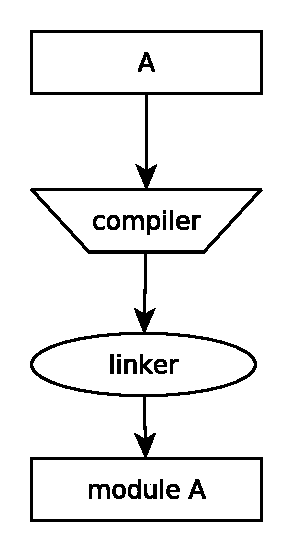
\includegraphics[width=0.20\linewidth]{figures/basic_module_compilation.pdf}
%   \caption{Construction du module A à partir des sources.}
% \end{figure}

%La création d'exécutable inclut deux étapes importantes, la compilation et
%l'édition des liens. La première étape consiste à prendre un fichier de code
%source et de le traduire en fichier objet, que l'on retrouve souvent avec
%l'extension \verb|.o| ou \verb|.obj|, qui contient la représentation des
%procédures compréhensible par le processeur. Ces fichiers objets ne sont pas
%encore exécutable pour autant, il faut tout d'abord effectuer la seconde étape,
%qui va les regrouper en un exécutable. Le programme qui s'occupe de l'édition
%des liens est le \textit{linker}, la version GNU se nomme \verb|ld|.  Voici
%l'exemple de la création d'un exécutable composé des fichiers sources C
%\verb|main.c| et \verb|foo.c|:
%
%\begin{figure}[ht]
%    \begin{minipage}[t]{0.5\textwidth}
%\begin{verbatim}
%# Compilation
%gcc -c main.c -o main.o
%gcc -c foo.c -o foo.o
%# Édition de liens
%ld -o main.exe main.o foo.o
%\end{verbatim}
%    \end{minipage}
%
%    \caption{Exemple de création d'un exécutable}
%\end{figure}



%Cela implique que ils possible de retrouvé une dépendance en diamant tel que représenter
%dans la figure-\ref{fig:dep1} qui peut causer un problème. % Détailler
%\begin{figure}[ht] %% Pas juste valide pour scheme.
%  \begin{center}
%    %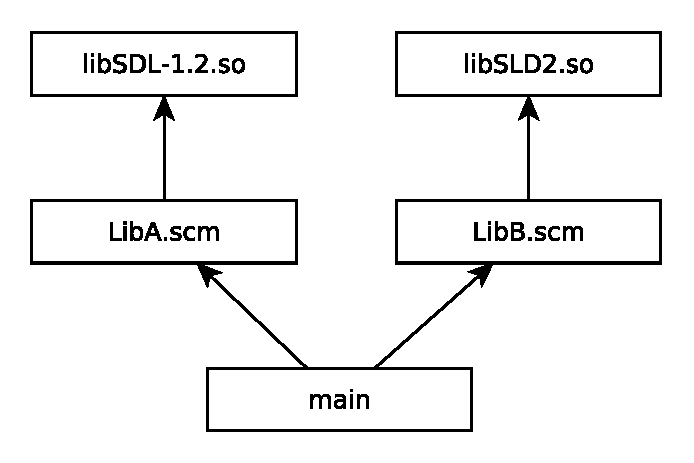
\includegraphics[width=4cm]{figures/SchemeLibrary}
%    \caption{Dépendence en diamant}
%    \label{fig:dep1}
%  \end{center}
%\end{figure}

%% NOTE: Soit P un processus, execution(A, P=[A,B]) == execution(A, P=[A]).
%Soit un processus \textbf{P} qui réfère aux bibliothèques \textbf{A} et \textbf{B}.
%Une bibliothèque peut masquer les symboles d'une autre bibliothèque chargé dans le même processus.
%La bibliothèque \textbf{A} coexiste avec la bibliothèque \textbf{B} si la \textbf{A}
%ne masque pas des symboles ne \textbf{B} qui amène un comportement non défini.


% Historiquement, il y avait un problème avec la coexistence entre deux dll sous Window. TODO: devellopper

% - Système distribué (Actor), non limité par la diversité des bibliothèque.


% TODO:
%La coexistance entre plusieurs versions d'une même bibliothèque
%===========================================================
%
% - Définition d'une bibliothèque
%   - Nom symboles:
%     - Fonction
%     - Variables global
%     - Structure de donnée
%     - Macro (Compilation)
%
%- Définition par coexistence de plusieurs bibliothèque.
%- Pourquoi est-ce utile?
%- Conditions nécessaire pour la coexistence entre plusieurs versions d'une même bibliothèque soit possible.
%  - Data race.
%  - État partagé.
%- Système d'exploitation (DOS)




\chapter{Bibliothèque Scheme}
%% Bonne place???
Le langage Scheme\cite{Scheme} supporte plusieurs paradigme de programmation
comme la programmation fonctionnel, impérative et méta. Il a été conçu en 1975
par Guy L. Steele et Gerald Jay Sussman. C'est un langage de programmation à
avec typage dynamique basé sur les \textit{s-expression}s, qui consiste en des listes
parenthésés. Contrairement aux langages comme Javascript, C/C++ qui utilisent une
forme infixe pour les expressions, Scheme utilise une forme préfixé. Cela
signifie que l'opération est le premier élément de la listes suivie des
arguments. Un programme Scheme est donc une séquence de listes préfixés.  Chaque
\textit{s-expression} correspond soit à une application de procédure ou à une
application de macro.

\begin{table}[htbp]
\begin{center}
\begin{tabular}{|l|l|}
  \hline
  \textbf{Préfixe}& \textbf{Infixe}\\\hline
  \begin{mplisting}{0.1}
(+ 1 2)
\end{mplisting}&
  \begin{mplisting}{0.1}
1 + 2;
\end{mplisting}\\
\hline
  \begin{mplisting}{0.25}
(proc a1 a2 a3)
\end{mplisting}&
  \begin{mplisting}{0.25}
proc(a1, a2, a3);
\end{mplisting}\\
\hline
%    \begin{mplisting}{0.25}
%(if e1
%    e2
%    e3)
%\end{mplisting}&
%    \begin{mplisting}{0.25}
%if(e1)
%  e2;
%else
%  e3;
%\end{mplisting}\\
%\hline
\end{tabular}
\end{center}
  \caption{Comparaison entre syntaxe préfixe et infixe.}
\end{table}

La définition des associations globales est effectuée avec \lstcode{define}.  Cette
forme spécial associe un nom avec une valeur qui a un type quelconque.  Les types de
donnée disponible en Scheme sont \lstcode{boolean}, \lstcode{pair},
\lstcode{symbol}, \lstcode{number}, \lstcode{char}, \lstcode{string},
\lstcode{vector}, \lstcode{port} et \lstcode{procedure}.

Les procédures sont des objets de premier classe, cela signifie qu'ils peuvent
être manipulé comme les autres types de donnée. Ils peuvent
être passés en paramètre d'un procédure et retournés comme résultat.
Certaines fonctions -- tel que \lstcode{map}, \lstcode{fold}, etc. -- bénéficie
que les procédures sont des objets de premier classe.

\section{Fonction et Procédure}

Les procédures et les fonctions sont définit par le constructeur
\lstcode{lambda}.  La syntaxe pour un lambda est \lstcode{(lambda args
body...)}.  Les éléments \lstcode{args} et \lstcode{body...} correspondent
respectivement à la liste d'arguments et au corps de la procédure, qui est
composé d'au moins une \textit{s-expression}. Le mode de passage de paramètre
utilisé lors de l'application d'une procédure est par valeur.  Cela signifie
que chaque argument est évalué avant d'être passé à la procédure.

% \begin{figure}[ht]
%   \begin{center}
%     \begin{tabular}{|l|}
%       \hline
%     \begin{mplisting}{0.55}
% (define fact
%   (lambda (n) (if (= n 0) 1
%                   (* n (fact (- n 1))))))
% \end{mplisting}\\\hline
%     \end{tabular}
%   \end{center}
%   \label{fig:fact1}
%   \caption{Voici une implémentation de la fonction factoriel en Scheme.
%   Cela montre un exemple de récursion.}
% \end{figure}

% READ Distinguer macro procedure.
\begin{figure}[ht]
  \begin{center}
    \begin{tabular}{|l|}
      \hline
    \begin{mplisting}{0.8}
(define map
  (lambda (f lst) (if (pair? lst)
                      (cons (f (car lst)) (map f (cdr lst)))
                      lst)))
\end{mplisting}\\\hline
    \end{tabular}
  \end{center}
  \label{fig:fact1}
  \caption{Voici une implémentation de la fonction d'ordre supérieur \lstcode{map} en Scheme.
  Cela montre un exemple utilise les procédure comme des objets de première classe et
  aussi un exemple d'application récursive.}
\end{figure}


\section{Les Macros}
\label{sec:ch2_macro}

Les listes sont une structure principale du langage,
Scheme peut facilement manipuler les liste, donc Scheme peut manipuler du code.

%% XXX: suite 1.

Le langage Scheme offre des constructions qui permettent la transformation
du code source. Ce sont les macros, certain langage comme C et C++ offre un système
de préprocesseur qui ce limite à une simple substitution textuelle. Les macros en Scheme
sont des procédure Scheme avec toute les capacités de calcule.

Les macros sont une forme de procédure qui manipule la structure du code
plutôt que des valeurs. Il sont définit soit par la forme \lstcode{define-macro}
où \lstcode{define-syntax}.
\begin{figure}[ht]
  \begin{tabular}{|l|}\hline
\begin{mplisting}{0.65}
(define-macro (include filename)
  (with-input-from-file
    filename
    (lambda ()
      (cons 'begin
        (read-all (current-input-port) read)))))
\end{mplisting}\\\hline
\end{tabular}
\end{figure}

%% XXX: suite 2.
La structure des bibliothèque définit dans le depuis le standard
R4RS\cite{Scheme:R4RS} et R5RS\cite{Scheme:R5RS} consistait simplement de
fichiers Scheme qui sont importés dans le module courant. Cette importation est
effectué soit par la procédure \texttt{load} ou par la forme spéciale
\texttt{include}. Ce modèle de bibliothèque possède plusieurs lacunes.

%% Gambit doc
\begin{itemize}
  \item Ce modèle de chargement n'est pas à l'abri des chargements multiples
    d'un module qui amène soit la duplication de code ou la réévaluation
    non désiré d'un code.

  \item Toutes les déclarations dans un module sont ajoutés à l'environnement
    global lors de l'importation. Cela amène des conflits de nom entre les
    symboles du module principale et les modules importés.

  \item L'importation d'un module par \texttt{load} nécessite le chemin exacte
    du module à importer qui peut être soit relatif ou absolu.  Un chemin
    relatif prend comme origine le répertoire présent.  L'importation d'un
    module par \texttt{include}, contrairement au \texttt{load}, le chemin
    relatif prend comme origine l'emplacement du fichier dans lequel la forme
    spécial \texttt{include} ce situe.

\end{itemize}


Lors d'un chargement de bibliothèque par \texttt{load} les macros sont expansé
et le code résultant est exécuté. Pour avoir accès aux macros, il faut utiliser la
forme spécial \texttt{include} qui est expansé par le contenu du fichier.
L'expression \lstcode{(include "foo#.scm")} est remplacé par le contenu du fichier
\lstcode{foo#.scm}. L'inclusion tout comme un \lstcode{load} nécessite le chemin
absolu ou relatif du fichier. L'exemple \ref{fig:r4rs_fact} montre un exemple
de module simple n'utilisant que \lstcode{load}.

\begin{figure}[ht]
  \begin{center}
    \begin{tabular}{|l|}
    \hline
    \begin{mplisting}{0.4}
;; fact.scm
(define (fact n)
  (if (< n 2)
    n
    (* n (fact (- n 1)))))
\end{mplisting} \\\hline
    \begin{mplisting}{0.4}
;; main.scm
(load "fact.scm")
(display (fact 5))
\end{mplisting} \\\hline
    \end{tabular}
  \end{center}
  \caption{Le fichier \texttt{fact.scm} est un exemple de module R4RS exposant
  la fonction mathématique \lstcode{fact}. Le fichier \texttt{main.scm} est un
  programme principal qui utilise le module \texttt{fact.scm}.}
  \label{fig:r4rs_fact}
\end{figure}

Le modèle de bibliothèque utilisé dans les standard Scheme prior au
R6RS\cite{Scheme:R6RS} a comme désavantage qu'une bibliothèque peut masquer les
fonctionnalités d'une autre bibliothèque puisque le chargement effectué par la
procédure \texttt{load} est dans le contexte global. Bref, les procédures de la
bibliothèque \textbf{A} peuvent rentrer en conflit de nom avec les procédures
de la bibliothèque \textbf{B} s'ils sont chargé dans le même contexte.  Pour
évité ces conflit, il faut que chaque nom utilisé au sein des bibliothèques
soit distinct, ce qui rajoute une tâche au programmeur.

\todo{Citation to gambit}

Gambit offre un mécanisme pour aider a minimiser les conflits de nom. Ce
méchanisme permet d'associer un identifiant à un autre avec la forme spécial
\lstcode{##namespace}.  L'appel à \lstcode{(##namespace ("foo#" A B))} indique
qu'une référence succécante à \lstcode{A} devient une référence à
\lstcode{foo#A} et l'un à \lstcode{B} devient une à \lstcode{foo#B}. Le espace
de nom dans lequel \lstcode{A} et \lstcode{B} est \lstcode{foo#}.

\begin{center}
  \begin{figure}[h]
  \begin{tabular}{|l|}
\hline
\begin{mplisting}{0.5}
;; math#.scm
(##namespace ("math#" fact fib))
\end{mplisting} \\\hline
\begin{mplisting}{0.6}
;; math.scm
(##namespace ("math#" fact fib))
(define (fib n)
  (if (< n 2)
    n
    (+ (fib (- n 1)) (fib (- n 2)))))
(define (fact n)
  (if (< n 2)
    1
    (* n (fact (- n 1)))))
\end{mplisting}\\\hline
  \end{tabular}
  \caption{Écriture d'un petit module mathématique qui implémente les fonctions \lstcode{fact}
    et \lstcode{fib}. Ce module est séparé en 2 fichiers, \texttt{math\#.scm} est un fichier
    contenant les déclarations de l'espace de noms et des définitions de macros que le module
    exporte.}
  \label{fig:math_module1}
\end{figure}
\end{center}


Le concept de bibliothèque a été raffiné  dans le R6RS.  Le R6RS rend le
support de la procédure \texttt{load} optionnel et ajoute une forme spéciale
\texttt{library} pour définir des bibliothèques et une autre forme spéciale
\texttt{import} pour gérer la inclure une bibliothèque.  Les noms utilise
pour nommer une bibliothèque peuvent seulement contenir des symboles et des
numéros de versions à la fin. Les expression import et export doivent seulement
apparaître une seul fois dans le définition de la bibliothèques.

Les bibliothèques ainsi définit, lie chaque procédure à la bibliothèque.  Cela
permet la réutilisation des mêmes identificateurs dans deux bibliothèque
différente.  Les conflits de nom sont gérés lors de l'importation des la
bibliothèques. L'importation d'un module est permit au sein d'une bibliothèque
comme dans un programme principale. La syntaxe d'un import reste identique dans
ces deux cas.


%\begin{center}
%  \begin{figure}[h]
%  \begin{tabular}{|l|l|}
%\hline
%\begin{mplisting}{0.5}
%;; Library
%(library (math)
%  (export fact)
%  (import (rnrs base))
%  (define (fact n)
%    (if (< n 2)
%      1
%      (* n (fact (- n 1))))))
%\end{mplisting} &
%\begin{mplisting}{0.5}
%;; Main program
%(import
%  (rnrs base)
%  (rnrs io simple)
%  (math))
%
%(display (fact 5))
%(newline)
%\end{mplisting}\\\hline
%  \end{tabular}
%\caption{À gauche, il y a un exemple d'une bibliothèque mathématique dans le format R6RS qui implémente
%la fonction factoriel. À droite, un exemple d'importation de la bibliothèques qui utilise la forme
%spéciale \texttt{import}.}
%\end{figure}
%\end{center}

L'implémentation des bibliothèques Scheme est basé sur le standard R7RS qui
conserve la procédure \texttt{load} que le R6RS enlève et remplace la structure
des bibliothèques.  Une bibliothèque en R7RS utilise la forme spécial
\texttt{define-library} au lieu de \texttt{library}. Ces deux formes ont
beaucoup de similarité, il n'est pas difficile de passé d'une bibliothèque R6RS
à une bibliothèque R7RS. Takashi Kato a publié un article au \emph{Scheme
Workshop} 2014 qui explique une procédure pour transformer un module R6RS en
R7RS \cite{SW2014:R6RS/to/R7RS}.  L'extension de fichier utilisé par les
définitions des bibliothèques est \verb|.sld| qui signifie \emph{Scheme Library
Definition}.

\begin{center}
  \begin{figure}[h]
  \begin{tabular}{|l|l|}
    \hline
    \begin{mplisting}{0.5}
;; Library R6RS
(library (math)
  (export fact)
  (import (rnrs base))
  (define (fact n)
    (if (< n 2)
      1
      (* n (fact (- n 1))))))
\end{mplisting} &
    \begin{mplisting}{0.5}
;; Library R7RS
(define-library (math)
  (export fact)
  (import (scheme base))
  (begin
    (define (fact n)
      (if (< n 2)
        1
        (* n (fact (- n 1)))))))
\end{mplisting}\\\hline
  \end{tabular}
\caption{À gauche, il y a un exemple d'une bibliothèque mathématique dans le format R6RS qui implémente
la fonction factoriel. À droite, une réécriture de la bibliothèque de gauche en R7RS.}
  \label{fig:r6rs_r7rs_math_mdoule}
\end{figure}
\end{center}

La syntaxe \lstinline{import} définit dans le R7RS indique le nom de
de la bibliothèque à collecter en plus des information sur les composante
à importer.
\begin{figure}[ht]
  \begin{mplisting}{0.9}
(import (only (gambit thread) make-thread thread-start! thread-join!))
\end{mplisting}
  \caption{Importation d'un sous-ensemble des fonctionnalité de la bibliothèque}
\end{figure}

% - (import (foo)) ; exportant f1 f2 f3
% ===>
% - (##demand-module foo)
% - (##namespace ("foo") f1 f2 f3)
% - macros
% - (##namespace (""))

\section{Chargement des bibliothèques}


Un système est composé d'un ensemble d'éléments (modules) qui interagissent
entre eux.  Une bibliothèque fait office de module au sein d'un système simple
ou complexe.
%La collection des modules s'effectue au sein d'un

% TODO: voir chargé
Le chargement d'une bibliothèque Scheme (ou module) est séparé en plusieurs niveaux.
% TODO: now
Les bibliothèques sont soit lu du disque vers la mémoire durant l'exécution
ou déjà dans la mémoire du processus. Durant la compilation les modules sont
collecté pour construire un exécutable. Le chargement
d'une bibliothèque inclut une phase de recherche sur le système de fichier pour valider
l'existence de la bibliothèque et des fonctionnalités demandés. L'emplacement des
bibliothèques sur le système de fichier est lié par défaut aux chemin spécifié par
le \lstinline{##module-search-order} a comme défaut \lstinline{~~lib} et \lstinline{~~userlib}.


La procédure exacte de chargement des bibliothèques par \verb|import|
n'est pas spécifier par le standard R7RS. Le standard spécifie seulement la syntaxe
à utilisé et le de comportement principal qui est
requis. L'importation d'une bibliothèque doit chargé la bibliothèque
et rendre c'est fonctionnalité disponible dans le contexte
l'importation a eu lieu qui peut soit ovenir d'un programme principale
ou d'une bibliothèque.

Le chargement d'une bibliothèque peut-être effectuée à l'exécution par
l'utilisation de \texttt{eval} (par \texttt{load}) pour les fichiers source et
\texttt{load-objcet-file} pour les bibliothèques compilées. Cette recherche
peut aussi avoir lieu durant l'édition des lien en utilisant les méta-infos
contenus dans les \textbf{.c} qui sont chacun compilé par le compilateur C
en \textbf{.o} et lié par le \textit{linker}.

\section{Modèle dynamique}
Dans ce modèle les bibliothèques sont lié au programme durant l'exécution. Cela
nécessite que les bibliothèques soit organisé sur le système de fichier d'une façon
distingable. Chaque module doit posséder un nom unique qui permet d'y référer.
Ce nom unique va être utilisé lors de la collection des dépendances.


%Les bibliothèques
%sont soit en code source ou compilé nativement avec l'extension (\textit{.oN})
%où le N correspond à la version du binaire qui commence à 1.


La recherche des bibliothèques est éffectué dans un ordre spécifique
indépendant de la spécification.  L'algorithme de recherche les bibliothèques
prend entré le nom de la bibliothèque et retourne le chemin absolu
correspondant à sont emplacement dans l'arborescence du système de fichier. Les
bibliothèques sont situées dans différents répertoires l'origine du programme,
le répertoire des bibliothèques système (\lstinline{~~lib}) et le
répertoire de bibliothèque utilisateur (\lstinline{~~userlib}).

% \begin{itemize}
%   %% XXX: directory where the executable is located (usefull for devel no need to install the module). collecté
%   \item \verb|origin/dummy.sld|
%   \item \verb|origin/dummy/dummy.sld|
%   \item \verb|~~userlib/dummy.sld|
%   \item \verb|~~userlib/dummy/dummy.sld|
%   \item \verb|~~lib/dummy.sld|
%   \item \verb|~~lib/dummy/dummy.sld|
% \end{itemize}

Chaque module possède trois niveau d'initialisation dans le système numéroté de
0 à 2. Le niveau 0 indique que le module n'a pas été initialisé. Ces les niveau
des module qui ont juste été collecté par le système. Le niveau 1 indique que
le descripteur du module à été récupéré. L'étape 2 est utilisé pour indiquer
les module chargé.

Soit un système avec les dépendance suivante:
\begin{figure}[ht]
  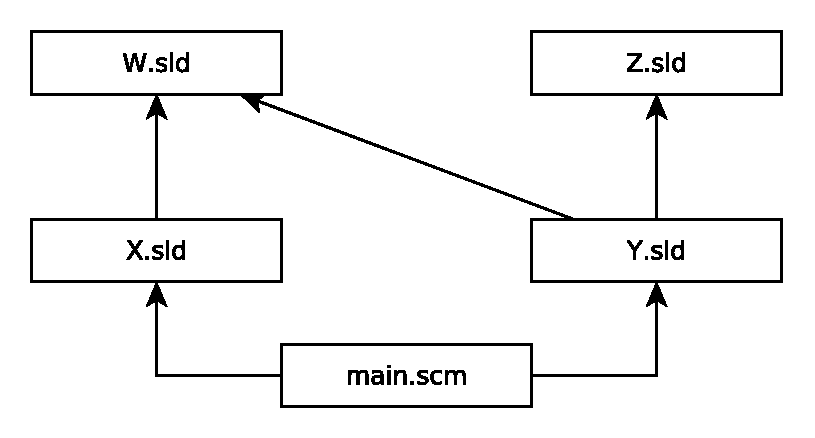
\includegraphics{figures/system-example}
  \caption{Un exemple d'un système fictif composé de différents modules.
  Le module principale se nomme utilise l'extension \textbf{.scm}
  et les bibliothèques porte l'extension \textbf{.sld}}
\end{figure} % TODO: use yed for that graph


Le démarrage du module principal Main.scm déclenche la collection des modules X
et Y, qui récursivement déclenche la collection de W et Z. L'algorithme de
collection des modules ignore les module qui apparaisse plusieurs fois au sein
du graphe.

Une fois la collection de tous ces modules est complété le descripteur de
module est récupéré par un appels à \verb|dlopen| et \verb|dlsym| dans le cas
compilé.


\section{Module hébergé}

Un module qui est hébergé est un module qui dont son contenu
se retrouve sur un domain comme \url{github.com}.


\begin{figure}[ht]
\begin{lstlisting}
hostname      = +( domainlabel "." ) toplabel
domainlabel   = alphanum | alphanum *( alphanum | "-" ) alphanum
toplabel      = alpha | alpha *( alphanum | "-" ) alphanum
alphanum      = alpha | digit
alpha         = [a-zA-Z]
digit         = [0-9]
\end{lstlisting}
  \caption{Grammaire BNF représentant un hostname selon un sous
  ensemble du RFC-2396.}
\end{figure}

La différence avec la spécification du hostname dans le RFC-2396
est que le hostname ne peut pas finir par un point et doit contenir
au moins un \verb|domainlabel|. C'est pour permettre de distingué
un module local et un module hébergé.

\subsection{Module gambit/git}

Ce module offre un interface pour utiliser interagir avec les des dépôts git.
Il permet de cloner un dépôts qui est hébergé sur \url{github.com}. Un clone du
dépôts est simplement un copie qui contient les informations suffisantes pour
passer d'une version d'un module à un autre. L'opération qui permet de changer
de version est \emph{checkout}.


%-------------------------------------------------------------------------------
%
%Modèle "link dynamique" :
%  recherche des libs au run time, utilisation de eval (par load) et
%  load-object-file
%
%  % gsi main.scm      ou      % gsc main.scm ; gsi main.o1
%
%    origin/main.scm    : (import X Y)
%          /X/X.sld     : (import)
%
% ~~userlib/Y/Y.sld     : (import Z)
%
%     ~~lib/Z/Z.sld     : (import)
%          /Z.o1
%
%-------------------------------------------------------------------------------
%
%Modèle "link statique" :
%  recherche des libs au link time en utilisant les méta-infos
%  dans les .c (demand-lib et supply-lib), chaque .c compilé en
%  un .o séparément et les .o linkés par le compilateur C
%
%  % gsc -obj -keep-c X.sld      ;; créer .c et .o
%  % gsc -obj -keep-c Y.sld      ;; créer .c et .o
%  % gsc -obj -keep-c Z.sld      ;; créer .c et .o
%  % gsc -obj -keep-c main.scm   ;; créer .c et .o
%  % gsc -exe main.c             ;; combine les .o pour créer main.exe
%
%    origin/main.scm    : (import X Y)
%          /main.c      : (demand-lib X Y)
%          /main.o
%          /X/X.sld     : (import)
%            /X.c       : (demand-lib) (supply-lib X)
%            /X.o
%
% ~~userlib/Y/Y.sld     : (import Z)
%          /Y/Y.c       : (demand-lib Z) (supply-lib Y)
%          /Y/Y.o
%
%     ~~lib/Z/Z.sld     : (import)
%          /Z/Z.c       : (demand-lib) (supply-lib Z)
%          /Z/Z.o
%
%-------------------------------------------------------------------------------
%
%Modèle "whole-program" :
%  recherche des libs au compile time en utilisant les imports
%  dans les fichiers sources, les AST de toutes les libs fusionnées
%  en un seul AST compilé par gsc (donc un seul .c généré et compilé
%  par le compilateur C pour créer main.exe)
%
%  % gsc -exe -whole-program main.scm
%
%    origin/main.scm    : (import X Y)
%          /X/X.sld     : (import)
%
% ~~userlib/Y/Y.sld     : (import Z)
%
%     ~~lib/Z/Z.sld     : (import)
%
%-------------------------------------------------------------------------------
% correction d’une petite coquille…
% /Y.c       : (demand-lib Z) (supply-lib Y)
% /Y.o
%
% ~~lib/Z/Z.sld     : (import)
% /Z.c       : (demand-lib) (supply-lib Z)
% ...


% (check-sld "/tmp/scheme/base/base.sld" "/tmp/scheme/base")
% (check-sld "/tmp/scheme/base.sld" "/tmp/scheme")
% (check-sld
%  "/home/frederic/Documents/MasterResearch/gambit9/lib/cocolappin/scheme/base/base.sld"
%  "/home/frederic/Documents/MasterResearch/gambit9/lib/cocolappin/scheme/base")
% (check-sld
%  "/home/frederic/Documents/MasterResearch/gambit9/lib/cocolappin/scheme/base.sld"
%  "/home/frederic/Documents/MasterResearch/gambit9/lib/cocolappin/scheme")
% (check-sld
%  "/home/frederic/Documents/MasterResearch/g9/lib/scheme/base/base.sld"
%  "/home/frederic/Documents/MasterResearch/g9/lib/scheme/base")
% object-file-path: /home/frederic/Documents/MasterResearch/g9/lib/scheme/base/.gambit_409003@C/base.o1
% ("/home/frederic/Documents/MasterResearch/g9/lib/scheme/base/base.sld"
%  .
%  #<input-port #2 "/home/frederic/Documents/MasterResearch/g9/lib/scheme/base/base.sld">)

\chapter{Modules systèmes}
\label{ch:module_systems}





% Définition sommaire d'une bibliothèque de code
Une bibliothèque de code est le regroupement de plusieurs types de données, des
entiers, des nombres à virgule flottant, des chaînes de caractères, des
fonctions et des données composites. L'ensemble de ces données constitue les
fonctionnalités de la bibliothèque.  Les fonctionnalités d'une bibliothèque
peut être copié dans l'exécutable (bibliothèque statique), cela facilité la
distribution du binaire puisque que ses dépendances sont inclus dans
l'exécutable.  Les fonctionnalités d'une bibliothèque peuvent aussi être chargé
à l'exécution (bibliothèque partagés), cela permet de partagé des routine
commune entre plusieurs processus (programme en exécution). Les données de la
bibliothèque, par contre, ne sont partagé, chaque processus réfère à sa propre
version des données.  Le format d'une bibliothèque de code varie d'un langage à
l'autre et aussi d'un système d'exploitation à un autre. Les langages
interprétés utilisent plus souvent le code source directement ou une
représentation intermédiaire comme format pour les bibliothèques de code.  Pour
les langages compilés, c'est le format natif correspondant au système
d'exploitation qui est le plus souvent utilisé. Le système d'exploitation Linux
utilise le format ELF (\textit{Extensible Linking Format}), Microsoft Window
utilise le format PE (\textit{Portable Executable}) et MacOSX utilise le format
Mach-O (\textit{Mach object}) pour les exécutables et les bibliothèques.
% XXX: bytecodes aussi pour les langage compilé.

%Les langages
%de programmation interprétés fournisse leurs bibliothèques directement
%en code source. Dans cette catégorie, il y a Ruby, Python, Perl, Lua et
%Scheme -- dont le code des bibliothèques est écrit et frounit dans le
%langage respectif. Les langages compilés -- comme C, C++, C\# et Java --
%utilisent plutôt des formats binaires destiné, soit à une machine virtuelle
%(e.g. la \textit{Java Virtual Machine} JVM ou un architecture
%physique (e.g. i686, x86\_64, ARM). Les bibliothèques natives peuvent
%être utilisé


\section{Édition de liens dynamique}

Une application qui utilise une bibliothèque partagés ne contient pas le code
de la bibliothèque, mais plutôt le nom des fonctionnalités utilisés.  La
routine qui permet de récupérer la fonctionnalité à partir du nom est la
résolution qui est effectué par le \textit{dynamic loader}.  Lorsqu'un
programme lié dynamiquement à plusieurs bibliothèques partagés exécute du code
externe \verb|foo|, un routine de résolution est démarré pour déterminé quelle
bibliothèque lié au fournit la fonctionnalité \verb|foo|.

%% Bibiothèque dynamique native.
Par exemple, sous Linux l'utilitaire <<yes>>, qui est écrit en C,
est lié aux bibliothèques systèmes suivantes:
\begin{verbatim}
  linux-vdso.so.1 (0x00007ffeef7f9000)
  libc.so.6 => /usr/lib/libc.so.6 (0x00007ff68161c000)
  /lib64/ld-linux-x86-64.so.2 => ...
\end{verbatim}
La bibliothèque \textit{libc.so.6} contient la plupart des fonctions
standards du système sous Linux dont les fonctionnalités sont résolut
à l'exécution.
% Le but d'une bibliothèque est la réutilisation de code.
Dans le contexte d'un exécutable natif, le chargement des bibliothèques
s'effectue au début de l'application, avant l'exécution de la fonction principale
souvent nommé \textbf{main}. Plusieurs bibliothèques peuvent coexister simultanément au
sein d'un même processus sans que l'exécution du programme en soit affecté.

La résolution des fonctionnalité de ces bibliothèques sont effectué par un programme adapté
le \textit{program interpreter} du système qui correspond à \textit{/lib64/ld-linux-x86-64.so.2}.
Il est possible de forcer la résolution d'une fonctionnalité d'une bibliothèque
de façon manuel. Ce genre d'interaction est possible sur
les trois principales plateformes utilisées sur le marché (Windows, MacOSX et Linux).

%% TODO: continue here FIXME
Sur Linux, l'API qui permet d'interagir avec les bibliothèques partagés provient de \textit{libdl.so}.
Elle contient les fonctions \textit{dlopen}, \textit{dlsym}, \textit{dlerror} et \textit{dlclose} pour gérer
des bibliothèques de code supplémentaire chargé manuellement à l'exécution.  Pour charger la fonction
\textit{foo}, qui ne prend pas d'argument et ne retourne rien de la bibliothèque \textit{libFoo.so} en C,
il faut exécuter les deux appels suivant:
\begin{center}
  \begin{figure}[ht]
\begin{lstlisting}[language=C,frame=single]
  ...
  void *handle = dlopen("./libFoo.so", RTLD_LAZY);
  void (*foo)() = dlsym(handle, "foo");
  ...
\end{lstlisting}
\caption{Chargement dynamique de la bibliothèque \textit{libFoo.so} et
résolution de la fonction \textit{foo} sans gestion d'erreur sous Linux}
  \end{figure}
\end{center}
L'équivalent des bibliothèques partagés sous Window sont les DLLs, ils peuvent être chargé de façon similaire dans un
programme en utilisant les fonctions \textit{LoadLibrary}, \textit{LoadLibraryEx} et \textit{GetProcAddress}. Ils
fonctionne de la même façon que leur équivalent Linux. Pour MacOSX, il faut passer par les routines:
\begin{itemize}
    \item \textit{NSCreateObjectFileImageFromFile}
    \item \textit{NSLinkModule}
    \item \textit{NSLookupSymbolInModule}
    \item \textit{NSAddressOfSymbol}
\end{itemize}

La majorité des langages interprétés permettent l'importation de bibliothèque de code natif, via un interface
nommé \textit{foreign function interface}.
Prenons comme exemple les langage Python, Ruby, Lua et Scheme. Python possède le module ctypes
qui permet de chargé des bibliothèques natives dynamique, Ruby possède le module ffi.
%Ces modules ne font qu'encapsuler les fonction de chargement de bibliotheques native pour qu'il puisse être invoqué
%dans le langage cible.

% Bibliothèque Lua en C
% - La bibliothèque doit avoir le même nom que celui utilisé par le \textit{import}.

Certains langages ont même un mécanisme pour charger des bibliothèques natives s'ils ont été conçus spécialement.
Dans le langage de programmation Lua, il est possible en Lua de chargé directement
une bibliothèque dynamique si elle contient une fonction principale \textbf{luaopen\_\textit{libname}}
où \textit{libname} est le nom de la bibliothèque.

Gambit Scheme utilise un mécanisme équivalent. Il permet le chargement de ces modules qui ont été compilé
en bibliothèque partagé (DLL) avec la fonction \textit{(\textbf{load} "libname")}. Le chargements de la
bibliothèque ressemble à celui de Lua.

%% Python
%\begin{figure}[ht]
%\begin{lstlisting}[language=python,frame=single]
%# From https://docs.python.org/2/library/ctypes.html
%from ctypes import *
%# Chargement d'une bibliotheque native.
%lib = cdll.LoadLibrary("./libFoo.so")
%# Appel de la fonction foo.
%lib.foo()
%\end{lstlisting}
%\caption{Code d'importation de la fonction \textbf{foo} de la bibliothèque \textit{libFoo.so} en Python}
%\end{figure}

\begin{center}
% Ruby
\begin{figure}[ht]
\begin{lstlisting}[language=ruby,frame=single]
require 'ffi'
# Chargement d'une bibliotheque native.
module LibFoo
    extend FFI::Library
    ffi_lib './libFoo.so'
    attach_function :foo, [], :void
end
# Appel de la fonction foo.
LibFoo.foo
\end{lstlisting}
\caption{Code d'importation de la fonction \textbf{foo} de la bibliothèque \textit{libFoo.so} en Ruby}
\end{figure}
\end{center}

La résolution des fonctionnalités effectué par le \textit{dynamic linker} utilise un ordre de recherche
définit. Cet ordre de recherche inclut l'exécutable courant, les dépendances de l'exécutable, la bibliothèque
passé à \textit{dlsym}. La résolution d'une fonctionnalité par \textit{dlsym} qui n'engendre pas la résolution
d'un autre fonctionnalité externe n'utilise pas le programme principale dans l'ordre de recherche qui alors
commence par la bibliothèque passé à \verb|dlsym| suivit de ses dépendances. Les résolution de fonctionnalité
provenant d'appels indirecte au \textit{dynamic linker} inclut le programme principal et ses dépendances avant
la bibliothèque passé à \verb|dlsym|.

\begin{center}
    \begin{figure}[ht]
        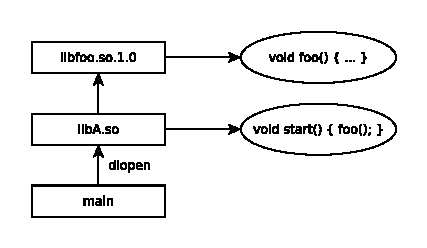
\includegraphics{figures/libdeps-ex1.pdf}
        \caption{Un exemple de dépendance de bibliothèques au sein d'un application simple fictive.
            La bibliothèque \textit{libA.so} est chargé dans l'application \texttt{main} via
            les appels au procédure \textit{dlopen} et \textit{dlsym}. Le fonctionnalités utilisés
            dans l'exemple sont marqué par un ellipse.
        }
        \label{fig:deps-ex1}
    \end{figure}
\end{center}

Dans la situation situation présenté dans la figure-\ref{fig:deps-ex1}, quels sont les étapes inclut
dans l'exécution de ce programme qui ne fait qu'appeler la fonctionnalité \texttt{start} de la
bibliothèque \textit{libA.so}. La fonctionnalité \texttt{start} est résolu de façon direct par
un appel à \verb|dlsym(libA, "start")|, qui commence la recherche de la procédure \texttt{start} dans
la bibliothèque spécifier dans \texttt{dlsym}. Le programme, une fois la procédure trouvé, l'exécute.
L'appel à une procédure non résolue (e.g.\ la procédure \texttt{foo} invoqué dans \texttt{start})
déclenche une procédure automatique de résolution des fonctionnalités. Cette procédure de résolution
commence sa recherche à partir de l'exécutable, puis itère la liste des dépendances directe. Si la
fonctionnalité n'est pas encore trouvé, la recherche continuera à partir de la bibliothèque passé à
\texttt{dlsym}.

% Stub

% TODO: exemple de résolution direct
Connaissant l'ordre de recherche du \textit{dynamic linker}, il est facile de construire un application avec des bibliothèques
qui cause un masquage de fonctionnalité. Deux possibilité facilement exploitable, faire que l'exécutable main fournisse
directement la fonctionnalité à masquer, ou avoir une des dépendances de l'exécutable contenant cette fonctionnalité. La figure-\ref{fig:deps-ex2}
en est l'exemple qui utilise la seconde méthode. La première consisterait à transformer l'exécutable main est bibliothèque
exécutable qui ne pourrait pas être supporté sur certaine plateforme. Sous Linux, il est possible de créer une bibliothèque qui
exécutable en passant le paramètre \texttt{-rdynamic} à \textit{gcc} lors de la construction.

\begin{center}
    \begin{figure}[ht]
        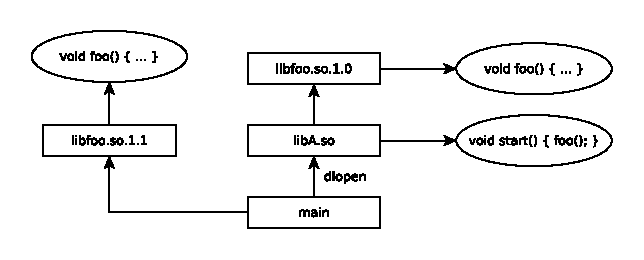
\includegraphics{figures/libdeps-ex2.pdf}
        \caption{Exemple de dépendance dans un application cause le masquage de la fonctionnalité \texttt{foo}
        de la bibliothèque \textit{libfoo.so.1.0} par la bibliothèque \textit{libfoo.so.1.1}}
        \label{fig:deps-ex2}
    \end{figure}
\end{center}
%% BEGIN
% D'autre langage compilé comme C/C++
% ne le permette pas directement, la liste des bibliothèques de code utilisé par un
% programme est déterminée lors de la création du fichier binaire, qui peut être
% soit un exécutable où une bibliothèque.
%% END


% TODO: pourquoi est-ce utile?
% XXX: structure pas final.
% - Les bibliothèques coexistent dans les application de tous les jours.
Analyser les interactions entre des bibliothèques au sein d'un même programme permet de
mieux comprendre quels sont les circonstance qui peuvent conduire à des comportements
non désirés, par exemple le masquage démontré dans la figure-\ref{fig:deps-ex2}.
Cela permet aussi d'établir les conditions qui inhibe ces comportements non désirés.



% TODO: shift chapter number.

\chapter{Implémentation des modules}
\label{ch:modules_implementation}

Ce chapitre traite de notre implémentation des modules dans Gambit qui se veut
le plus portable entre les différentes implémentations de Scheme.  Notre
approche des modules se base sur la syntaxe de R7RS.  Notre implémentation des
modules utilise des formes déjà existantes et aussi de nouvelles formes qui ont
été ajoutées au besoin.  Ces nouvelles formes nous ont permis d'intégrer la
syntaxe des modules R7RS avec les modules primitifs de Gambit. Il y a deux
façons d'écrire des modules.  Les modules primitifs sont utilisés pour
implémenter des fonctionnalités système dans Gambit, par exemple, un module qui
implémente une nouvelle syntaxe.  La syntaxe des modules R7RS est utilisée
lorsqu'un module se veut compatible avec d'autres implémentations du langage de
programmation Scheme supportant R7RS.


Les formats des modules R7RS, construits avec \lstcode{define-library}, contiennent
plusieurs composantes.
\begin{itemize}
  \item L'espace de nom du module qui regroupe toutes les fonctionnalités.
  \item Une liste des modules qui sont utilisés par le module courant.
  \item Une liste des symboles exportés par le module.
\end{itemize}
Il est possible de modifier les identifiants d'un module lors de l'importation et de l'exportation.
L'importation multiple d'un module doit correspondre à un seul chargement.
Pour exprimer les relations entre les modules certaines formes spéciales
ont été ajoutées dans Gambit.  Si les concepteurs de bibliothèques respectent
la syntaxe R7RS, alors il est possible de l'importer dans Gambit. C'est indépendant
du système Scheme pour lequel les bibliothèques ont été écrites.



% Le format des modules nécessite plusieurs composantes.
% Chaque module a son propre espace de nom
% disjoint des autres modules. Un liste d'importation
% qui indique les dépendances entre les modules et permet
% l'interaction entre les modules. Certaines formes spéciales
% ont été ajouté dans pour pouvoir exprimer les relation entre
% les modules. Les modules R7RS permette de spécifier les identifiant
% d'un module et de les renommer. Les relations entre les modules doivent
% pouvoir être exprimées.  La liste des modules requis par le module
% courant et les modules publiés par le module courant.

% - Créer un espace pour les modules.
% - Spécifier les dépendence. (2)
% - Spécifier les paramètre de compilation.
\section{La notation des fichiers dans Gambit}
%[TODO: notation ~~]
Gambit utilise une notation qui est compatible avec l'environnement du
système hôte. Il permet de référer au répertoire maison de l'utilisateur
et aux répertoires d'installation.

Un chemin est une chaine de caractère qui dénote une ressource.
Le séparateur des composantes d'un chemin dépend du système
d'exploitation, Linux et macOS utilise `/' alors que MSDOS et
Microsoft Windows utilise `$\backslash$`.

La notation qui permet de référer au répertoire maison de l'utilisateur
courant est par la notation `\url{~}' qui n'est pas suivit d'un `\url{~}'.
Le nom qui suit `\url{~}' est le nom de l'utilisateur. Par exemple,
\url{~USER} représente le répertoire de l'utilisateur {\tt USER}.

Un répertoire d'installation commence par les caractères `\url{~~}'. S'il n'y
a rien qui suit ces caractères alors c'est le répertoire d'installation central.
Sinon ce qui suit le `\url{~~}' est le nom du répertoire d'installation. Par
exemple, `\url{~~lib}' est le chemin vers le répertoire d'installation `\url{lib}'
des bibliothèques système de Gambit. Il est a noté que Gambit permet de redéfinir
l'emplacement des répertoires d'installation par l'utilisation de l'option d'exécution
`\verb|-:~~NAME=DIRECTORY|'.

\section{La forme \lstcode{\#\#namespace}}

Un identifiant est un symbole, utilisé dans le code, qui n'est pas sous un
\lstcode{quote}. Par exemple \lstcode{pair?} est l'identifiant de la procédure
qui teste que le type de donnée est une paire. Il est généralement lié à une
valeur ou une macro. Un symbole est un type de donnée primitif de Scheme.

Les espaces de nom sont gérés avec une forme spéciale propre à Gambit. Cette
forme se nomme \lstcode{##namespace} et permet de lier des identifiants à
d'autres identifiants dans le code. Cela affecte l'ensemble des identifiants
spécifiés dans la forme \lstcode{##namespace}, l'ensemble vide correspond à
tous les identifiants. Cette forme s'applique uniquement aux identifiants de
variable et de macro. Elle ne s'applique pas aux valeurs.  Cette forme
primitive est présente dans Gambit depuis longtemps.  Un espace de nom se
compose de n'importe quelle séquence de caractère terminé par un \lstcode{#}.
Il y a seulement l'espace de nom vide qui est une exception à cette règle et
c'est l'espace de nom par défaut.  Les associations de symboles données par la
forme \lstcode{##namespace} respectent la portée lexicale. Il y a trois types
d'opérations avec les espaces de nom.

Il y a les espaces de nom global qui s'applique à tous les symboles qui ne
contiennent pas de \lstcode{#}. \\
\begin{figure}[ht]
  \centering
  \lstset{language={scheme},frame=single}
  \begin{mplisting}{0.6}
(##namespace ("<ns>"))
;; <symbol-name> => <ns><symbol-name>
\end{mplisting}
  \caption{Namespace Global}
  \label{fig:forms->namespace-global}
\end{figure}

Il est possible de spécifier la liste des symboles qui sont affectés par la
déclaration d'espace de nom. À partir de la syntaxe de la figure
\ref{fig:forms->namespace-global}, il suffit d'ajouter les symboles après le nom
de l'espace de nom.\\
\begin{figure}[ht]
  \centering
  \lstset{language={scheme},
          frame=single}
  \begin{mplisting}{0.6}
(##namespace ("<ns>" A B ...))
;; A => <ns>A
;; B => <ns>B
;; ...
\end{mplisting}
  \caption{Namespace Set}
  \label{fig:forms->namespace-set}
\end{figure}

%Chaque symbole dans l'espace de nom peut être renommé à un nouveau symbole en
%spécifier une pair contenant l'association. La forme ressemble à l'exemple
La forme \lstcode{##namespace} permet aussi de lier un identifiant à un
autre identifiant dans un espace de nom donné. Chaque association est marquée
par une paire qui crée un alias entre le premier élément et le second. Par exemple,
la paire \lstcode{(<old> <new>)} remplace \lstcode{<old>} par \lstcode{<ns><new>}.\\
\begin{figure}[ht]
  \centering
  \lstset{language={scheme},
          frame=single}
  \begin{mplisting}{0.6}
(##namespace ("<ns>" (<old> <new>) ...))
;; <old> => <ns><new>
;; ...
\end{mplisting}
  \caption{Namespace Rename}
  \label{fig:forms->namespace-rename}
\end{figure}

% La syntaxe de la
% forme \lstcode{##namespace} qui inclus toutes les symboles dans l'espace de nom
% marqué par \lstcode{<ns>} est:

% \begin{center}
%   \begin{mplisting}{0.8}
% (##namespace ("<ns>"))
% \end{mplisting}
% \end{center}

% Il est possible de spécifier une liste des symboles qui appartiennent à
% l'espace de nom. Notez que seulement le espace de nom est entre guillemets.

% \begin{center}
%   \begin{mplisting}{0.8}
% (##namespace ("<ns>" sym1 ...))
% \end{mplisting}
% \end{center}


% L'utilisation de la forme \lstcode{##namespace} permet de associer plusieurs
% identifiant dans un espace de nom spécifique.  La procédure \lstcode{hello} est
% défini dans l'espace de nom \lstcode{hello#}.

Cette forme est utilisée pour créer un espace distinct pour chaque module.
Cela permet d'éviter les conflits de nom entre les identifiants des modules.
Chaque module commence par déclarer son espace de nom suivi des définitions
des procédures du module. Les différentes formes d'espace de noms sont données
par les figures \ref{fig:forms->namespace-global}, \ref{fig:forms->namespace-set}
et \ref{fig:forms->namespace-rename}.
\\
\begin{figure}[ht]
  \centering
  \lstset{language={scheme},
          frame=single}
\begin{mplisting}{0.6}
;; hello.scm
(##namespace ("hello#" hi))
(define (hi)
  (display "Hello, world!\n"))
(hi)
\end{mplisting}
  \caption{Module Hello}
  \label{fig:namespace->hello}
\end{figure}

L'exemple \ref{fig:namespace->hello} est un exemple d'utilisation de la forme
\lstcode{##namespace} pour créer un espace pour le module \lstcode{hello}.
La procédure \lstcode{hi} est dans l'espace de nom \lstcode{hello#}.

\section{La forme \lstcode{\#\#demand-module} et \lstcode{\#\#supply-module}}

Le mécanisme de chargement des modules est géré par la forme spéciale
\lstcode{##demand-module}. Cette forme indique au système de charger un module
s'il n'est pas déjà chargé. Cette forme gère le chargement multiple d'un
module. Elle est utilisée pour importer la liste des modules requis par le
module courant.  Le fonctionnement de cette forme est similaire à la procédure
\lstcode{load} avec quelques différences. La forme spécial
\lstcode{##demand-module} génère une expression vide. L'effet de cette
forme agit après la phase d'expansion des macros. Le paramètre passé à
\lstcode{##demand-module} doit être un symbole qui correspond au nom du module.
La procédure \lstcode{load} requiert le chemin complet vers le fichier à
charger.

Il est à noter que l'ordre dans lequel les \lstcode{##demand-module}
apparaissent correspond à l'ordre dont les modules sont visités. Cette forme
est permise partout où une définition de macro est permise.
%[TODO: ##demand-module]
%% Review.

% \begin{center}
%   \begin{mplisting}{0.9}
% (##demand-module A)
% (##demand-module A)
% (##demand-module B)
% \end{mplisting}
% \end{center}

Nous avons ajouté un forme spéciale conjointe au \lstcode{##demand-module}
pour indique le nom symbolique des modules des modules exportés. Cette
forme spéciale est \lstcode{##supply-module}, elle accepte comme paramètre le
nom du module exporté par l'entité courant.  La syntaxe de ces deux formes dans
la figure \ref{fig:syntax->demand/supply-module}.\\
\begin{figure}[ht]
  \centering
  \lstset{language={scheme},
          frame=single}
  \begin{mplisting}{0.8}
(##demand-module %*\textit{<module-ref>}*)
(##supply-module %*\textit{<module-ref>}*)
\end{mplisting}
  \caption{Syntaxe des formes \lstcode{demand-module} et \lstcode{supply-module}}
  \label{fig:syntax->demand/supply-module}
\end{figure}

\subsection{Les méta informations}
%
Il est utile d'attacher à un
module des informations qui sont accessibles lors de l'expansion
et même la compilation. Ces informations sont spécifiées par la forme
\lstcode{##meta-info}. Cette forme accepte au moins un paramètre qui
correspond au nom de la méta information, le reste des paramètres est la valeur
associée à la méta donnée.

\begin{center}
  \begin{mplisting}{0.5}
(##meta-info %*\textit{<name>}* %*\textit{<value>}*)
(##meta-info %*\textit{<name>}* %*\textit{<value>}* ...)
\end{mplisting}
\end{center}

Les méta informations sont utilisées pour donner des paramètres de compilation
du module. Les différentes méta informations sont \lstcode{cc-options},
\lstcode{ld-options}, \lstcode{ld-options-prelude}, \lstcode{pkg-config}
et \lstcode{pkg-config-path}. Ces méta informations ne sont utiles que pour les modules
compilés.

\begin{itemize}
  \item Les \lstcode{cc-options} sont ajoutés aux options de la commande qui
    invoque le compilateur C.

  \item Les méta informations \lstcode{ld-options} et \lstcode{ld-options-prelude}
    composent les paramètres de la commande qui invoque l'éditeur de lien.
    Les paramètres dans \lstcode{ld-options-prelude} précèdent ceux
    qui sont dans \lstcode{ld-options}.

  \item \lstcode{pkg-config} contient le nom des bibliothèques C à être
    liées au module Scheme. Les options nécessaires pour le compilateur
    C sont déterminées automatiquement par l'utilitaire \lstcode{pkg-config}.

  \item \lstcode{pkg-config-path} ajoute des répertoires à la variable d'environnement
    \lstcode{PKG_CONFIG_PATH} qui est utilisée par l'utilitaire \lstcode{pkg-config}.

\end{itemize}

\section{Implémentation des modules primitifs}

Un module primitif est généralement constitué d'un fichier d'entête avec la
déclaration de l'espace de nom et les définitions de macros et un fichier
contenant les procédures. Dans Gambit les fichiers d'entête sont marqués par un
\lstcode{#} juste avant l'extension, tel que \texttt{angle2/angle2\#.scm}.

\begin{itemize}
  \item \texttt{\textit{<name>}\#.scm} est la structure du nom fichier d'entête.
    Ce fichier contient des déclarations d'espace de nom et des
    définitions de macros.

  \item \texttt{\textit{<name>}.scm} est la structure du nom du fichier qui contient
    les procédures du module.

\end{itemize}

Le nom des fichiers doit correspondre à la dernière partie du nom de module.  Par
exemple, le module primitif \lstcode{angle2} doit inclure les fichiers
\lstcode{angle2/angle2.scm} et généralement \lstcode{angle2/angle2#.scm}.\\
\begin{figure}[ht]
  \lstset{language={scheme},frame=single}
\begin{mplisting}{0.9}
;; angle2/angle2#.scm
(##namespace ("angle2#" deg->rad rad->deg))
\end{mplisting}\\[4ex]
\begin{mplisting}{0.9}
;; angle2/angle2.scm
(include "angle2#.scm")
(##namespace ("angle2#" factor))
(##supply-module angle2)
(define factor (/ (atan 1) 45))
(define (deg->rad x) (* x factor))
(define (rad->deg x) (/ x factor))
\end{mplisting}
  \caption{Écriture d'un module qui implémente des fonctions de conversions
           entre les angles en degrés et en radian. Ce module est séparé en 2 fichiers.
           Le fichier \texttt{angle2/angle2\#.scm} contient les exportations et
           \texttt{angle2/angle2.scm} contient l'implémentation des
           fonctions.}
  \label{fig:module->angle}
\end{figure}

% XXX: END implementation
%\todo{Continuer ici}

%\begin{center}
%  \begin{figure}[h]
%  \begin{tabular}{|l|l|}
%\hline
%\begin{mplisting}{0.5}
%;; Library
%(library (math)
%  (export fact)
%  (import (rnrs base))
%  (define (fact n)
%    (if (< n 2)
%      1
%      (* n (fact (- n 1))))))
%\end{mplisting} &
%\begin{mplisting}{0.5}
%;; Main program
%(import
%  (rnrs base)
%  (rnrs io simple)
%  (math))
%
%(display (fact 5))
%(newline)
%\end{mplisting}\\\hline
%  \end{tabular}
%\caption{À gauche, il y a un exemple d'une bibliothèque mathématique dans le format R6RS qui implémente
%la fonction factoriel. À droite, un exemple d'importation de la bibliothèques qui utilise la forme
%spéciale \texttt{import}.}
%\end{figure}
%\end{center}

Dans l'exemple de la figure \ref{fig:module->angle}, il y a dans
\lstcode{angle2/angle2.scm} l'inclusion du fichier d'entête
\lstcode{angle2/angle2#.scm} qui ajoute une déclaration redondante de l'espace
de nom dans ce cas.  La déclaration \lstcode{(##namespace ("angle2#"))}
implique l'espace de nom ajouté par l'inclusion du fichier d'entête. Il est
possible que l'espace de nom déclaré dans \lstcode{angle2/angle2#.scm} soit
différent de celui utilisé dans \lstcode{angle2/angle2.scm}.

La forme \lstcode{##namespace} dans l'exemple \ref{fig:module->angle}
s'applique aux identifiants suivants:
\begin{center}
  \lstset{language={scheme},keepspaces=true}
  \begin{mplisting}{0.3}
factor    --> angle2#factor
deg->rad  --> angle2#deg->rad
rad->deg  --> angle2#rad->deg
\end{mplisting}
\end{center}

\subsection{La forme \lstcode{\#\#import}}
%
L'importation des modules est effectuée par la forme \lstcode{##import} qui
effectue deux actions, l'inclusion du fichier \lstcode{<name>#.scm} et un
chargement des définitions.  La forme \lstcode{##import}, comme
\lstcode{##demand-module} s'occupe de trouver l'emplacement du fichier d'entête
à partir du nom du module. Elle génère le \lstcode{##include} du fichier
d'entête s'il existe et un \lstcode{##demand-module} du module.  L'importation
\lstcode{(##import angle2)} est équivalente à:\\
\begin{figure}[ht]
  \centering
  \lstset{language={Scheme},frame=single}
  \begin{mplisting}{0.9}
(##include "/un/chemin/angle2/angle2#.scm")
(##demand-module angle2)
\end{mplisting}
  \caption{Expansion de \lstcode{(\#\#import angle2)}}
  \label{fig:prim-import->angle2}
\end{figure}


\section{Implémentation des modules R7RS}

Pour que le système de module soit compatible avec d'autres implémentations
de Scheme,  les modules de haut niveau sont définis dans le standard R7RS
Small~\cite{Scheme:R7RS}. Les modules sont définis par la forme
\lstcode{define-library} dont la syntaxe est donnée par la
figure~\ref{fig:syntax->define-library}. Les formes \lstcode{define-library} et
\lstcode{import} sont expansées dans les formes spéciales utilisées par les modules
primitifs. L'élément qui distingue un module primitif et un module R7RS
est donc l'utilisation de la forme \lstcode{define-library}.

\subsection{Expansion du \lstcode{import}}
\label{sec:import-expand}

L'expansion de la forme \lstcode{import} dépend du type de module qui est
importé. L'importation d'un module primitif est différente de l'importation
d'un module R7RS. Gambit permet l'importation d'un module primitif en utilisant
la même forme que pour les modules R7RS. Les capacités du \lstcode{import}
dépendent de sa provenance, s'il est dans un \lstcode{define-library} ou dans
un programme principal. Dans le cas d'un \lstcode{define-library} le
\lstcode{import} supporte l'importation relative, qui est une extension de
Gambit.


\subsubsection{Importation d'un module primitif}
%[FIXME: verify if ##import doesn't support only except rename]
L'importation d'un module primitif limite la syntaxe du \lstcode{import}.  Il
n'est pas possible d'utiliser les extensions \lstcode{only}, \lstcode{except}
et \lstcode{rename} sur un module primitif. Pour utiliser ces extensions, il
faut les métadonnées que les modules R7RS offrent.  La structure modules
primitifs ne contient pas de déclaration qui indique les identifiants
uniformes. Pour avoir l'ensemble des identifiants qu'un module primitif
il faudrait analyser l'ensemble des fichiers du module primitif pour
y extraire les identifiants qui sont exportés. Nous avons choisi
la simplicité.

Le \lstcode{import} R7RS se rabat sur le \lstcode{##import} des modules
primitifs qui ne supporte pas les extensions R7RS.  C'est une extension que
nous avons ajouté dans notre implémentation des modules R7RS pour permet
l'utilisation des modules primitifs dans un contexte R7RS.

Les modules R7RS ont tous la déclaration \lstcode{export} qui donne l'ensemble
des identifiants qui sont exportés. Les modules primitifs sont plus proches de
R5RS avec un mécanisme de chargement sophistiqué. Le \lstcode{import} requiert
la méta information fournit par la déclaration \lstcode{export} dans le
\lstcode{define-library}.

Les modules primitifs font le pont entre R5RS et R7RS.
\begin{figure}[ht]
  \lstset{language={scheme},frame=single}
\begin{mplisting}{0.8}
;; expansion of (import (termite))
(##import termite)
\end{mplisting}
    \caption{Expansion du \texttt{import} d'un module primitif}
    \label{fig:import->expand-primitive}
\end{figure}

\subsubsection{Importation d'un module R7RS}

L'importation d'un module R7RS est expansée en au plus trois parties.
\begin{itemize}

  \item Un \lstcode{##demand-module} qui s'occupe de charger l'implémentation des
    procédures du module.

  \item Une déclaration d'espace de nom qui donne accès aux identifiants que le
    module exporte.

  \item L'implémentation des macros qui sont exportées par le module.
\end{itemize}

L'instruction de chargement du module est générée dans tous les cas qu'un
module définit des procédures. Un module qui ne définit que des macros ne
nécessite pas d'être chargé durant l'exécution seulement dans le contexte
d'expansion des macros. L'importation d'un module R7RS qui ne contient qu'une
déclaration \lstcode{export} ne nécessite pas d'être chargé durant l'exécution.
Ce type de module est utilisé pour exporter les fonctionnalités déjà
implémentées dans Gambit dans un contexte R7RS.

La forme utilisée pour rendre disponible l'ensemble des identifiants importés
est \lstcode{##namespace}. L'ensemble des identifiants importés dépend de la
forme du \lstcode{import}. Par défaut, tous les identifiants exportés par le
module sont importés.  Les opérateurs \lstcode{only} et \lstcode{except}
affectent le nombre d'identifiants importés. Les opérateurs \lstcode{prefix} et
\lstcode{rename} affectent le nom des identifiants.  Dans l'exemple
\ref{fig:import->expand-r7rs}, l'importation inclut l'ensemble des identifiants
exportés par le module. L'ensemble des formes \lstcode{##namespace} générées par
un \lstcode{import} est donné par la
figure~\ref{fig:import->expand-r7rs-namespace}.
\\

\begin{figure}[ht]
  \centering
  \lstset{language={scheme},frame=single}
  \begin{mplisting}{1}
;; expansion of (import (github.com/gambit/hello))
(##demand-module github.com/gambit/hello)
(##namespace ("github.com/gambit/hello#" hi salut))
;; macros
\end{mplisting}
  \caption{L'exemple de l'expansion du \texttt{import} du module R7RS
    \lstcode{github.com/gambit/hello} qui exporte les procédures
    \lstcode{hi} et \lstcode{salut}.}
  \label{fig:import->expand-r7rs}
\end{figure}


\begin{figure}[ht]
  \centering
  \lstset{language={scheme},frame=single}
  \begin{mplisting}{1}
;; (import (only (github.com/gambit/hello) hi))
(##namespace ("github.com/gambit/hello#" hi))

;; (import (except (github.com/gambit/hello) hi))
(##namespace ("github.com/gambit/hello#" salut))

;; (import (prefix (github.com/gambit/hello) m-))
(##demand-module github.com/gambit/hello)
(##namespace ("github.com/gambit/hello#" (m-hi hi) (m-salut salut)))

;; (import (rename (github.com/gambit/hello) (hi howdy)))
(##namespace ("github.com/gambit/hello#" (howdy hi) salut))
\end{mplisting}
  \caption{Différents \lstcode{\#\#namespace} générés par
    l'expansion du \texttt{import} d'un module R7RS.}
  \label{fig:import->expand-r7rs-namespace},
\end{figure}


\subsection{Expansion du \lstcode{define-library}}

La forme \lstcode{define-library} est expansée dans les formes qui composent un
module primitif. Chacune des déclarations de la bibliothèque est utilisée dans
l'expansion du \lstcode{define-library}. La déclaration d'exportation est
valide si tous les identifiants exportés sont distincts. Une déclaration
\lstcode{export} qui exporte un identifiant plusieurs fois cause une erreur de
syntaxe. Les informations sur les identifiants exportés ne sont pas utilisés lors de
l'expansion du \lstcode{define-library}, mais lors de l'importation de cette
bibliothèque.  Les déclarations \lstcode{import} sont expansées de la même
façon que dans des programmes principaux.\\

\begin{figure}[ht]
  \centering
  \lstset{language={scheme},frame=single}
\begin{mplisting}{0.9}
(define-library (hello)
  (import (scheme base) (scheme write))
  (export hi salut)
  (begin
    (define (exclaim msg1 msg2)
      (display msg1)
      (display msg2)
      (display "!\n"))
    (define (hi name) (exclaim "hello " name))
    (define (salut name) (exclaim "bonjour " name))
    ;; it is best for a library to not have side-effects...
    #;(salut "le monde")))
\end{mplisting}
  \caption{Le code source du module
    \lstcode{github.com/gambit/hello} avant l'expansion.}
  \label{fig:define-library->expand}
\end{figure}
  \vspace*{4ex}
\begin{figure}[ht]
  \centering
  \lstset{language={scheme},frame=single}
  \begin{mplisting}{0.9}
;; expansion of (define-library (hello) ...)
(##declare (block))
(##supply-module github.com/gambit/hello)
(##namespace ("github.com/gambit/hello#"))
(##namespace ("" define ...))
(##namespace ("" write-shared write display write-simple))
(define (exclaim msg1 msg2)
    (display msg1) (display msg2) (display "!\n"))
(define (hi name) (exclaim "hello " name))
(define (salut name) (exclaim "bonjour " name))
(##namespace (""))
\end{mplisting}
  \caption{Expansion de la forme \lstcode{define-library}
    du module \lstcode{github.com/gambit/hello}.}
  \label{fig:define-library->expand-after}
\end{figure}

\subsubsection{Extensions de Gambit}

Gambit offre des extensions au \lstcode{define-library} et au \lstcode{import}.
L'importation dans le contexte d'une bibliothèque peut être relative au module
courant. Plusieurs déclarations supplémentaires ont été ajoutées dans la forme
\lstcode{define-library}.

\begin{itemize}
  \item \lstcode{namespace}
  \item \lstcode{cc-options}
  \item \lstcode{ld-options} et \lstcode{ld-options-prelude}
  \item \lstcode{pkg-config} et \lstcode{pkg-config-path}
\end{itemize}


La figure~\ref{fig:relative-import} est un exemple d'importation relative.
L'importation relative part du \lstcode{module-ref} du module courant.  Un
\lstcode{import} de \lstcode{(.. C)} à partir du module \lstcode{(A B)}
correspond à l'importation de \lstcode{(A C)}. Cela permet au sous-module de
tests unitaires de référer au module principal en préservant le
\lstcode{module-ref} avec la version. \\

\begin{figure}[ht]
  \centering
  \lstset{language={scheme},frame=single}
  \begin{mplisting}{0.8}
(define-library (A B)
  (import (.. C))  ;; => (import (A C))
  (import (..))) ;; => (import (A))
\end{mplisting}
  \caption{Exemple d'importation relative du module}
  \label{fig:relative-import}
\end{figure}

La déclaration \lstcode{namespace} permet de forcer l'espace de nom d'un module.
L'utilisation primaire de cette déclaration est l'implémentation de modules qui
exporte les fonctionnalités déjà implémentées dans Gambit. \\

\begin{figure}[ht]
  \lstset{language={scheme},
          frame=single}
  \begin{mplisting}{0.8}
(define-library (scheme case-lambda)
  (namespace "")
  (export
case-lambda
))
\end{mplisting}
  \caption{Implémentation de la bibliothèque système \lstcode{(scheme case-lambda)}.}
  \label{fig:module->scheme/case-lambda}
\end{figure}

Les déclarations \lstcode{cc-options}, \lstcode{ld-options}, \lstcode{ld-options-prelude},
\lstcode{pkg-config} et \lstcode{pkg-config-path} permet d'ajouter des éléments dans les
méta informations respectifs.

\section{Conclusion}

Nous avons ajouté la notion de module dans Gambit pour résoudre le manque de
modularité dans le langage Termite.  Les concepts concrets de module sont absents
de Gambit. Les formes qui ont été ajoutées sont: \lstcode{##demand-module},
\lstcode{##supply-module}, \lstcode{##import}, \lstcode{import} et
\lstcode{define-library}.  Notre implémentation des modules utilise une forme
compatible avec les autres implémentations de Scheme R7RS. En plus, les
extensions que nous avons ajoutées offrent une interface avec les modules
système de Gambit. L'implémentation actuelle des modules est suffisante pour
permettre la diffusion de code, car elle offre des identifiants uniques pour
les modules.

Notre approche supporte la création de modules qui dépendent de bibliothèques
du système d'exploitation.  Cela est réalisé par les extensions de la forme
\texttt{define-library} et par la FFI de Gambit. Le système de module permet
de regrouper de façon logique les fonctionnalités dans un module.


\chapter{Modèle de chargement}
\label{ch:loading-model}

Ce chapitre traite des mécanismes de chargement que nous avons implémenté pour
le système de module.  Dans notre implémentation, les modules sont référés par
un nom symbolique plutôt que leur emplacement sur le système de fichier. Elle
garantit l'ordre dans lequel ils sont chargés et aussi le chargement unique de
chaque module. Pour permettre la diffusion des modules, nous avons ajouté un
mécanisme d'installation automatique et de chargement des modules à la volée.

Un système est composé d'un ensemble de modules qui interagissent entre eux.
L'interaction entre les modules est dans un contexte statique ou dynamique.
Dans le contexte statique, les modules sont incorporés au sein de
l'application, ils n'ont pas besoin d'être chargés. Dans le contexte dynamique,
les modules sont externes à l'application et requièrent un chargement
dynamique.  Le chargement dynamique de modules est une partie importante dans
un système de modules, il permet l'utilisation de modules externes.

La diffusion des modules requiert que le chargement de modules qui ne sont
pas encore installés soit effectué durant l'exécution.

\section{Chargement des bibliothèques}

%La collection des modules s'effectue au sein d'un

Le chargement d'une bibliothèque Scheme (ou module) dans Gambit est séparé en
plusieurs niveaux. Il y a la phase de recherche du module et de ses dépendances
qui valide la présence, sur le système de fichier ou en mémoire, de tous les
modules nécessaires.  Ensuite, le module et ses dépendances sont chargés dans un
ordre qui respecte les relations de dépendance.  Un module est soit sur le
système de fichier ou déjà en mémoire.  L'emplacement des bibliothèques sur le système de
fichier est lié par défaut aux chemins spécifiés par le
\lstinline{##module-search-order} qui a comme défaut \lstinline{~~userlib} et
\lstinline{~~lib}.

La procédure exacte de chargement des bibliothèques par \texttt{import} n'est pas
spécifiée par le standard R7RS. Le standard spécifie seulement une syntaxe de
base et le comportement principal qui est requis. L'importation d'une
bibliothèque doit charger la bibliothèque et rendre ses fonctionnalités
disponibles dans le contexte où l'importation a eu lieu (qui peut soit venir d'un
programme principal ou d'une bibliothèque).

Le chargement d'une bibliothèque peut-être effectué à l'exécution par
l'utilisation de \texttt{eval} (par \texttt{load}) pour les fichiers source et
\texttt{load-object-file} pour les bibliothèques compilées. Cette recherche
peut aussi avoir lieu durant l'édition des liens en utilisant les méta-infos
contenues dans les fichiers \textbf{.c} qui sont chacun compilés par le compilateur C
en \textbf{.o} et lié par l'éditeur de lien.

\section{Modèle statique}

% XXX: Puisque toutes les dépendances sont dans l'application finale, il suffit de distribuer celui-ci/celle-ci.

Le modèle de bibliothèque statique consiste à intégrer la bibliothèque dans le
fichier exécutable de l'application finale. La bibliothèque n'a donc pas besoin
d'être chargée durant l'exécution. L'avantage du modèle statique est sur le
plan du déploiement.  Puisque toutes les dépendances sont dans l'application
finale, il suffit de distribuer celui-ci. Le compilateur Gambit supporte un
modèle statique pour des programmes simples. Compiler une application liée
statiquement est possible de façon manuelle. Pour lier statiquement deux
fichiers Scheme simples, il suffit d'invoquer le \texttt{gsc} comme suit:

\begin{center}
  \lstset{language={Scheme}}
\begin{mplisting}{0.4}
  $ gsc -exe file1.scm file2.scm
\end{mplisting}
\end{center}

% Par la contrainte des systèmes, le premier type de bibliothèques utilisé
% étaient dit statique.  Elles consistaient en un regroupement logique de
% plusieurs fichiers objets en un archive (.a). La création d'une bibliothèque
% statique peut s'effectuer avec l'utilitaire \verb|ar|. Lorsque que programme se
% lie à une bibliothèque statique, il inclut tout simplement l'ensemble des
% procédures contenu dans les fichiers objets. L'avantage des bibliothèques
% statiques est de regrouper plusieurs fonctionnalité commune en un seul concept,
% par exemple la bibliothèque mathématique \verb|libm.a| qui contient les
% fonctions mathématique (i.e. \verb|cos|, \verb|sin|).  En plus,  fait que le
% processus d'édition des liens, qui consiste à associer les noms des
% fonctionnalités avec leur valeur (AMBIGU), n'est effectué juste une fois. Une
% liaison avec une bibliothèque statique \verb|libfoo.a| qui contient le fichier
% objet \verb|foo.o| est équivalent à une liaison directe avec le fichier
% \verb|foo.o|.

% \begin{figure}[ht]
%     \begin{minipage}[t]{0.5\textwidth}
% \begin{verbatim}
% # Création de la bibliothèque statique libfoo.a
% ar rcs libfoo.a foo.o
% # Création de l'exécutable main.exe
% ld -o main.exe main.o libfoo.a
% \end{verbatim}
%     \end{minipage}
%     \caption{Exemple de création de bibliothèque statique suivit d'un exemple
%     d'utilisation.}
% \end{figure}


Un des problèmes du modèle statique est le coût lié à la maintenance.  Les
programmes qui utilisent des bibliothèques statiques ne permettent pas une
construction modulaire. La mise à niveau d'une des bibliothèques statiques
nécessite la recompilation du programme au complet. En plus, cela n'est pas
adapté pour des applications évolutives qui peuvent être étendues
par l'utilisateur. Une solution qui a été adoptée est le
modèle dynamique, présenté dans la prochaine section. Cela offre une plus grande
flexibilité dans le déploiement des programmes.


\section{Modèle dynamique}
\label{sec:ch4_model_dynamic}

%XXX: comprend pas?
Dans le modèle dynamique, chaque module externe est séparé durant l'exécution.
L'application contient les informations pour accéder aux fonctionnalités des
modules durant l'exécution. Le déploiement d'une application nécessite la
distribution de toutes les dépendances directes et indirectes.  Les
bibliothèques partagées offrent plusieurs avantages par rapport aux
bibliothèques statiques.

Dans ce modèle les bibliothèques sont liées au programme durant l'exécution. Cela
nécessite que les bibliothèques soient organisées sur le système de fichier d'une façon
distinguable. Chaque module doit posséder un nom unique qui permet d'y référer.
Ce nom unique va être utilisé lors de la collection des dépendances.


%Les bibliothèques
%sont soit en code source ou compilé nativement avec l'extension (\textit{.oN})
%où le N correspond à la version du binaire qui commence à 1.


La recherche des bibliothèques est effectuée dans un ordre spécifique
indépendant de la spécification.  L'algorithme de recherche des bibliothèques
prend en paramètre le nom de la bibliothèque et retourne le chemin absolu
correspondant à son emplacement dans l'arborescence du système de fichier. Les
bibliothèques sont situées dans différents répertoires:
le répertoire des bibliothèques système (\lstinline{~~lib}) et le
répertoire des bibliothèques utilisateur (\lstinline{~~userlib}) ou des répertoires
explicitement ajoutés au <<module search order>>.

% \begin{itemize}
%   %% XXX: directory where the executable is located (usefull for devel no need to install the module). collecté
%   \item \verb|origin/dummy.sld|
%   \item \verb|origin/dummy/dummy.sld|
%   \item \verb|~~userlib/dummy.sld|
%   \item \verb|~~userlib/dummy/dummy.sld|
%   \item \verb|~~lib/dummy.sld|
%   \item \verb|~~lib/dummy/dummy.sld|
% \end{itemize}

Chaque module possède trois niveaux d'initialisation dans le système numérotés
de 0 à 2. Le niveau 0 indique que le module est collecté en mémoire, mais non
initialisé. Le niveau 1 indique que l'initialisation de bas-niveau a été
complétée et que le descripteur Scheme du module a été récupéré. Le niveau 2
marque les modules chargés dont toutes les définitions  et expressions au
niveau  principales (<<top level>>) ont été evaluées et donc le module est prêt
à être utilisé.  \\

% \begin{figure}[h]
%   \lstset{language={Scheme},frame=single}
%   \begin{mplisting}{1}
% > (##get-module '_zlib)
% #(_zlib
%   0
%   #(#(_zlib) #(_digest) () 1 #<procedure #2> #<foreign #3 0x7f0514907740>))
% \end{mplisting}
% \end{figure}
\begin{figure}[h]
  \lstset{language={Scheme},frame=single}
  \begin{mplisting}{1}
> (define mods (##collect-modules '(_zlib)))
> mods
(#(_digest 0 #(#(_digest) #() () 1 #<procedure #2> ...))
 #(_zlib 0 #(#(_zlib) #(_digest) () 1 #<procedure #4> ...)))
> (##init-modules mods)
#t
> ##registered-modules
(#(_digest 2 #(#(_digest) #() () 1 #<procedure #2 _digest#> ...))
 #(_zlib 2 #(#(_zlib) #(_digest) () 1 #<procedure #4 _zlib#> ...))
 ...)
\end{mplisting}
  \caption{Un exemple qui montre la collection des modules à partir du module
    \texttt{\_zlib} suivit de l'initialisation des modules collectés. La collection
    des modules est effectuée par la procédure \texttt{\#\#collect-modules}. L'ensemble
    des modules retournés sont initialisés par la procédure \texttt{\#\#init-modules}.
    Les enregistrements des modules \texttt{\_zlib} et \texttt{\_digest} ont été ajoutés
    à la liste des modules enregistrés (variable \texttt{\#\#registered-modules}).}
\end{figure}

\begin{figure}[ht]
  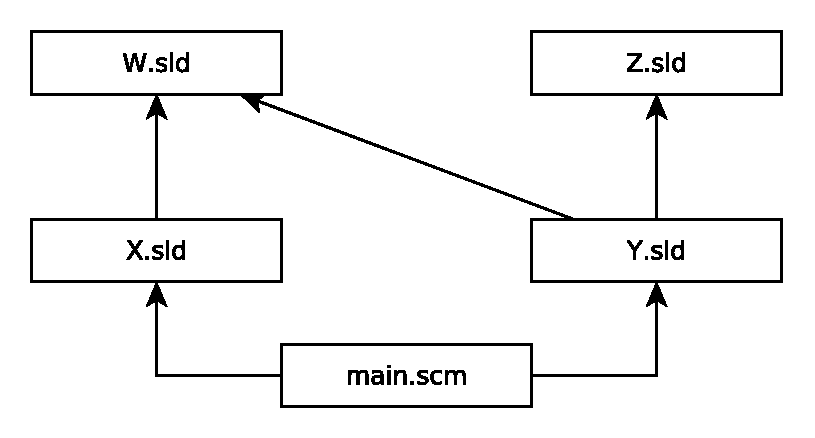
\includegraphics{figures/system-example}
  \caption{Un exemple d'un système fictif composé de différents modules.
  Le module principal se nomme \textbf{main.scm} avec l'extension \textbf{.scm}
  et les bibliothèques ont l'extension \textbf{.sld}}
  \label{fig:system-dependency-example}
\end{figure}


Dans l'exemple à la figure~\ref{fig:system-dependency-example}, l'exécution du module principal
\textbf{main.scm} déclenche la collection des modules X et Y, qui récursivement
déclenche la collection de W et Z.  L'algorithme de collection des modules gère
les modules qui apparaissent plusieurs fois au sein du graphe et les cycles.  Après la
collection de tous ces modules, le descripteur de module est
récupéré par un appel aux primitives du système d'exploitation si compilé.


\subsection{Module compilé dans Gambit}
% La construction d'un programme peut s'effectuer de façon modulaire; chaque
% composantes du programme peuvent être construites en séparément.  La
% modification d'une des bibliothèques partagés utilisés par
% le programme ne nécessite pas la recompilation de celui-ci. Le nom qui est
% donné à l'entité qui résout les noms des fonctionnalités est l'éditeur de liens (\textit{dynamic linker}).
% Habituellement les bibliothèques exportent des fonctions, mais il peuvent aussi
% exporter plusieurs types de données comme des entiers, des nombres à virgules,
% des chaînes de caractères et des données composites (structures). Chacune de ces données est
% associées à un nom unique (symbole) au sein de la bibliothèque.
% Il n'est pas possible d'avoir deux bibliothèques statiques qui exportent une
% fonctionnalité avec le même nom au sein d'une même application, alors qu'avec
% les bibliothèques partagés c'est possible. Cela limite le choix des
% bibliothèques qui peuvent être utilisé simultanément au sein du programme;
% chaque bibliothèque doit avoir un ensemble de nom de fonctionnalité distinct
% des autres. Puisque la résolution d'une fonctionnalité retourne la première
% occurrence trouvée, il n'y a rien qui empêche d'avoir plus d'une fonctionnalité
% associée au même nom.

Les modules dans Gambit peuvent être compilés pour plus de performance en
bibliothèque dynamique. Les programmes principaux peuvent être compilés en
exécutable.  Gambit permet l'utilisation de bibliothèques statiques et
dynamiques.\\

\begin{figure}[ht]
  \centering
  \lstset{language={Scheme},frame=single}

  \begin{mplisting}{0.5}
;; fib.scm
(define (fib n)
  (if (< n 2)
      n
      (+ (fib (- n 1))
         (fib (- n 2)))))
\end{mplisting}
  \caption{Un module qui implémente la fonction mathématique \texttt{fib}
    au niveau principal (<<top level>>).}
  \label{fig:basic_fib_module}
\end{figure}

La construction d'une bibliothèque dynamique à partir du fichier
\texttt{fib.scm} de la figure \ref{fig:basic_fib_module} s'effectue par le
compilateur de Gambit qui se nomme \texttt{gsc}. Cela produit
un fichier avec l'extension \texttt{.oN} où le \texttt{N} correspond au
numéro de séquence générée de la bibliothèque, qui commence à 1. Gambit support
déjà une certaine gestion des versions des modules compilés avant l'intégration
du système de module.


\section{Module hébergé}

Un module qui est hébergé est un module dont le code source est stocké sur un
serveur de versionnement de source accessible sur le réseau au nœud d'un nom
de domaine comme \url{github.com}. La syntaxe des noms de domaine est inspirée
du RFC-2396~\cite{RFC:URI-2396}.  La différence avec la spécification du
\textit{hostname} dans le RFC-2396 est que le \textit{hostname} ne peut pas se
terminer par un point et doit contenir au moins un \verb|domainlabel|. C'est
pour permettre de distinguer un module local et un module hébergé. \\

\begin{figure}[ht]
  \centering
  \lstset{frame=single}
  \begin{mplisting}{0.9}
hostname      = ( domainlabel "." )+ toplabel
domainlabel   = alphanum | alphanum ( alphanum | "-" )* alphanum
toplabel      = alpha | alpha ( alphanum | "-" )* alphanum
alphanum      = alpha | digit
alpha         = [a-zA-Z]
digit         = [0-9]
\end{mplisting}
  \caption{Grammaire EBNF représentant un hostname selon un sous-ensemble du
  RFC-2396.}
  \label{fig:hostname->grammar}
\end{figure}


\subsection{Installation automatique}
%[TODO: clarifié la whitelist]
Gambit permet l'installation automatique des modules. Pour contrôler les
provenances des modules qui sont installés automatiquement, nous avons
ajouté une liste des emplacements de confiance à l'environnement d'exécution
qui indique quels modules peuvent être installés inconditionnellement.
Nous avons nommé cette liste \textit{whitelist}, elle valide les
\textit{<module-ref>}.  La validation consiste à trouver un
élément dans la \textit{whitelist} qui correspond à un préfixe du
\textit{<module-ref>}. Chaque processus Gambit possède une
\textit{whitelist} différente, cela implique que chaque nœud Termite
peut avoir une \textit{whitelist} distinct.

%[TODO: not done, February 27 is the deadline for this part]

Un élément est considéré un préfixe, si chacune des composantes de l'élément
est incluse dans le \textit{<module-ref>} dans le même ordre. L'élément
\texttt{github.com/gambit} est un préfixe de \texttt{github.com/gambit/hello},
car les parties \texttt{github.com} et \texttt{gambit} font partie du
\textit{<module-ref>}. Le module \texttt{github.com/gambitXYZ/hello} ne
contient pas le préfixe \texttt{github.com/gambit}, car \texttt{gambit} est
différent de \texttt{gambitXYZ}.

Par défaut l'emplacement \texttt{github.com/gambit} est inclus dans la
\textit{whitelist}, puisque cela correspond à la emplacement qui de des
sources de Gambit.  Cela implique que tous les modules sous
\texttt{github.com/gambit} peuvent être installés automatiquement. Par exemple,
le module \texttt{github.com/gambit/hello} peut être installé
inconditionnellement. La \textit{whitelist} peut être modifiée par
les variables d'environnement et par les arguments de ligne de commande.

\begin{figure}[ht]
  \centering
  \fontsize{12}{7}
  \begin{mplisting}{1}
$ gsi -e '(import (github.com/feeley/pyffi))'
*** ERROR IN (stdin)@1.9 -- Cannot find library (github.com/feeley/pyffi)

$ gsi -:whitelist=github.com/feeley -e '(import (github.com/feeley/pyffi))'

$ gsi -:whitelist= -e '(import (github.com/gambit/hello))'
*** ERROR IN (stdin)@1.9 -- Cannot find library (github.com/gambit/hello)
\end{mplisting}
  \caption{Exemples de manipulation de la {\it whitelist} par
    les arguments de la ligne de commande. Le premier exemple
    montre le rejet de l'installation, car le module n'est pas dans la
    \textit{whitelist}. Le second exemple permet les modules sous
    \texttt{github.com/feeley} d'être installé automatiquement.
    Le dernier exemple montre comment désactiver l'installation automatique
    en vidant la whitelist.}
  \label{fig:whitelist_manipulation}
\end{figure}

En plus de la \textit{whitelist} nous avons aussi ajouté un mode
d'installation.  qui indique si l'installation demande une confirmation à
l'usager pour l'installation d'un module qui n'est pas dans la
\textit{whitelist}. Il y a trois modes d'installation.
\begin{itemize}
  \item \textbf{never}: il y a seulement les modules qui sont dans la
    \textit{whitelist} qui peuvent être installés.

  \item \textbf{repl} (\textit{Read Eval Print Loop}): les modules qui ne sont pas dans la \textit{whitelist}
    peuvent être installés avec la confirmation textuelle de l'usager s'il y a
    une \textit{repl} disponible. C'est le mode par défaut.

  \item \textbf{ask-always}: les modules qui ne sont pas dans la \textit{whitelist}
    peuvent être installés avec la confirmation textuelle de l'usager.
\end{itemize}

Le mode d'installation est spécifié par le \textit{runtime option} nommée
\textit{ask-install}.\\
\begin{figure}[ht]
  \lstset{language={Scheme}}
  \fontsize{12}{7}
\begin{mplisting}{1}
$ gsi -:ask-install=always
Gambit v4.9.3

> (import (github.com/frederichamel/semver))
Hosted module github.com/frederichamel/semver is required but is not installed.
Download and install (y/n)? n
*** ERROR IN (stdin)@1.9 -- Cannot find library (github.com/frederichamel/semver)
>
\end{mplisting}
  \caption{L'exemple montre le résultat d'une réponse négative lors de
    l'installation du module qui n'est pas dans la \textit{whitelist}.
    Il ne se fait pas installer.}
\end{figure}


\section{Conclusion}

Ce chapitre a traité des méthodes de chargement de module et des mécanismes
d'installation automatique qui sont requis dans la diffusion des modules.
Notre implémentation du chargement des modules garantit le chargement unique
des modules dans un ordre qui respecte les dépendances. Ceci est demandé dans
l'implémentation des modules Scheme R7RS.

Notre approche nous permet l'installation automatique de modules qui sont
inclus dans la \textit{whitelist} lorsque demandé.  Cela offre une forme simple
de contrôle de sécurité sur les modules qui peuvent s'installer automatiquement
sur un nœud du système distribué. Cela offre la diffusion des modules entre les
nœuds d'un tel système pour permettre des appels RPC sur un nœud ne connaissant
pas le code demandé.





% \subsection{Module \texttt{\_git}}

% Ce module offre un interface pour utiliser interagir avec les des dépôts git.
% Il permet de cloner un dépôts qui est hébergé sur \url{github.com}. Un clone du
% dépôts est simplement un copie qui contient les informations suffisantes pour
% passer d'une version d'un module à un autre. L'opération qui permet de changer
% de version est \emph{checkout}.


%-------------------------------------------------------------------------------
%
%Modèle "link dynamique" :
%  recherche des libs au run time, utilisation de eval (par load) et
%  load-object-file
%
%  % gsi main.scm      ou      % gsc main.scm ; gsi main.o1
%
%    origin/main.scm    : (import X Y)
%          /X/X.sld     : (import)
%
% ~~userlib/Y/Y.sld     : (import Z)
%
%     ~~lib/Z/Z.sld     : (import)
%          /Z.o1
%
%-------------------------------------------------------------------------------
%
%Modèle "link statique" :
%  recherche des libs au link time en utilisant les méta-infos
%  dans les .c (demand-lib et supply-lib), chaque .c compilé en
%  un .o séparément et les .o linkés par le compilateur C
%
%  % gsc -obj -keep-c X.sld      ;; créer .c et .o
%  % gsc -obj -keep-c Y.sld      ;; créer .c et .o
%  % gsc -obj -keep-c Z.sld      ;; créer .c et .o
%  % gsc -obj -keep-c main.scm   ;; créer .c et .o
%  % gsc -exe main.c             ;; combine les .o pour créer main.exe
%
%    origin/main.scm    : (import X Y)
%          /main.c      : (demand-lib X Y)
%          /main.o
%          /X/X.sld     : (import)
%            /X.c       : (demand-lib) (supply-lib X)
%            /X.o
%
% ~~userlib/Y/Y.sld     : (import Z)
%          /Y/Y.c       : (demand-lib Z) (supply-lib Y)
%          /Y/Y.o
%
%     ~~lib/Z/Z.sld     : (import)
%          /Z/Z.c       : (demand-lib) (supply-lib Z)
%          /Z/Z.o
%
%-------------------------------------------------------------------------------
%
%Modèle "whole-program" :
%  recherche des libs au compile time en utilisant les imports
%  dans les fichiers sources, les AST de toutes les libs fusionnées
%  en un seul AST compilé par gsc (donc un seul .c généré et compilé
%  par le compilateur C pour créer main.exe)
%
%  % gsc -exe -whole-program main.scm
%
%    origin/main.scm    : (import X Y)
%          /X/X.sld     : (import)
%
% ~~userlib/Y/Y.sld     : (import Z)
%
%     ~~lib/Z/Z.sld     : (import)
%
%-------------------------------------------------------------------------------
% correction d’une petite coquille…
% /Y.c       : (demand-lib Z) (supply-lib Y)
% /Y.o
%
% ~~lib/Z/Z.sld     : (import)
% /Z.c       : (demand-lib) (supply-lib Z)
% ...


% (check-sld "/tmp/scheme/base/base.sld" "/tmp/scheme/base")
% (check-sld "/tmp/scheme/base.sld" "/tmp/scheme")
% (check-sld
%  "/home/frederic/Documents/MasterResearch/gambit9/lib/cocolappin/scheme/base/base.sld"
%  "/home/frederic/Documents/MasterResearch/gambit9/lib/cocolappin/scheme/base")
% (check-sld
%  "/home/frederic/Documents/MasterResearch/gambit9/lib/cocolappin/scheme/base.sld"
%  "/home/frederic/Documents/MasterResearch/gambit9/lib/cocolappin/scheme")
% (check-sld
%  "/home/frederic/Documents/MasterResearch/g9/lib/scheme/base/base.sld"
%  "/home/frederic/Documents/MasterResearch/g9/lib/scheme/base")
% object-file-path: /home/frederic/Documents/MasterResearch/g9/lib/scheme/base/.gambit_409003@C/base.o1
% ("/home/frederic/Documents/MasterResearch/g9/lib/scheme/base/base.sld"
%  .
%  #<input-port #2 "/home/frederic/Documents/MasterResearch/g9/lib/scheme/base/base.sld">)


\chapter{Gestion des modules}
\label{ch:module_management}

% TODO: too much detail in intro
%       il ne faut pas faire un sommaire du carteau du chapitre, mais motiver
%       l'existance de ce chapitre
%       et mentionner ce dont tu va parler et pourquoi (le lien avec ce travail)

Ce chapitre décrit l'organisation des modules sur le système de fichier pour
permettre plusieurs versions d'un module. Notre approche est d'associer à
chaque version d'un module un répertoire différent. Cela permet de stocker les
différentes versions d'un module dans le système de fichier.  Nous avons
comparé les différentes façons d'organiser les modules dans plusieurs langages
comme Python, JavaScript, Go, OCaml. Il est important que l'installation d'un
module n'altère pas la stabilité des autres modules.  Le modèle de gestion des
modules choisi garantit que les dépendances d'un module sont fixes.

\section{Sommaire}
% Installation, Désinstallation, Mise à jour, Compilation/Exécution
La gestion des modules inclut généralement l'installation, la mise à jour et
la désinstallation. L'organisation des modules est un élément important
dans la gestion des modules. Les gestionnaires de modules sont présents dans
beaucoup de langages tels que Python, Ruby, JavaScript, Common Lisp, Go, etc.
Un gestionnaire de module est inclus dans le système Gambit Scheme pour
organiser les modules.

Le gestionnaire de module de Gambit Scheme fournit les opérations
d'installation, de désinstallation, de mise à jour, de compilation
d'un module et l'exécution des tests unitaires du module. Les modules
sont versionnés par Git. L'emplacement des modules est spécifié par
une liste de répertoires qui inclut les modules système et les modules
utilisateur. La gestion des modules est effectuée par le module \lstcode{_pkg}
qui offre les procédures d'installation d'installation et de désinstallation.


% % quicklisp.org
% Les gestionnaires de module permettent plusieurs opérations sur les modules
% comme l'installation, la mise à jour et la désinstallation. La gestion inclut
% l'organisation des versions des modules sur le système de fichier. Beaucoup de
% de langages ont au moins un gestionnaire de modules. Le langage Python a le
% gestionnaire de module \textbf{pip}. L'implémentation NodeJS pour Javascript à
% le gestionnaire de module \textbf{npm}. Le langage Common Lisp a le gestionnaire
% \textit{quicklisp}.

% Les gestionnaires de module utilisent une hiérarchie de répertoires pour
% organiser les modules. Il existe plusieurs façon pour gérer les modules.
% Certain permette plusieurs versions d'un module dans un même environnement,
% comme dans le langage Go.

% Les module Gambit sont situés dans des répertoires spécifié dans le
% \lstcode{search-order}. Par défaut, il y a un répertoire pour les modules
% systèmes\ref{modules_systems} et un répertoire pour les modules
% utilisateurs\ref{modules_utilisateurs}. Ces répertoires sont associés au
% répertoire d'installation de Gambit. Les répertoires d'installation sont
% dénotés par un préfixe \lstcode{\~\~}.  Le modules système utilise utilise par
% défaut le répertoire d'installation \lstcode{\~\~lib} alors que les modules
% utilisateurs utilise le répertoire \lstcode{\~\~userlib}. Chaque module peut
% être installé, désinstallé, testé et compilé. La plupart de ces opérations est
% faite par le module gambit \lstcode{_pkg}.  Il est possible d'invoquer ces
% opérations par des arguments de ligne de commande passé à Gambit.

\section{Organisation des modules}

Les modules sont organisés dans des répertoires donnés par le système Gambit.
Ils contiennent l'ensemble des modules internes et actuellement installés sur
le système. Il y a trois principaux répertoires spéciaux qui contiennent des
modules.

\begin{itemize}
  \item \lstcode{\~\~userlib}: c'est le répertoire qui contient les modules
    de l'utilisateur, par défaut \texttt{.gambit\_userlib} dans le répertoire
    maison de l'utilisateur.

  \item \lstcode{\~\~lib}: c'est le répertoire d'installation de Gambit
    qui contient les modules système. Les modules dans ce répertoire sont
    communs à tous les utilisateurs.

  \item \lstcode{\~\~instlib}: c'est le répertoire d'installation des modules.
    Par défaut, il correspond au répertoire \lstcode{\~\~userlib}.
\end{itemize}

Un module local ou hébergé est identifié de façon unique par un
\lstcode{module-ref}.  Un \lstcode{module-ref} est séparé en trois parties: le
\lstcode{hostname}, le \lstcode{path} et l'étiquette qui donne la version.  La
différence entre une référence à un module local et hébergé est la première
partie. Dans le cas hébergé, le champ \lstcode{hostname} contient
l'information du nom de domaine qui, dans le cas local, est vide.
Le \lstcode{<tag>} spécifie la version du module avec une référence à
un commit du système de révision Git. Un \lstcode{<tag>} vide réfère
à la version de développement du module.  La syntaxe du
nom de domaine est donnée par la grammaire[\ref{lst:hostname->grammar}].  La
grammaire formelle\ref{lst:module-ref->grammar} décrit la syntaxe du
\lstcode{<module-ref>} dans le cas hébergé et local.\\

\begin{figure}[ht]
  \lstset{frame=single}
  \begin{mplisting}{0.8}
<module-ref> := <local> | <hosted>
<local>      := <id>(/<id>)*<tag>
<hosted>     := <hostname>/<id>/<id>(/<id>)*(@<tag>)?
\end{mplisting}
  \caption{Grammaire formelle}
  \label{lst:module-ref->grammar}
\end{figure}

Le \lstcode{module-ref} \lstcode{github.com/gambit/hello} réfère
au module \lstcode{hello} sur le serveur de révision \lstcode{github.com}
dans l'espace \lstcode{gambit}. Le champ \lstcode{host} est dans ce
cas \lstcode{github.com/gambit} qui correspond au nom de domaine avec
le nom de l'espace sur le serveur.

% \begin{itemize}
%   \item \lstcode{install} effectue l'installation de modules.
%   \item \lstcode{update} effectue la mise à jour de la cache des modules demandés. Cela
%     permet d'actualiser les nouvelles versions disponible d'un module.
%   \item \lstcode{uninstall} désinstalle les modules spécifié.
%   \item \lstcode{test} exécute les tests unitaires des modules spécifiés.
% \end{itemize}

\subsection{Installation de module}
L'installation des modules peut être soit à partir d'un serveur de révision
ou d'un répertoire local versionné par git. Dans les deux cas d'installation,
le \lstcode{module-ref}  est utilisé pour déterminer l'emplacement du module
dans le répertoire des modules. Chaque \lstcode{module-ref} est associé à un
répertoire unique dans le répertoire des modules.

% Les modules qui sont hébergés sur un serveur de révision comme github, gitlab, bitbucket,
% etc ont un \lstcode{module-ref} distinct.

% L'organisation des module doit permettre l'installation de plusieurs
% version d'un même module. C'est pour cela qu'il sont organisés dans une
% hiérarchie de répertoire lié au \lstcode{module-ref} du module.
% Chaque version d'un module est identifié par un seul \lstcode{module-ref}
% qui est associé à un seul emplacement sur le système de fichier.

% L'organisation des répertoires des modules permet l'installation de plusieurs
% versions d'un même module. Cela garantie que tous les modules qui utilise une
% version antérieur de modules fonctionne toujours. Certains systèmes de module
% ne conserve qu'une seul version de chaque module. La mise à jour d'un module
% peut briser le fonctionnement de ses dépendances.

% Les versions des modules sont lié au publications des module sur les serveurs
% de version tels que que github, gitlab, bitbucket, etc. Une versions est soit
% une branche ou un étiquette. Les versions sont spécifier par un \lstcode{@}
% suivie de la version. Par exemple, la version \lstcode{1.0.0} est notée le
% suffixe \lstcode{@1.0.0}.


Les modules sont hébergés sur des serveurs de version tels que github, gitlab,
bitbucket, etc. Chaque version d'un module est installée dans un répertoire
distinct. Il est donc possible d'avoir plus d'une version d'un module installé.
L'installation des modules s'effectue par l'intermédiaire du module
\lstcode{_git} qui offre une interface à l'utilitaire \lstcode{git}. Le
processus d'installation est séparé en plusieurs étapes.  Le contenu du module
est installé dans un répertoire temporaire qui est ensuite renommé au
répertoire de destination. Cela permet d'installer le module de façon atomique.

Tout d'abord, la
branche \lstcode{master} du dépôt du module est clonée. Ensuite, une archive de la
version est faite et extraite dans le préfixe des modules. Le préfixe est par
défaut \lstcode{\~\~userlib}.  Il est possible de spécifier un préfixe
d'installation dans lequel installer les modules. Plusieurs versions d'un même
module coexistent dans le même préfixe d'installation.

La branche \lstcode{master} est utilisée comme version de développement et
comme cache pour installer les autres versions. Une version d'un module est soit
un \textit{commit}, une branche ou une étiquette. L'installation d'une version
spécifique utilise la cache pour récupérer l'archive de la version demandée
et l'extraire dans l'espace des modules.

La procédure \lstcode{install} de \lstcode{_pkg} accepte deux paramètres:
le nom du module et de façon optionnelle le préfixe d'installation. Elle
retourne la valeur de vérité vraie (\lstcode{#t}) si l'installation réussit,
sinon elle retourne fausse (\lstcode{#f}).
\begin{center}
  \begin{mplisting}{0.4}
(install mod #!optional to)
\end{mplisting}
\end{center}

L'installation peut être effectuée en passant l'option \lstcode{-install}
à l'interprète gambit. Cette option requiert le nom du module et
de façon optionnelle le préfixe d'installation.
\begin{center}
  \begin{mplisting}{0.8}
$ gsi -install [-to <path>] module [...]
\end{mplisting}
\end{center}
Le préfixe \lstcode{<path>} est la racine utilisée pour installer les modules
et est spécifié par l'option \lstcode{-to}.  La racine par défaut est
\lstcode{\~\~userlib}. Voici un exemple d'installation d'une version spécifique du module
\lstcode{semver} qui implémente la logique du \textit{semantic versioning}.

\begin{center}
  \begin{mplisting}{1}
$ gsi -install -to /tmp/exemple github.com/frederichamel/semver@1.0.1
\end{mplisting}
\end{center}

\section{Désinstallation}

La désinstallation d'un module consiste à supprimer les fichiers
de ce module. Le module \lstcode{_pkg} offre la procédure
\lstcode{uninsall} qui accepte deux arguments: le nom du module,
et de façon optionnelle, le répertoire dans lequel les modules
sont situés. Les valeurs retournées par cette procédure sont
similaires à la procédure.
\begin{center}
  \begin{mplisting}{0.4}
(uninstall mod #!optional to)
\end{mplisting}
\end{center}
La désinstallation peut être faite en passant l'option \lstcode{-uninstall}
à l'interprète Gambit. Cette option requiert le nom du module et le
répertoire  des modules à désinstaller.
\begin{center}
  \begin{mplisting}{0.8}
$ gsi -uninstall [-to <path>] module
\end{mplisting}
\end{center}
Le répertoire \lstcode{<path>} est l'emplacement des modules
à désinstaller. Le format des arguments pour la désinstallation
est le même que pour l'installation. Le répertoire par défaut
est le répertoire \lstcode{\~\~userlib}.

La désinstallation du module \lstcode{semver} qui est installé dans
le répertoire \lstcode{/tmp/exemple} est fait par la commande suivante:
\begin{center}
  \begin{mplisting}{1}
$ gsi -uninstall -to /tmp/exemple github.com/frederichamel/semver@1.0.1
\end{mplisting}
\end{center}


\section{Mise à jour}
Cette opération actualise la branche \lstcode{master} du module.
Cela donne accès aux nouvelles publications d'un module. Pour installer
une nouvelle version d'un module, il suffit de faire la mise à jour
de la branche master et d'installer la nouvelle version.

\begin{center}
  \begin{mplisting}{0.8}
$ gsi -update [-to <path>] module
\end{mplisting}
\end{center}

\section{Tests unitaires}
Les tests unitaires exécutés sont dans un fichier conjoint au module.
Gambit offre un module de test unitaire nommé \lstcode{_test}. Il
contient plusieurs procédures et macros pour tester le bon fonctionnement d'un module.
Les tests unitaires pour un module nommé \lstcode{A} sont dans le sous-module
\lstcode{A/test}.

\begin{center}
\begin{mplisting}{0.8}
$ gsi module/test
*** all tests passed out of a total of %*\textit{N}* tests
\end{mplisting}
\end{center}

La commande affiche le résultat des tests unitaires contenus dans le
sous-module test.

% Exemple de tests.

\section{Compilation d'un module}
%
La compilation d'un module est faite en passant le nom du module
(\texttt{\textit{<module-ref>}}) en paramètre.  Le compilateur cherche le
module dans les répertoires du \lstcode{##module-search-order}. Le module est
installé au besoin et ensuite compilé dans un sous répertoire. Ce dossier associe
la compilation de ce module à la version de Gambit et à la cible (C, JavaScript, \dots).
La compilation d'un module se fait par la commande suivante:

\begin{center}
\begin{mplisting}{0.8}
$ gsc %*\textit{<module-ref>}*
\end{mplisting}
\end{center}

%% Module avec du C.
L'arborescence du répertoire du module après la compilation du module
\texttt{\_digest} pour le \textit{backend} C ressemble à:
%
\begin{center}
\begin{mplisting}{0.8}
|-- _digest@gambit409003@C
|   |-- _digest.c
|   `-- _digest.o1
|-- _digest#.scm
|-- _digest.scm
`-- test.scm

1 directory, 5 files
\end{mplisting}
\end{center}


\section{Comparaison avec d'autre système}

L'organisation des modules sur le système de fichier dans Gambit
diffère de celui de OCaml, Python et NodeJS. Ceux-ci ne permettent pas
l'installation de plus d'une version d'un module directement. Le système
de module qui est utilisé dans le langage de programmation Go est le plus
similaire à celui dans Gambit.

Un système de module permet la coexistence de plusieurs versions du même module
sur le système de fichier s'ils sont considérés comme des modules différents.
L'installation d'une version différente d'un module ne remplace pas la version
déjà installée. L'organisation des bibliothèques est importante pour permettre
cette coexistence.

La caractéristique que le système de bibliothèque doit avoir pour permettre
plusieurs versions d'une bibliothèque est une organisation qui permet de
distinguer les différentes versions de la bibliothèque par un chemin unique.
La plupart des systèmes de module ne distinguent pas les versions d'un même
module et ne permettent l'installation que d'une seule version. Les systèmes de
module permettent la gestion de différents préfixes dans lesquels les modules sont
installés. Chaque préfixe peut contenir une version différente d'un même
module. Pour avoir une nouvelle version d'un module, il faut créer un nouveau
préfixe.


%Le nombre de bibliothèque moyen dans un langage est d'environ 90000 \colorbox{red}{ref}
%en prennant en compte les gestionnaire de modules (bibliothèques) suivant:

% \todo{Include number of module in pm from www.modulecounts.com}

% Il est à noté que le nombre de bibliothèques qu'un langage possède est lié au nombre
% d'utilisateur. Aussi le nombre de bibliothèques n'est pas représentatif du nombre
% réellement utilisé.

\begin{figure}[h]
\begin{tabular}{|r|c|c|c|c|}
  \hline   & Multiple versions \\\hline
  OCaml    & \xmark            \\\hline
  Python   & \xmark            \\\hline
  NodeJS   & \xmark            \\\hline
  Java     & \xmark            \\\hline
  Go       & \checkmark        \\\hline
%  Gambit Scheme & \checkmark & \checkmark & default \\\hline
\end{tabular}

\caption{Une table qui compare différents systèmes de module sur la capacité
  d'installer plusieurs versions d'un module.  Le système Go permet plusieurs
  versions d'un module pour des versions incompatibles selon le sémantique de
  version. La version \texttt{1.0.0} coexiste avec la version \texttt{2.0.0}.
  La version récente \texttt{1.2.0} remplace la vieille version \texttt{1.0.1}.}

\end{figure}




%\subsubsection{Organisation dans Gambit Scheme}
%\todo{}
% exemple coexistence sur un système de fichier

\subsection{Organisation de OCaml}
%
Le système de gestion de bibliothèques d'OCaml se nomme OPAM. Ce système permet
d'avoir plusieurs environnements distincts contenant chacun un ensemble de
versions des bibliothèques.  Chaque environnement permet l'installation d'une
version spécifique de chaque bibliothèque et est étiqueté avec un nom choisi
par l'utilisateur. Un changement d'environnement est effectué par une requête
de l'utilisateur \verb|opam switch <envname>|. Il utilise le projet
\textit{mancoosi} pour gérer les contraintes de
version, les dépendances optionnelles et la gestion des conflits.
L'environnement par défaut est lié aux dépôts standard d'OCaml.

\subsection{Organisation de Python}
%
L'organisation des bibliothèques Python ne permet de stocker que la dernière
version d'une bibliothèque. Les emplacements des bibliothèques sont modifiés
par la variable d'environnement \verb|PYTHONPATH| qui correspond dans Python à
la variable \verb|path| de la bibliothèque interne \verb|sys|. Le système de
bibliothèque de Python ne permet pas la coexistence de plusieurs versions de la
même bibliothèque. Le \textit{package manager} principal de Python est
\textit{pip}.  L'installation d'une autre version d'une bibliothèque
désinstalle ou masque la version déjà installée. Le système de module ne permet
pas de référer à deux versions de la même bibliothèque.

\begin{figure}[ht]
    \begin{minipage}[t]{0.5\textwidth}
\begin{verbatim}
>>> import sys
>>> print('\n'.join(sys.path))
/usr/lib/python37.zip
/usr/lib/python3.7
/usr/lib/python3.7/lib-dynload
/home/username/.local/lib/python3.7/site-packages
/usr/lib/python3.7/site-packages
\end{verbatim}
    \end{minipage}
    \caption{L'ensemble des répertoires qui est utilisé par Python version 3.7
    pour organiser les bibliothèques sur un système de type Linux.}
\end{figure}

Python a le concept équivalent à OCaml de \textit{virtualenv} qui permet
d'avoir plusieurs versions installées sur la même machine. Cela permet
d'installer des bibliothèques dans un environnement isolé des autres.
L'avantage est qu'il est possible d'avoir une compatibilité avec des logiciels
qui utilisent des versions de bibliothèques antérieures. Un inconvénient est
qu'il n'y a pas un partage des versions de bibliothèques communes entre les
différents environnements, cela a comme effet d'avoir plus d'un exemplaire d'une
version de la bibliothèque installée sur le système de fichier. Chaque
\texttt{virtualenv} ne permet qu'une seule version de chaque bibliothèque
d'être installé.

%\todo{\hspace{2.5in}Image de coexistence venv}

\subsection{Organisation de NodeJS}
%
NodeJS est un interprète JavaScript qui a été conçu pour être exécuté du côté
serveur dans un modèle client-serveur. Les bibliothèques sont installées au
niveau du projet. Cela implique que plusieurs projets qui utilisent la même
version de la bibliothèque vont référer au même exemplaire de la
bibliothèque.

La structure d'une bibliothèque dans NodeJS est décrite par un fichier
\texttt{package.json} qui contient plusieurs méta données comme
le nom, la version, le nom des dépendances, la version des dépendances,
la licence sous laquelle la bibliothèque est publiée et plusieurs autres
méta données liées à la bibliothèque. Sous NodeJS, les bibliothèques sont gérées
par projet plutôt que globalement cela a comme avantage que chaque projet
fonctionne avec ses versions des bibliothèques.

\subsection{Organisation de Java}
%
Les modules en Java sont nommés \textit{package}.  Le nom des modules utilise
généralement l'inverse d'une URL comme espace de nom. Par exemple, les noms des
modules liés aux services Google vont débuter par \texttt{com.google}. Cette
convention a pour but d'unifier les noms de module. La version des modules
n'est pas liée au nom du module dans le cas de Java. Il n'est pas possible de
charger deux modules qui utilisent le même espace de nom, comme deux versions
d'un même module.

\subsection{Organisation de Go}
%
L'organisation des bibliothèques dans Go~\cite{GoLang} est plus dans un contexte
environnement dont la racine est spécifiée par la variable d'environnement
\texttt{GOPATH} avec un répertoire pour les exécutables compilés
(\texttt{bin}), un répertoire contenant le code source des différents projets
(\texttt{src}) et un répertoire pour les objets des modules installés
(\texttt{pkg}). Chaque paire de systèmes d'exploitation et d'architecture a son
propre répertoire dans \texttt{pkg}.

Le système Go permet l'installation de plusieurs versions d'un même module dans
le même environnement en utilisant le service \textit{gopkg.in}. Il y a deux
syntaxes utilisées pour l'URL des modules Go avec \textit{gopkg.in}. Il est possible
de spécifier une version spécifique du module lors de l'importation.

\noindent
\begin{figure}[ht]
  \centering
\begin{mplisting}{1}
gopkg.in/pkg.v3      -> github.com/go-pkg/pkg (branch/tag v3, v3.N, or v3.N.M)
gopkg.in/user/pkg.v3 -> github.com/user/pkg   (branch/tag v3, v3.N, or v3.N.M)
\end{mplisting}
  \caption{Exemple d'importation de la version v3 du module pkg en utilisant
    le service \textit{gopkg.in}.}
  \label{fig:gopkg_import}
\end{figure}

\begin{figure}[h]
  \lstset{language={Go},frame=single}
\begin{mplisting}{1}
package main

import (
  hellov1 "gopkg.in/FredericHamel/go-hello.v1"
  hellov2 "gopkg.in/FredericHamel/go-hello.v2"
)

func main() {
  // use hello version 1
  hellov1.Hello("Bob")

  // use hello version 2
  hellov2.Salut("Alice")

  // hellov1.Salut("Eve")
}
\end{mplisting}
  \caption{Un exemple qui montre l'importation de deux versions d'un même module
    en Go. Le module \textbf{go-hello} version 2 exporte la fonction \texttt{Salut}
    qui n'existe pas dans la version \texttt{1}.}
\end{figure}

% https://labix.org/gopkg.in
% go help importpath

%La structure du répertoire dans un projet g
\begin{figure}[ht]
  \centering
  \lstset{frame=single}
\begin{mplisting}{1}
$GOPATH/
  - bin
    - ... binaries
  - src
    - github.com
      - UserName1
        - project1
        - project2
      - UserName2
        - projectA
        - projectB
  - pkg
    - linux_amd64
      - pkglist
        - objets
\end{mplisting}
  \caption{Arborescence des fichier dans le gopath.}
  \label{fig:organisation_go}
\end{figure}

\section{Conclusion}
%
Ce chapitre a traité de la gestion des modules.  Les opérations du système de
modules présentés dans ce chapitre sont l'installation, la désinstallation et
la mise à jour.  Notre approche de gestion des modules offre correctement la
possibilité d'avoir plus d'une version d'un module. Cela empêche les bris de
dépendances lors de l'installation de nouveaux modules.  L'installation des
modules peut-être déclenchés procéduralement ce qui est nécessaire pour diffuser
les modules.

Il est possible de forcer la compilation d'un module par la présence d'un fichier
\textit{module-name.\_must-build\_}. Cette fonctionnalité permet le chargement d'un
module qui doit être compilé pour fonctionner.



\chapter{Gestion des modules}
\label{ch:module_management}

Gambit utilise deux répertoires principaux pour les modules.  Ils sont associés
aux alliasses de répertoire \lstcode{\~\~userlib} et \lstcode{\~\~lib} qui
correspond aux emplacements respectifs des modules utilisateurs et des modules
systèmes. Les différents opérations sont l'installation de modules, la mise à
jour des modules, la désinstallation de modules, l'exécution des tests
unitaires et la compilation. La gestion des modules est faite par le module
\lstcode{gambit/pkg}. Il est possible d'invoquer ces opérations par des
arguments de ligne de commande passé à Gambit.

% \begin{itemize}
%   \item \lstcode{install} effectue l'installation de modules.
%   \item \lstcode{update} effectue la mise à jour de la cache des modules demandés. Cela
%     permet d'actualiser les nouvelles versions disponible d'un module.
%   \item \lstcode{uninstall} désinstalle les modules spécifié.
%   \item \lstcode{test} exécute les tests unitaires des modules spécifiés.
% \end{itemize}

L'organisation des répertoires des modules permet l'installation de plusieurs
versions d'un même module. Cela garantie que tous les modules qui utilise une
version antérieur de modules fonctionne toujours. Certains systèmes de module
ne conserve qu'une seul version de chaque module. La mise à jour d'un module
peut briser le fonctionnement de ses dépendances.

Les versions des modules sont lié au publications des module sur les serveurs
de version tels que que github, gitlab, bitbucket, etc. Une versions est soit
une branche ou un étiquette.

% TODO: test if branch work

\section{Installation}

Les modules sont hébergés sur des serveurs de version tel que github, gitlab,
bitbucket, etc. L'installation des modules s'effectue par l'intermédiaire de
\lstcode{git}. Un module est installé en plusieurs étapes. Tout d'abord, la
branche \lstcode{master} dépôt du module est cloné. Ensuite un archive de la
version est faite et extraite dans le préfixe des modules. Le préfixe est par
défaut \lstcode{\~\~userlib}.  Il est possible de spécifier un préfixe
d'installation dans lequel installer les modules. Plusieurs versions d'un même
module coexistent dans le même préfixe d'installation.

La branche \lstcode{master} est utilisé comme version de développement et
comme cache pour installer les autres versions. Une version d'un module est soit
un commit une branche ou un étiquette. L'installation d'une version
spécifique utilise la cache pour récupérer l'archive de la version demandé
et l'extraire dans l'espace des module.

La procédure \lstcode{install} de \lstcode{gambit/pkg} accepte deux paramètres:
le nom du module et de façon optionnelle le préfixe d'installation. Elle
retourne la valeur de vérité vrai (\lstcode{#t}) si l'installation réussi,
sinon faux (\lstcode{#f}).
\begin{center}
  \begin{mplisting}{0.4}
(install mod #!optional to)
\end{mplisting}
\end{center}

L'installation peut être effectué en passant l'option \lstcode{-install}
à l'interprète gambit. Cette option requière le nom du module et
de façon optionnelle le préfixe d'installation.
\begin{center}
  \begin{mplisting}{0.8}
> gsi -install [-to <path>] module [...]
\end{mplisting}
\end{center}
Le préfixe \lstcode{<path>} est la racine utilisée pour installer les modules
et est spécifier par l'option \lstcode{-to}.  La racine par défaut est
\lstcode{\~\~userlib}. Voici un exemple d'installation d'une version spécifique du module
\lstcode{semver} qui implémente la logique du \textit{semantic versioning}.

\begin{center}
  \begin{mplisting}{1}
> gsi -install -to /tmp/exemple github.com/frederichamel/semver/tree/1.0.1
\end{mplisting}
\end{center}

\section{Désinstallation}

La désinstallation d'un module consiste à supprimer les fichier
de ce module. Le module \lstcode{gambit/pkg} offre la procédure
\lstcode{uninsall} qui accepte deux arguments: le nom du module
et de façon optionnelle le répertoire dans lequel les modules
sont situé. Les valeurs retournées par cette procédure sont
similaire à la procédure.
\begin{center}
  \begin{mplisting}{0.4}
(uninstall mod #!optional to)
\end{mplisting}
\end{center}
La désinstallation peut être fait en passant l'option \lstcode{-uninstall}
à l'interprète Gambit. Cette option requière le nom du module et le
répertoire  des module à désinstaller.
\begin{center}
  \begin{mplisting}{0.8}
> gsi -uninstall [-to <path>] module
\end{mplisting}
\end{center}
Le répertoire \lstcode{<path>} est l'emplacement des module
à désinstallé. Le format des arguments pour la désinstallation
est le même que pour l'installation. Le répertoire par défaut
est le répertoire \lstcode{\~\~userlib}.

La désinstallation du module \lstcode{semver} dans installé dans le
répertoire \lstcode{/tmp/exemple} est fait par la commande suivante:
\begin{center}
  \begin{mplisting}{1}
> gsi -uninstall -to /tmp/exemple github.com/frederichamel/semver/tree/1.0.1
\end{mplisting}
\end{center}


\section{Mise à jour}
Cette opération actualise la branche \lstcode{master} du module.
Cela donne accès au nouvelle publication d'un module. Pour installer
une nouvelle version d'un module, il suffit de faire la mise à jour
de la branche master et d'installer la nouvelle version.

\begin{center}
  \begin{mplisting}{0.8}
> gsi -update [-to <path>] module
\end{mplisting}
\end{center}

\section{Tests unitaires}
Les tests unitaires exécutés sont dans dans un fichier conjoint au module.
Gambit offre un module de test unitaire nommé \lstcode{gambit/test}. Il
contient plusieurs procédure pour tester le bon fonctionnement d'un module.
Les tests unitaires pour un module nommé \lstcode{A} est un fichier
\lstcode{A-test.scm} dans le répertoire du module.

\begin{center}
  \begin{mplisting}{0.8}
> gsi -test [-to <path>] module
\end{mplisting}
\end{center}

La commande de test ci-dessus réussi si l'exécution des teste termine sans
lancer d'erreurs.

% Exemple de tests.

\section{Compilation d'un module}
Il n'y a pas d'options spécial pour demander la compilation d'un module.
Il suffit d'invoquer le compilateur de Gambit avec le nom du module
à compiler. Le nom du module est le même que celui utilisé dans la
l'importation.

%% Module avec du C.




\chapter{Évaluation}

Ce chapitre évalue les performances du système de modules.  Notre approche
d'évaluation utilise trois programmes de test (benchmarks). Nous avons
fait des expérimentations pour comparer les performances de la diffusion de
module, que nous avons conçu, dans un contexte compilé avec la diffusion
de code interprété déjà présent dans Termite Scheme.

Le but est de prouver que l'utilisation de modules compilés, rendu possible par
notre approche, est plus avantageuse au niveau de la performance par rapport à
la diffusion de code interprété. Nous avons aussi testé la diffusion des modules
entre des nœuds de nature différente (ARM, x86).

% de taille
% différente. Nous les avons adaptés pour qu'ils testent la diffusion des
% modules. Les éléments évalués sont le temps d'exécution complet, le temps de
% compilation Scheme vers C, le temps de compilation du code C, le temps
% d'installation des modules, le temps de transfert et le temps d'exécution du
% benchmark.

% L'hypothèse est que les temps d'exécution, de compilation,
% d'installation et de transfert dépendent de la taille du module de
% test.

% Nous avons comme hypothèse que le temps d'exécution global des tests est plus
% rapide lorsque compilé qu'interprété. L'interprétation d'un programme a un coût en
% temps.

\section{Description des expériences}

% NOTE: distingué version .oN et version du code.
Les expériences exploitent l'installation automatique des modules pour la
diffusion.  Les performances du système de module sont mesurées en utilisant le
temps de téléchargement, de compilation et de chargement des modules. Les
modules pour tester les capacités de diffusion de code sont basés sur certains
\textit{benchmarks} standard de Scheme présent dans Gambit:

\begin{itemize}
  \item Puzzle (4K)
  \item Scheme (40K)
  \item Compiler (400K)
\end{itemize}

Nous référons à ces \textit{benchmarks} par leur taille du code source
(4K, 40K et 400K).

Les tests de performance sont effectués sur deux nœuds \textbf{A}
et \textbf{B}. Le test de rpc consiste à diffuser une tâche
sur le nœud générique \textbf{B}. Le nœud générique ne connait aucun
code qui est diffusé dessus.

La diffusion de code est effectuée 100 fois pour chaque benchmark. Le temps
d'exécution du benchmark est paramétré de telle sorte que le temps de la version
interprétée du benchmark soit proportionnel à sa taille. Le temps respectif de
la version interprétée des benchmarks Puzzle, Scheme et Compiler sont
respectivement dans les ordres de 0.1 seconde, 1 seconde et 10 secondes. La
figure~\ref{fig:gambit-arctic-interp} montre cette tendance dans les temps
d'exécutions. Notre but est de montrer un lien entre la taille du
programme et le temps d'exécution.

\section{Spécification des machines}
Les machines sur lesquelles les tests ont été effectués sont:
\begin{itemize}
  \item arctic, une machine \texttt{x86\_64} roulant Linux;
  \item gambit, une machine \texttt{x86\_64} roulant macOS;
  \item tictoc, un Raspberry Pi \texttt{ARM} roulant Linux.
\end{itemize}

Les spécifications détaillées de ces machines sont présentes à
l'annexe~\ref{ch:annexeA}. La diversité des machines utilisées montre que la
diffusion de code compilé est indépendante de la plateforme et de l'architecture de la
machine.

La machine \textbf{arctic} est la machine la plus stable de toutes
celles utilisées, car elle a un système de refroidissement au liquide.

\section{Résultats}

Les temps dans les tests sont mesurés en millisecondes (ms).  Les éléments qui
affectent les résultats sont le réseau et la vitesse de la machine de
destination. Ètant donnée que le réseau a affecté 10\% des transmissions
effectuées dans l'ensemble des tests dans l'ordre des millisecondes, nous avons
enlevé 5\% des valeurs minimales et 5\% des valeurs maximales.  Cela est
observé par une variance élevée dans le temps de transfert.  Pour la même
taille de transmission, le temps de transfert est plus grand pour plusieurs
exécutions.

\begin{figure}[ht]
  \centering
\begin{tabular}{|l|r|r|r|}
\hline & 4K & 40K & 400K\\\hline
Temps total & $~~~~~150.9(\sigma = ~~1.4)$ & $~~~~~978.2(\sigma = ~~1.5)$ & $~~~12397.7(\sigma = ~~5.2)$\\\hline
%Serialization & $~~~~~~~0.2(\sigma = ~~0.0)$ & $~~~~~~~0.2(\sigma = ~~0.0)$ & $~~~~~~~0.1(\sigma = ~~0.0)$\\\hline
%Deserialization & $~~~~~~~5.2(\sigma = ~~0.0)$ & $~~~~~~10.6(\sigma = ~~0.0)$ & $~~~~~~46.7(\sigma = ~~1.0)$\\\hline
%Transmission & $~~~~~~~0.4(\sigma = ~~0.0)$ & $~~~~~~~0.7(\sigma = ~~0.0)$ & $~~~~~~~7.7(\sigma = ~~0.1)$\\\hline
Transfert & $~~~~~~~5.8(\sigma = ~~0.0)$ & $~~~~~~11.6(\sigma = ~~0.0)$ & $~~~~~~54.6(\sigma = ~~1.0)$\\\hline
Exécution & $~~~~~139.0(\sigma = ~~1.3)$ & $~~~~~957.3(\sigma = ~~1.3)$ & $~~~12274.7(\sigma = ~~5.0)$\\\hline
\end{tabular}
  \caption{Comparaison de la performance RPC de Termite avant les modules dans un contexte interprété sur
    la machine Gambit. (temps en millisecondes)}
  \label{fig:gambit-arctic-interp}
\end{figure}

\begin{figure}[ht]
  \centering
\begin{tabular}{|l|r|r|r|}
\hline & 4K & 40K & 400K\\\hline
RPC & $~~~~~178.6(\sigma = ~~1.4)$ & $~~~~1033.0(\sigma = ~~1.8)$ & $~~~12871.0(\sigma = ~18.5)$\\\hline
%Serialization & $~~~~~~~0.2(\sigma = ~~0.0)$ & $~~~~~~~0.2(\sigma = ~~0.0)$ & $~~~~~~~0.1(\sigma = ~~0.0)$\\\hline
%Deserialization & $~~~~~~~5.2(\sigma = ~~0.0)$ & $~~~~~~10.9(\sigma = ~~0.0)$ & $~~~~~~33.9(\sigma = ~12.5)$\\\hline
%Transmission & $~~~~~~~1.1(\sigma = ~~0.2)$ & $~~~~~~~1.9(\sigma = ~~0.3)$ & $~~~~~~16.3(\sigma = ~~4.8)$\\\hline
Transfert & $~~~~~~~6.6(\sigma = ~~0.2)$ & $~~~~~~13.1(\sigma = ~~0.3)$ & $~~~~~~50.4(\sigma = ~13.6)$\\\hline
Execution & $~~~~~154.3(\sigma = ~~1.1)$ & $~~~~~987.1(\sigma = ~~1.5)$ & $~~~12559.9(\sigma = ~~4.6)$\\\hline
\end{tabular}
  \caption{Comparaison de la performance RPC de Termite avant les modules dans un contexte interprété sur
    la machine Tictoc. (temps en millisecondes)}
  \label{fig:tictoc-arctic-interp}
\end{figure}

\begin{figure}[ht]
\centering
\begin{tabular}{|l|r|r|r|}
\hline & 4K & 40K & 400K\\\hline
Temps total & $~~~~1761.6(\sigma = ~84.9)$ & $~~~~4816.6(\sigma = 136.5)$ & $~~~48609.4(\sigma = 112.4)$\\\hline
Scheme à C & $~~~~~122.7(\sigma = ~~4.9)$ & $~~~~~589.6(\sigma = ~~4.9)$ & $~~~~9335.7(\sigma = ~15.7)$\\\hline
Compilation C & $~~~~~686.3(\sigma = ~~0.0)$ & $~~~~3102.1(\sigma = ~99.7)$ & $~~~36443.8(\sigma = ~53.8)$\\\hline
% Serialization & $~~~~~~~0.2(\sigma = ~~0.1)$ & $~~~~~~~0.3(\sigma = ~~0.1)$ & $~~~~~~~0.1(\sigma = ~~0.0)$\\\hline
% Deserialization & $~~~~~~57.5(\sigma = ~63.7)$ & $~~~~~170.7(\sigma = ~59.8)$ & $~~~~~131.4(\sigma = ~77.9)$\\\hline
Install & $~~~~~850.4(\sigma = ~17.6)$ & $~~~~~918.6(\sigma = ~82.3)$ & $~~~~1192.3(\sigma = ~67.4)$\\\hline
% Transmission & $~~~~~~~0.4(\sigma = ~~0.0)$ & $~~~~~~~0.5(\sigma = ~~0.0)$ & $~~~~~~~0.5(\sigma = ~~0.1)$\\\hline
Transfert & $~~~~~~58.1(\sigma = ~63.8)$ & $~~~~~172.0(\sigma = ~60.0)$ & $~~~~~133.5(\sigma = ~77.4)$\\\hline
Exécution & $~~~~~~~9.3(\sigma = ~~4.8)$ & $~~~~~~~0.2(\sigma = ~~0.0)$ & $~~~~1473.0(\sigma = ~~9.3)$\\\hline
\end{tabular}
  \caption{Temps d'exécution et transmission de module de différente taille entre les machines
  Gambit et Arctic. Les modules sont installés automatiquement sur Arctic lors de l'exécution.}
  \label{fig:gambit-arctic-uninstall}
\end{figure}

\begin{figure}[ht]
  \centering
\begin{tabular}{|l|r|r|r|}
\hline & 4K & 40K & 400K\\\hline
Temps total & $~~~~1851.8(\sigma = ~93.6)$ & $~~~~4885.8(\sigma = 167.9)$ & $~~~48656.7(\sigma = 112.8)$\\\hline
Scheme à C & $~~~~~123.3(\sigma = ~~5.0)$ & $~~~~~590.1(\sigma = ~~5.2)$ & $~~~~9336.8(\sigma = ~16.3)$\\\hline
Compilation C & $~~~~~686.3(\sigma = ~~0.1)$ & $~~~~3068.8(\sigma = ~98.5)$ & $~~~36444.8(\sigma = ~54.6)$\\\hline
% Serialization & $~~~~~~~0.2(\sigma = ~~0.1)$ & $~~~~~~~0.3(\sigma = ~~0.1)$ & $~~~~~~~0.1(\sigma = ~~0.0)$\\\hline
% Deserialization & $~~~~~~61.7(\sigma = ~65.0)$ & $~~~~~166.0(\sigma = ~66.0)$ & $~~~~~116.7(\sigma = ~79.2)$\\\hline
Install & $~~~~~869.8(\sigma = ~56.6)$ & $~~~~~948.1(\sigma = ~98.7)$ & $~~~~1213.5(\sigma = ~29.4)$\\\hline
% Transmission & $~~~~~~27.1(\sigma = ~~4.2)$ & $~~~~~~27.7(\sigma = ~~1.3)$ & $~~~~~~33.9(\sigma = ~~1.3)$\\\hline
Transfert & $~~~~~~89.1(\sigma = ~64.8)$ & $~~~~~194.0(\sigma = ~66.1)$ & $~~~~~150.7(\sigma = ~79.2)$\\\hline
Exécution & $~~~~~~10.2(\sigma = ~~5.5)$ & $~~~~~~~0.2(\sigma = ~~0.1)$ & $~~~~1467.6(\sigma = ~~9.8)$\\\hline
\end{tabular}
  \caption{Cette expérience est le même que la figure~\ref{fig:gambit-arctic-uninstall}, sauf que le transfert de module est fait entre
  une machine ARM (tictoc) et x86 (arctic).}
  \label{fig:tictoc-arctic-uninstall}
\end{figure}

\begin{figure}[ht]
  \centering
\begin{tabular}{|l|r|r|r|}
\hline & 4K & 40K & 400K\\\hline
Temps total & $~~~~~~23.6(\sigma = ~~0.9)$ & $~~~~~~10.5(\sigma = ~~0.3)$ & $~~~~1492.8(\sigma = ~~1.9)$\\\hline
%Serialization & $~~~~~~~0.2(\sigma = ~~0.0)$ & $~~~~~~~0.3(\sigma = ~~0.0)$ & $~~~~~~~0.2(\sigma = ~~0.0)$\\\hline
%Deserialization & $~~~~~~~4.1(\sigma = ~~0.0)$ & $~~~~~~~4.9(\sigma = ~~0.0)$ & $~~~~~~13.5(\sigma = ~~0.5)$\\\hline
%Transmission & $~~~~~~~0.4(\sigma = ~~0.0)$ & $~~~~~~~0.5(\sigma = ~~0.0)$ & $~~~~~~~0.5(\sigma = ~~0.1)$\\\hline
Transfert & $~~~~~~~4.8(\sigma = ~~0.1)$ & $~~~~~~~5.7(\sigma = ~~0.1)$ & $~~~~~~14.2(\sigma = ~~0.5)$\\\hline
Exécution & $~~~~~~14.0(\sigma = ~~0.7)$ & $~~~~~~~0.2(\sigma = ~~0.0)$ & $~~~~1473.5(\sigma = ~~1.6)$\\\hline
\end{tabular}
  \caption{Temps d'exécution et de transmission de module de différente taille entre Gambit et Arctic
  suite à la première exécution (modules compilés déjà installés.}
  \label{fig:gambit-arctic}
\end{figure}


\begin{figure}[ht]
  \centering
\begin{tabular}{|l|r|r|r|}
\hline & 4K & 40K & 400K\\\hline
Temps total & $~~~~~~92.6(\sigma = ~15.2)$ & $~~~~~~92.9(\sigma = ~~5.2)$ & $~~~~1554.1(\sigma = ~17.3)$\\\hline
%Serialization & $~~~~~~~0.3(\sigma = ~~0.0)$ & $~~~~~~~0.3(\sigma = ~~0.0)$ & $~~~~~~~0.2(\sigma = ~~0.0)$\\\hline
%Deserialization & $~~~~~~~4.1(\sigma = ~~0.0)$ & $~~~~~~~4.9(\sigma = ~~0.1)$ & $~~~~~~14.7(\sigma = ~~0.0)$\\\hline
%Transmission & $~~~~~~27.3(\sigma = ~~1.5)$ & $~~~~~~27.6(\sigma = ~~1.4)$ & $~~~~~~33.9(\sigma = ~~1.4)$\\\hline
Transfert & $~~~~~~31.7(\sigma = ~~1.5)$ & $~~~~~~32.9(\sigma = ~~1.4)$ & $~~~~~~49.0(\sigma = ~~1.4)$\\\hline
Exécution & $~~~~~~19.8(\sigma = ~~0.0)$ & $~~~~~~~0.2(\sigma = ~~0.0)$ & $~~~~1486.6(\sigma = ~~2.1)$\\\hline
\end{tabular}
  \caption{Cette expérience est le même que la figure \ref{fig:gambit-arctic}, sauf que le transfert de module est fait entre
  un système ARM (tictoc) et x86 (arctic).}
  \label{fig:tictoc-arctic}
\end{figure}

\begin{figure}[ht]
  \centering
\begin{tabular}{|l|r|r|r|}
\hline & 4K & 40K & 400K\\\hline
Temps total & $~~~~2123.0(\sigma = 152.4)$ & $~~~~5219.7(\sigma = 152.9)$ & $~~~49377.5(\sigma = 154.4)$\\\hline
Scheme à C & $~~~~~123.3(\sigma = ~~5.2)$ & $~~~~~590.9(\sigma = ~~5.5)$ & $~~~~9345.3(\sigma = ~20.7)$\\\hline
Compilation C & $~~~~~686.3(\sigma = ~~0.1)$ & $~~~~3094.8(\sigma = 100.4)$ & $~~~36440.8(\sigma = ~47.8)$\\\hline
%Serialization & $~~~~~~~0.2(\sigma = ~~0.1)$ & $~~~~~~~0.3(\sigma = ~~0.1)$ & $~~~~~~~0.1(\sigma = ~~0.0)$\\\hline
%Deserialization & $~~~~~~62.3(\sigma = ~65.6)$ & $~~~~~172.2(\sigma = ~57.4)$ & $~~~~~128.7(\sigma = ~80.0)$\\\hline
Install & $~~~~~895.6(\sigma = 133.8)$ & $~~~~~999.1(\sigma = ~71.2)$ & $~~~~1614.4(\sigma = ~95.2)$\\\hline
%Transmission & $~~~~~272.4(\sigma = ~20.3)$ & $~~~~~276.7(\sigma = ~16.9)$ & $~~~~~339.1(\sigma = ~12.5)$\\\hline
Transfert & $~~~~~335.0(\sigma = ~71.6)$ & $~~~~~449.2(\sigma = ~61.9)$ & $~~~~~468.0(\sigma = ~80.7)$\\\hline
Exécution & $~~~~~~10.4(\sigma = ~~5.6)$ & $~~~~~~~0.2(\sigma = ~~0.0)$ & $~~~~1467.7(\sigma = ~10.5)$\\\hline
\end{tabular}
  \caption{Ce test est identique à celui de la figure~\ref{fig:tictoc-arctic}, mais avec un réseau de $10Mbit/s$.}
\end{figure}


\subsection{Dépendance entre la taille du module et les temps}
Le temps d'installation du module sur le nœud de destination
est dépendant de sa taille. Plus un module est
gros, plus il prend de temps à s'installer.

Les temps de compilation de Scheme à C et C sont stable pour  toutes
les expériences, puisque les compilations ont tous été effectuées
sur le même système \textbf{arctic} pour la stabilité d'exécution.
Les temps de compilation croient avec la taille du programme.

Le temps d'exécution ne semble pas suivre la même tendance. Dans les cas
compilés, l'expérience 40K est plus rapide que 4K dans l'exécution.  Cela
s'explique par le fait que certains programmes sont mieux optimisés que
d'autres par le compilateur.

Cela respecte la première l'hypothèse qui suppose le temps de compilation de
transfert et d'exécution sont dépendant de la taille du module.

\subsection{Comparaison entre les temps interprétés et compilés}

% tests est le téléchargement et la compilation du modules. Les temps interprété
% est présenté dans la figure~\ref{fig:gambit-arctic-interp}. Les temps compilé,
% nécessitant l'installation et la compilation du module, sont présentés dans les
% figures~[\ref{fig:gambit-arctic-uninstall},~\ref{fig:tictoc-arctic-uninstall}].

Le temps d'exécution total des programmes de tests exploitant la diffusion de
code compilé, nécessitant l'installation et la compilation du module, est plus
lent que la version interprétée. Le facteur qui prend le plus de temps dans le
contexte compilé est l'installation et la compilation des modules diffusés.
Suite à une première exécution qui a installé les module compilés, l'exécution
est plus rapide que dans le cas interprété par un facteur d'environ 10.

Dans le cas où les modules ont déjà été installés et compilés le temps global
d'exécution des programmes de tests est plus rapide dans compilé.
Dans ce cas, les modules sont chargés dynamiquement dans le programme de tests
lors de la diffusion de code.  Les
figures~[\ref{fig:gambit-arctic},~\ref{fig:tictoc-arctic}] montrent la différence
de temps dans le cas ou les modules ont été compilés. Cela s'explique par le fait
qu'il y a moins de données transmises et que l'exécution de code compilé est plus
rapide que l'interprétation.

Le temps de transmission des données dans les programmes de test compilés était
plus lent que dans le cas interprété pour certaines des transmissions, malgré
le fait qu'il y a moins de données à transmettre. Cela affecte environ 10\% des
transmissions et est lié à des facteurs aléatoires du réseau.

\section {Conclusion}

Le temps de diffusion des modules est proportionnel à leurs tailles.  Plus un
module est gros plus son temps de diffusion est grand.  La diffusion de modules
compilés est avantagée lorsque le temps d'exécution de l'appel RPC interprété
est plus grand que les temps de compilation et d'installation. Le temps
d'exécution compilé lorsque les modules sont déjà installés, mais non chargés
est plus rapide que la transmission des modules interprétés.  Notre approche de
diffusion offre une exécution qui est amortie après la première diffusion de module,
c'est-à-dire après que les modules aient été installés et compilés.


% Le temps des benchmarks compilés semble plus lent que les benchmarks
% interprétés. La cause est le transfert moyen est plus influencé par
% le facteur réseau. Certaine valeur extrème affecte la moyenne de façon
% significative. Sans ces valeurs extrèmes la version compilé est plus
% rapide que la version interprété.

% Dans le cas où le module est déjà installé sur le système le temps de
% chargement du modules déjà est plus rapide que le temps de transmission du code
% interprété. Les temps observé dans le contexte compilé sont présentés dans les
% figures \ref{fig:gambit-arctic} et \ref{fig:tictoc-arctic}. Les temps interprétés
% sont présentés dans la figure~\ref{fig:gambit-arctic-interp}.


% % \begin{tabular}{l|c|c|c|c|c}
% %   & Exécution & Installation & Gambuild & Migration & Total \\\hline
% %   Puzzle (\~4K) & & & & & \\\hline
% %   Scheme (\~40K) & & & & & \\\hline
% %   Compiler (\~400K) & & & & &
% % \end{tabular}
% \begin{tabular}{|l|r|r|r|}
% \hline & 4K & 40K & 400K\\\hline
% RPC & $    1772.5(\sigma = 9.2)$ & $    4723.3(\sigma = 40.5)$ & $   48407.3(\sigma = 41.3)$\\\hline
% Scheme à C & $     123.3(\sigma =  .0)$ & $     588.0(\sigma =  .0)$ & $    9313.8(\sigma =  .5)$\\\hline
% Gambuild & $     685.5(\sigma =  .0)$ & $    3053.5(\sigma = 8.9)$ & $   36316.1(\sigma = 10.9)$\\\hline
% Serialization & $        .2(\sigma =  .0)$ & $        .2(\sigma =  .0)$ & $        .1(\sigma =  .0)$\\\hline
% Deserialization & $      66.1(\sigma = 4.3)$ & $     136.6(\sigma = 7.0)$ & $     116.5(\sigma = 3.7)$\\\hline
% Install & $     857.1(\sigma = 2.1)$ & $     914.6(\sigma = 8.3)$ & $    1176.7(\sigma = 6.5)$\\\hline
% Transmission & $        .1(\sigma =  .0)$ & $       1.4(\sigma =  .0)$ & $        .2(\sigma =  .0)$\\\hline
% Exécution & $      10.5(\sigma =  .0)$ & $        .2(\sigma =  .0)$ & $    1468.5(\sigma =  .2)$\\\hline
% \end{tabular}



% \begin{tabular}{|l|r|r|r|}
% \hline & 4K & 40K & 400K\\\hline
% RPC & $~~~~~205.8(\sigma = 0.0)$ & $~~~~1065.5(\sigma = 0.0)$ & $~~~13296.3(\sigma = 3.8)$\\\hline
% Serialization & $~~~~~~~0.2(\sigma = 0.0)$ & $~~~~~~~0.2(\sigma = 0.0)$ & $~~~~~~~0.1(\sigma = 0.0)$\\\hline
% Deserialization & $~~~~~~~4.0(\sigma = 0.0)$ & $~~~~~~~8.5(\sigma = 0.0)$ & $~~~~~~47.9(\sigma = 0.0)$\\\hline
% Transmission & $~~~~~~44.7(\sigma = 0.0)$ & $~~~~~~78.0(\sigma = 0.0)$ & $~~~~~909.3(\sigma = 3.8)$\\\hline
% Exécution & $~~~~~152.5(\sigma = 0.0)$ & $~~~~~971.0(\sigma = 0.0)$ & $~~~12268.7(\sigma = 0.0)$\\\hline
% \end{tabular}

% \begin{tabular}{|l|r|r|r|}
% \hline & 4K & 40K & 400K\\\hline
% RPC & $~~~~~~36.4(\sigma = 33.3)$ & $~~~~~~56.7(\sigma = 232.5)$ & $~~~~1926.0(\sigma = 21756.7)$\\\hline
% Serialization & $~~~~~~~0.2(\sigma = 0.0)$ & $~~~~~~~0.2(\sigma = 0.0)$ & $~~~~~~~0.1(\sigma = 0.0)$\\\hline
% Deserialization & $~~~~~~~3.9(\sigma = 0.2)$ & $~~~~~~~5.3(\sigma = 0.4)$ & $~~~~~~~5.4(\sigma = 0.1)$\\\hline
% Transmission & $~~~~~~~0.0(\sigma = 0.0)$ & $~~~~~~~1.6(\sigma = 0.1)$ & $~~~~~~~0.1(\sigma = 0.0)$\\\hline
% Exécution & $~~~~~~11.6(\sigma = 0.0)$ & $~~~~~~~0.1(\sigma = 0.0)$ & $~~~~1453.1(\sigma = 0.0)$\\\hline
% \end{tabular}

% \subsection{Dummy}
% \begin{tabular}{|l|r|r|r|}
% \hline & 4K & 40K & 400K\\\hline
% RPC & $~~~~1772.5(\sigma = 96.0)$ & $~~~~4723.3(\sigma = 201.3)$ & $~~~48407.3(\sigma = 203.2)$\\\hline
% Scheme à C & $~~~~~123.3(\sigma = 5.1)$ & $~~~~~588.0(\sigma = 5.4)$ & $~~~~9313.8(\sigma = 21.9)$\\\hline
% Gambuild & $~~~~~685.5(\sigma = 0.0)$ & $~~~~3053.5(\sigma = 94.6)$ & $~~~36316.1(\sigma = 104.3)$\\\hline
% Serialization & $~~~~~~~0.2(\sigma = 0.1)$ & $~~~~~~~0.2(\sigma = 0.1)$ & $~~~~~~~0.1(\sigma = 0.1)$\\\hline
% Deserialization & $~~~~~~66.1(\sigma = 65.7)$ & $~~~~~136.6(\sigma = 84.0)$ & $~~~~~116.5(\sigma = 60.5)$\\\hline
% Install & $~~~~~857.1(\sigma = 45.5)$ & $~~~~~914.6(\sigma = 91.2)$ & $~~~~1176.7(\sigma = 80.3)$\\\hline
% Transmission & $~~~~~~~0.1(\sigma = 0.1)$ & $~~~~~~~1.4(\sigma = 5.9)$ & $~~~~~~~0.2(\sigma = 0.1)$\\\hline
% Exécution & $~~~~~~10.5(\sigma = 5.4)$ & $~~~~~~~0.2(\sigma = 0.1)$ & $~~~~1468.5(\sigma = 13.8)$\\\hline
% \end{tabular}

% \begin{tabular}{|l|r|r|r|}
% \hline & 4K & 40K & 400K\\\hline
% RPC & $~~~~~~36.4(\sigma = 182.6)$ & $~~~~~~56.7(\sigma = 482.2)$ & $~~~~1926.0(\sigma = 4664.4)$\\\hline
% Serialization & $~~~~~~~0.2(\sigma = 0.0)$ & $~~~~~~~0.2(\sigma = 0.1)$ & $~~~~~~~0.1(\sigma = 0.0)$\\\hline
% Deserialization & $~~~~~~~3.9(\sigma = 13.9)$ & $~~~~~~~5.3(\sigma = 20.4)$ & $~~~~~~~5.4(\sigma = 10.1)$\\\hline
% Transmission & $~~~~~~~0.0(\sigma = 0.1)$ & $~~~~~~~1.6(\sigma = 7.1)$ & $~~~~~~~0.1(\sigma = 0.1)$\\\hline
% Exécution & $~~~~~~11.6(\sigma = 3.0)$ & $~~~~~~~0.1(\sigma = 0.1)$ & $~~~~1453.1(\sigma = 4.7)$\\\hline
% \end{tabular}

% \begin{tabular}{|l|r|r|r|}
% \hline & 4K & 40K & 400K\\\hline
% RPC & $~~~~1793.9(\sigma = 199.2)$ & $~~~~4735.7(\sigma = 505.3)$ & $~~~48005.2(\sigma = 4699.1)$\\\hline
% Scheme à C & $~~~~~121.9(\sigma = 4.7)$ & $~~~~~588.3(\sigma = 5.4)$ & $~~~~9307.5(\sigma = 18.6)$\\\hline
% Gambuild & $~~~~~685.5(\sigma = 0.0)$ & $~~~~3050.1(\sigma = 93.3)$ & $~~~36327.1(\sigma = 100.4)$\\\hline
% Serialization & $~~~~~~~0.2(\sigma = 0.1)$ & $~~~~~~~0.2(\sigma = 0.1)$ & $~~~~~~~0.1(\sigma = 0.1)$\\\hline
% Deserialization & $~~~~~~52.9(\sigma = 62.8)$ & $~~~~~140.7(\sigma = 82.0)$ & $~~~~~112.2(\sigma = 49.0)$\\\hline
% Install & $~~~~~868.1(\sigma = 63.3)$ & $~~~~~915.5(\sigma = 87.2)$ & $~~~~1215.5(\sigma = 58.3)$\\\hline
% Transmission & $~~~~~~37.6(\sigma = 6.4)$ & $~~~~~~47.7(\sigma = 2.9)$ & $~~~~~~~2.2(\sigma = 0.3)$\\\hline
% Exécution & $~~~~~~10.2(\sigma = 5.1)$ & $~~~~~~~0.2(\sigma = 0.1)$ & $~~~~1471.0(\sigma = 12.4)$\\\hline
% \end{tabular}

% \begin{tabular}{|l|r|r|r|}
% \hline & 4K & 40K & 400K\\\hline
% RPC & $~~~~~~79.6(\sigma = 165.4)$ & $~~~~~111.2(\sigma = 458.2)$ & $~~~~1974.8(\sigma = 4663.1)$\\\hline
% Serialization & $~~~~~~~0.3(\sigma = 0.0)$ & $~~~~~~~0.3(\sigma = 0.0)$ & $~~~~~~~0.2(\sigma = 0.0)$\\\hline
% Deserialization & $~~~~~~~4.1(\sigma = 0.5)$ & $~~~~~~~4.9(\sigma = 0.2)$ & $~~~~~~15.4(\sigma = 7.5)$\\\hline
% Transmission & $~~~~~~27.8(\sigma = 3.2)$ & $~~~~~~47.3(\sigma = 2.8)$ & $~~~~~~~2.2(\sigma = 0.7)$\\\hline
% Exécution & $~~~~~~19.2(\sigma = 1.8)$ & $~~~~~~~0.2(\sigma = 0.0)$ & $~~~~1478.9(\sigma = 2.7)$\\\hline
% \end{tabular}

% \begin{tabular}{|l|r|r|r|}
% \hline & 4K & 40K & 400K\\\hline
% RPC & $~~~~1809.2(\sigma = 122.6)$ & $~~~~4844.6(\sigma = 186.1)$ & $~~~48499.1(\sigma = 134.4)$\\\hline
% Scheme à C & $~~~~~121.8(\sigma = 4.7)$ & $~~~~~588.4(\sigma = 5.3)$ & $~~~~9310.9(\sigma = 21.7)$\\\hline
% Gambuild & $~~~~~685.5(\sigma = 0.0)$ & $~~~~3035.5(\sigma = 85.9)$ & $~~~36308.1(\sigma = 99.6)$\\\hline
% Serialization & $~~~~~~~0.2(\sigma = 0.1)$ & $~~~~~~~0.2(\sigma = 0.1)$ & $~~~~~~~0.1(\sigma = 0.1)$\\\hline
% Deserialization & $~~~~~~47.4(\sigma = 60.1)$ & $~~~~~132.4(\sigma = 84.3)$ & $~~~~~119.4(\sigma = 56.4)$\\\hline
% Install & $~~~~~855.7(\sigma = 39.9)$ & $~~~~~975.3(\sigma = 88.8)$ & $~~~~1221.4(\sigma = 34.2)$\\\hline
% Transmission & $~~~~~~64.0(\sigma = 5.6)$ & $~~~~~~74.0(\sigma = 3.3)$ & $~~~~~~35.7(\sigma = 6.2)$\\\hline
% Exécution & $~~~~~~~9.8(\sigma = 4.7)$ & $~~~~~~~0.2(\sigma = 0.1)$ & $~~~~1466.9(\sigma = 13.3)$\\\hline
% \end{tabular}

% \begin{tabular}{|l|r|r|r|}
% \hline & 4K & 40K & 400K\\\hline
% RPC & $~~~~~205.8(\sigma = 4.1)$ & $~~~~1065.5(\sigma = 1.5)$ & $~~~13296.3(\sigma = 61.4)$\\\hline
% Serialization & $~~~~~~~0.2(\sigma = 0.0)$ & $~~~~~~~0.2(\sigma = 0.0)$ & $~~~~~~~0.1(\sigma = 0.0)$\\\hline
% Deserialization & $~~~~~~~4.0(\sigma = 1.1)$ & $~~~~~~~8.5(\sigma = 0.0)$ & $~~~~~~47.9(\sigma = 6.6)$\\\hline
% Transmission & $~~~~~~44.7(\sigma = 0.1)$ & $~~~~~~78.0(\sigma = 0.2)$ & $~~~~~909.3(\sigma = 61.9)$\\\hline
% Exécution & $~~~~~152.5(\sigma = 3.5)$ & $~~~~~971.0(\sigma = 1.4)$ & $~~~12268.7(\sigma =~6.0)$\\\hline
% \end{tabular}
% \subsection{dummy 2}

% \begin{tabular}{|l|r|r|r|}
% \hline & 4K & 40K & 400K\\\hline
% RPC & $~~~~1772.5(\sigma = ~96.0)$ & $~~~~4723.3(\sigma = 201.3)$ & $~~~48407.3(\sigma = 203.2)$\\\hline
% Scheme à C & $~~~~~123.3(\sigma = ~~5.1)$ & $~~~~~588.0(\sigma = ~~5.4)$ & $~~~~9313.8(\sigma = ~21.9)$\\\hline
% Gambuild & $~~~~~685.5(\sigma = ~~0.0)$ & $~~~~3053.5(\sigma = ~94.6)$ & $~~~36316.1(\sigma = 104.3)$\\\hline
% Serialization & $~~~~~~~0.2(\sigma = ~~0.1)$ & $~~~~~~~0.2(\sigma = ~~0.1)$ & $~~~~~~~0.1(\sigma = ~~0.1)$\\\hline
% Deserialization & $~~~~~~66.1(\sigma = ~65.7)$ & $~~~~~136.6(\sigma = ~84.0)$ & $~~~~~116.5(\sigma = ~60.5)$\\\hline
% Install & $~~~~~857.1(\sigma = ~45.5)$ & $~~~~~914.6(\sigma = ~91.2)$ & $~~~~1176.7(\sigma = ~80.3)$\\\hline
% Transmission & $~~~~~~~0.1(\sigma = ~~0.1)$ & $~~~~~~~1.4(\sigma = ~~5.9)$ & $~~~~~~~0.2(\sigma = ~~0.1)$\\\hline
% Exécution & $~~~~~~10.5(\sigma = ~~5.4)$ & $~~~~~~~0.2(\sigma = ~~0.1)$ & $~~~~1468.5(\sigma = ~13.8)$\\\hline
% \end{tabular}

% \begin{tabular}{|l|r|r|r|}
% \hline & 4K & 40K & 400K\\\hline
% RPC & $~~~~~~36.4(\sigma = 182.6)$ & $~~~~~~56.7(\sigma = 482.2)$ & $~~~~1926.0(\sigma = 4664.4)$\\\hline
% Serialization & $~~~~~~~0.2(\sigma = ~~0.0)$ & $~~~~~~~0.2(\sigma = ~~0.1)$ & $~~~~~~~0.1(\sigma = ~~0.0)$\\\hline
% Deserialization & $~~~~~~~3.9(\sigma = ~13.9)$ & $~~~~~~~5.3(\sigma = ~20.4)$ & $~~~~~~~5.4(\sigma = ~10.1)$\\\hline
% Transmission & $~~~~~~~0.0(\sigma = ~~0.1)$ & $~~~~~~~1.6(\sigma = ~~7.1)$ & $~~~~~~~0.1(\sigma = ~~0.1)$\\\hline
% Exécution & $~~~~~~11.6(\sigma = ~~3.0)$ & $~~~~~~~0.1(\sigma = ~~0.1)$ & $~~~~1453.1(\sigma = ~~4.7)$\\\hline
% \end{tabular}

% \begin{tabular}{|l|r|r|r|}
% \hline & 4K & 40K & 400K\\\hline
% RPC & $~~~~1793.9(\sigma = 199.2)$ & $~~~~4735.7(\sigma = 505.3)$ & $~~~48005.2(\sigma = 4699.1)$\\\hline
% Scheme à C & $~~~~~121.9(\sigma = ~~4.7)$ & $~~~~~588.3(\sigma = ~~5.4)$ & $~~~~9307.5(\sigma = ~18.6)$\\\hline
% Gambuild & $~~~~~685.5(\sigma = ~~0.0)$ & $~~~~3050.1(\sigma = ~93.3)$ & $~~~36327.1(\sigma = 100.4)$\\\hline
% Serialization & $~~~~~~~0.2(\sigma = ~~0.1)$ & $~~~~~~~0.2(\sigma = ~~0.1)$ & $~~~~~~~0.1(\sigma = ~~0.1)$\\\hline
% Deserialization & $~~~~~~52.9(\sigma = ~62.8)$ & $~~~~~140.7(\sigma = ~82.0)$ & $~~~~~112.2(\sigma = ~49.0)$\\\hline
% Install & $~~~~~868.1(\sigma = ~63.3)$ & $~~~~~915.5(\sigma = ~87.2)$ & $~~~~1215.5(\sigma = ~58.3)$\\\hline
% Transmission & $~~~~~~37.6(\sigma = ~~6.4)$ & $~~~~~~47.7(\sigma = ~~2.9)$ & $~~~~~~~2.2(\sigma = ~~0.3)$\\\hline
% Exécution & $~~~~~~10.2(\sigma = ~~5.1)$ & $~~~~~~~0.2(\sigma = ~~0.1)$ & $~~~~1471.0(\sigma = ~12.4)$\\\hline
% \end{tabular}

% \begin{tabular}{|l|r|r|r|}
% \hline & 4K & 40K & 400K\\\hline
% RPC & $~~~~~~79.6(\sigma = 165.4)$ & $~~~~~111.2(\sigma = 458.2)$ & $~~~~1974.8(\sigma = 4663.1)$\\\hline
% Serialization & $~~~~~~~0.3(\sigma = ~~0.0)$ & $~~~~~~~0.3(\sigma = ~~0.0)$ & $~~~~~~~0.2(\sigma = ~~0.0)$\\\hline
% Deserialization & $~~~~~~~4.1(\sigma = ~~0.5)$ & $~~~~~~~4.9(\sigma = ~~0.2)$ & $~~~~~~15.4(\sigma = ~~7.5)$\\\hline
% Transmission & $~~~~~~27.8(\sigma = ~~3.2)$ & $~~~~~~47.3(\sigma = ~~2.8)$ & $~~~~~~~2.2(\sigma = ~~0.7)$\\\hline
% Exécution & $~~~~~~19.2(\sigma = ~~1.8)$ & $~~~~~~~0.2(\sigma = ~~0.0)$ & $~~~~1478.9(\sigma = ~~2.7)$\\\hline
% \end{tabular}

% \begin{tabular}{|l|r|r|r|}
% \hline & 4K & 40K & 400K\\\hline
% RPC & $~~~~1809.2(\sigma = 122.6)$ & $~~~~4844.6(\sigma = 186.1)$ & $~~~48499.1(\sigma = 134.4)$\\\hline
% Scheme à C & $~~~~~121.8(\sigma = ~~4.7)$ & $~~~~~588.4(\sigma = ~~5.3)$ & $~~~~9310.9(\sigma = ~21.7)$\\\hline
% Gambuild & $~~~~~685.5(\sigma = ~~0.0)$ & $~~~~3035.5(\sigma = ~85.9)$ & $~~~36308.1(\sigma = ~99.6)$\\\hline
% Serialization & $~~~~~~~0.2(\sigma = ~~0.1)$ & $~~~~~~~0.2(\sigma = ~~0.1)$ & $~~~~~~~0.1(\sigma = ~~0.1)$\\\hline
% Deserialization & $~~~~~~47.4(\sigma = ~60.1)$ & $~~~~~132.4(\sigma = ~84.3)$ & $~~~~~119.4(\sigma = ~56.4)$\\\hline
% Install & $~~~~~855.7(\sigma = ~39.9)$ & $~~~~~975.3(\sigma = ~88.8)$ & $~~~~1221.4(\sigma = ~34.2)$\\\hline
% Transmission & $~~~~~~64.0(\sigma = ~~5.6)$ & $~~~~~~74.0(\sigma = ~~3.3)$ & $~~~~~~35.7(\sigma = ~~6.2)$\\\hline
% Exécution & $~~~~~~~9.8(\sigma = ~~4.7)$ & $~~~~~~~0.2(\sigma = ~~0.1)$ & $~~~~1466.9(\sigma = ~13.3)$\\\hline
% \end{tabular}

% \begin{tabular}{|l|r|r|r|}
% \hline & 4K & 40K & 400K\\\hline
% RPC & $~~~~~205.8(\sigma = ~~4.1)$ & $~~~~1065.5(\sigma = ~~1.5)$ & $~~~13296.3(\sigma = ~61.4)$\\\hline
% Serialization & $~~~~~~~0.2(\sigma = ~~0.0)$ & $~~~~~~~0.2(\sigma = ~~0.0)$ & $~~~~~~~0.1(\sigma = ~~0.0)$\\\hline
% Deserialization & $~~~~~~~4.0(\sigma = ~~1.1)$ & $~~~~~~~8.5(\sigma = ~~0.0)$ & $~~~~~~47.9(\sigma = ~~6.6)$\\\hline
% Transmission & $~~~~~~44.7(\sigma = ~~0.1)$ & $~~~~~~78.0(\sigma = ~~0.2)$ & $~~~~~909.3(\sigma = ~61.9)$\\\hline
% Exécution & $~~~~~152.5(\sigma = ~~3.5)$ & $~~~~~971.0(\sigma = ~~1.4)$ & $~~~12268.7(\sigma = ~~6.0)$\\\hline
% \end{tabular}

%\subsection{Dummy-2}

% \begin{figure}[ht]
% \centering
%   \begin{tabular}{|l|r|r|r|}
% \hline & 4K & 40K & 400K\\\hline
% RPC & $~~~~1772.5(\sigma = ~96.0)$ & $~~~~4723.3(\sigma = 201.3)$ & $~~~48407.3(\sigma = 203.2)$\\\hline
% Scheme à C & $~~~~~123.3(\sigma = ~~5.1)$ & $~~~~~588.0(\sigma = ~~5.4)$ & $~~~~9313.8(\sigma = ~21.9)$\\\hline
% Gambuild & $~~~~~685.5(\sigma = ~~0.0)$ & $~~~~3053.5(\sigma = ~94.6)$ & $~~~36316.1(\sigma = 104.3)$\\\hline
% Serialization & $~~~~~~~0.2(\sigma = ~~0.1)$ & $~~~~~~~0.2(\sigma = ~~0.1)$ & $~~~~~~~0.1(\sigma = ~~0.1)$\\\hline
% Deserialization & $~~~~~~66.1(\sigma = ~65.7)$ & $~~~~~136.6(\sigma = ~84.0)$ & $~~~~~116.5(\sigma = ~60.5)$\\\hline
% Install & $~~~~~857.1(\sigma = ~45.5)$ & $~~~~~914.6(\sigma = ~91.2)$ & $~~~~1176.7(\sigma = ~80.3)$\\\hline
% Transmission & $~~~~~~~0.1(\sigma = ~~0.1)$ & $~~~~~~~1.4(\sigma = ~~5.9)$ & $~~~~~~~0.2(\sigma = ~~0.1)$\\\hline
% Exécution & $~~~~~~10.5(\sigma = ~~5.4)$ & $~~~~~~~0.2(\sigma = ~~0.1)$ & $~~~~1468.5(\sigma = ~13.8)$\\\hline
% \end{tabular}
%   \caption{Ce sont les temps d'exécution et transmission de module de différente taille entre les machines
%   Gambit et Arctic. Les modules sont installés automatiquement sur Arctic lors de l'exécution.}
%   \label{fig:gambit-arctic-uninstall}
% \end{figure}

% \begin{figure}[ht]
%   \centering
% \begin{tabular}{|l|r|r|r|}
% \hline & 4K & 40K & 400K\\\hline
% RPC & $~~~~~~18.2(\sigma = ~~3.9)$ & $~~~~~~~8.7(\sigma = ~~6.0)$ & $~~~~1461.9(\sigma = ~~6.1)$\\\hline
% Serialization & $~~~~~~~0.2(\sigma = ~~0.0)$ & $~~~~~~~0.2(\sigma = ~~0.1)$ & $~~~~~~~0.1(\sigma = ~~0.0)$\\\hline
% Deserialization & $~~~~~~~2.5(\sigma = ~~0.7)$ & $~~~~~~~3.2(\sigma = ~~1.0)$ & $~~~~~~~4.4(\sigma = ~~2.3)$\\\hline
% Transmission & $~~~~~~~0.0(\sigma = ~~0.1)$ & $~~~~~~~1.2(\sigma = ~~5.8)$ & $~~~~~~~0.1(\sigma = ~~0.1)$\\\hline
% Exécution & $~~~~~~11.7(\sigma = ~~3.0)$ & $~~~~~~~0.1(\sigma = ~~0.0)$ & $~~~~1452.9(\sigma = ~~4.0)$\\\hline
% \end{tabular}
%   \caption{Ce sont les temps d'exécution et de transmission de module de différente taille entre Gambit et Arctic
%   dans le cas ou les modules sont présents sur chaque nœud.}
%   \label{fig:gambit-arctic}
% \end{figure}

% \begin{figure}[ht]
% \begin{tabular}{|l|r|r|r|}
% \hline & 4K & 40K & 400K\\\hline
% RPC & $~~~~1793.9(\sigma = 199.2)$ & $~~~~4735.7(\sigma = 505.3)$ & $~~~48005.2(\sigma = 4699.1)$\\\hline
% Scheme à C & $~~~~~121.9(\sigma = ~~4.7)$ & $~~~~~588.3(\sigma = ~~5.4)$ & $~~~~9307.5(\sigma = ~18.6)$\\\hline
% Gambuild & $~~~~~685.5(\sigma = ~~0.0)$ & $~~~~3050.1(\sigma = ~93.3)$ & $~~~36327.1(\sigma = 100.4)$\\\hline
% Serialization & $~~~~~~~0.2(\sigma = ~~0.1)$ & $~~~~~~~0.2(\sigma = ~~0.1)$ & $~~~~~~~0.1(\sigma = ~~0.1)$\\\hline
% Deserialization & $~~~~~~52.9(\sigma = ~62.8)$ & $~~~~~140.7(\sigma = ~82.0)$ & $~~~~~112.2(\sigma = ~49.0)$\\\hline
% Install & $~~~~~868.1(\sigma = ~63.3)$ & $~~~~~915.5(\sigma = ~87.2)$ & $~~~~1215.5(\sigma = ~58.3)$\\\hline
% Transmission & $~~~~~~37.6(\sigma = ~~6.4)$ & $~~~~~~47.7(\sigma = ~~2.9)$ & $~~~~~~~2.2(\sigma = ~~0.3)$\\\hline
% Exécution & $~~~~~~10.2(\sigma = ~~5.1)$ & $~~~~~~~0.2(\sigma = ~~0.1)$ & $~~~~1471.0(\sigma = ~12.4)$\\\hline
% \end{tabular}
%   \caption{Cette expérience est le même que \ref{fig:gambit-arctic-uninstall}, sauf que le transfert de module est fait entre
%   une machine ARM (tictoc) et x86 (arctic).}
%   \label{fig:tictoc-arctic}
% \end{figure}

% \begin{figure}[ht]
%   \centering
% \begin{tabular}{|l|r|r|r|}
% \hline & 4K & 40K & 400K\\\hline
% RPC & $~~~~~~63.2(\sigma = ~~4.7)$ & $~~~~~~65.6(\sigma = ~~5.5)$ & $~~~~1510.8(\sigma = ~~7.2)$\\\hline
% Serialization & $~~~~~~~0.3(\sigma = ~~0.0)$ & $~~~~~~~0.3(\sigma = ~~0.0)$ & $~~~~~~~0.2(\sigma = ~~0.0)$\\\hline
% Deserialization & $~~~~~~~4.1(\sigma = ~~0.0)$ & $~~~~~~~4.9(\sigma = ~~0.0)$ & $~~~~~~14.7(\sigma = ~~0.0)$\\\hline
% Transmission & $~~~~~~27.8(\sigma = ~~3.2)$ & $~~~~~~47.3(\sigma = ~~2.8)$ & $~~~~~~~2.2(\sigma = ~~0.7)$\\\hline
% Exécution & $~~~~~~19.3(\sigma = ~~1.5)$ & $~~~~~~~0.2(\sigma = ~~0.0)$ & $~~~~1478.9(\sigma = ~~2.6)$\\\hline
% \end{tabular}
%   \caption{Cette expérience est le même que \ref{fig:gambit-arctic}, sauf que le transfert de module est fait entre
%   un système ARM (tictoc) et x86 (arctic).}
% \end{figure}

% \begin{figure}[ht]
%   \centering
% \begin{tabular}{|l|r|r|r|}
% \hline & 4K & 40K & 400K\\\hline
% RPC & $~~~~1809.2(\sigma = 122.6)$ & $~~~~4844.6(\sigma = 186.1)$ & $~~~48499.1(\sigma = 134.4)$\\\hline
% Scheme à C & $~~~~~121.8(\sigma = ~~4.7)$ & $~~~~~588.4(\sigma = ~~5.3)$ & $~~~~9310.9(\sigma = ~21.7)$\\\hline
% Gambuild & $~~~~~685.5(\sigma = ~~0.0)$ & $~~~~3035.5(\sigma = ~85.9)$ & $~~~36308.1(\sigma = ~99.6)$\\\hline
% Serialization & $~~~~~~~0.2(\sigma = ~~0.1)$ & $~~~~~~~0.2(\sigma = ~~0.1)$ & $~~~~~~~0.1(\sigma = ~~0.1)$\\\hline
% Deserialization & $~~~~~~47.4(\sigma = ~60.1)$ & $~~~~~132.4(\sigma = ~84.3)$ & $~~~~~119.4(\sigma = ~56.4)$\\\hline
% Install & $~~~~~855.7(\sigma = ~39.9)$ & $~~~~~975.3(\sigma = ~88.8)$ & $~~~~1221.4(\sigma = ~34.2)$\\\hline
% Transmission & $~~~~~~64.0(\sigma = ~~5.6)$ & $~~~~~~74.0(\sigma = ~~3.3)$ & $~~~~~~35.7(\sigma = ~~6.2)$\\\hline
% Exécution & $~~~~~~~9.8(\sigma = ~~4.7)$ & $~~~~~~~0.2(\sigma = ~~0.1)$ & $~~~~1466.9(\sigma = ~13.3)$\\\hline
% \end{tabular}
%   \caption{Ce test est dans identique à \ref{fig:tictoc-arctic} avec un réseau de $10Mbit/s$.}
% \end{figure}

% \begin{figure}[ht]
%   \centering
% \begin{tabular}{|l|r|r|r|}
% \hline & 4K & 40K & 400K\\\hline
% RPC & $~~~~~205.8(\sigma = ~~4.1)$ & $~~~~1065.5(\sigma = ~~1.5)$ & $~~~13296.3(\sigma = ~61.4)$\\\hline
% Serialization & $~~~~~~~0.2(\sigma = ~~0.0)$ & $~~~~~~~0.2(\sigma = ~~0.0)$ & $~~~~~~~0.1(\sigma = ~~0.0)$\\\hline
% Deserialization & $~~~~~~~4.0(\sigma = ~~1.1)$ & $~~~~~~~8.5(\sigma = ~~0.0)$ & $~~~~~~47.9(\sigma = ~~6.6)$\\\hline
% Transmission & $~~~~~~44.7(\sigma = ~~0.1)$ & $~~~~~~78.0(\sigma = ~~0.2)$ & $~~~~~909.3(\sigma = ~61.9)$\\\hline
% Exécution & $~~~~~152.5(\sigma = ~~3.5)$ & $~~~~~971.0(\sigma = ~~1.4)$ & $~~~12268.7(\sigma = ~~6.0)$\\\hline
% \end{tabular}
%   \label{fig:gambit-arctic-interp}
%   \caption{Cette expérience permet de comparer la performance RPC de Termite avant les modules dans un contexte interprété.}
% \end{figure}


% % \begin{tabular}{l|c|c|c}
% %   & Exécution & Migration & Total \\\hline
% %   Puzzle (\~4K) & & & \\\hline
% %   Scheme (\~40K) & & & \\\hline
% %   Compiler (\~400K) & & &
% % \end{tabular}
% \begin{tabular}{|l|c|c|c|}
% \hline & 4K & 40K & 400K\\\hline
% RPC & $    1773.8(\sigma = 13.4)$ & $    4778.2(\sigma = 29.7)$ & $   48414.1(\sigma = 20.8)$\\\hline
% Scheme à C & $     122.9(\sigma = 0.0)$ & $     588.1(\sigma = 0.0)$ & $    9310.7(\sigma = 0.3)$\\\hline
% Gambuild & $     685.5(\sigma = 0.0)$ & $    3057.5(\sigma = 9.2)$ & $   36319.3(\sigma = 10.1)$\\\hline
% Serialization & $       0.2(\sigma = 0.0)$ & $       0.2(\sigma = 0.0)$ & $       0.1(\sigma = 0.0)$\\\hline
% Deserialization & $      61.1(\sigma = 4.3)$ & $     155.3(\sigma = 5.7)$ & $     104.3(\sigma = 1.8)$\\\hline
% Install & $     864.5(\sigma = 6.1)$ & $     946.4(\sigma = 9.6)$ & $    1186.2(\sigma = 8.3)$\\\hline
% Transmission & $       1.1(\sigma = 0.0)$ & $       2.4(\sigma = 0.1)$ & $      -4.1(\sigma = 0.0)$\\\hline
% Exécution & $      10.9(\sigma = 0.0)$ & $       0.2(\sigma = 0.0)$ & $    1468.3(\sigma = 0.2)$\\\hline
% \end{tabular}

% \begin{center}
% \begin{tabular}{|l|c|c|}
% \hline\\&Moyenne&Variance\\\hline
% RPC & 1.7737744235992432 & .013426809193745295\\\hline
% Scheme à C & .12289711236953735 & 2.4888632963345724e-5\\\hline
% Gambuild & .6854948759078979 & 2.200295703212098e-9\\\hline
% Serialization & 1.7423152923583984e-4 & 6.440035039387032e-9\\\hline
% Deserialization & .06109203577041626 & .004305511424627707\\\hline
% Install & .8645007801055908 & .006064809262109163\\\hline
% Transmission & .0011467695236206054 & 1.534292929742757e-8\\\hline
% Exécution & .010925736427307129 & 3.169668470971172e-5\\\hline
% \end{tabular}\\[2ex]
% \begin{tabular}{|l|c|c|}
% \hline\\&Moyenne&Variance\\\hline
% RPC & 4.778172812461853 & .029739466514369307\\\hline
% Scheme à C & .5881493139266968 & 2.6176523595660743e-5\\\hline
% Gambuild & 3.057520966529846 & .009199809087363064\\\hline
% Serialization & 2.4118661880493164e-4 & 6.790249427247155e-9\\\hline
% Deserialization & .15527631044387818 & .005704627088051533\\\hline
% Install & .946429796218872 & .009627512599008249\\\hline
% Transmission & .0024112606048583983 & 5.017234510088394e-5\\\hline
% Exécution & 1.8299579620361327e-4 & 3.705560946841479e-9\\\hline
% \end{tabular}\\[2ex]
% \begin{tabular}{|l|c|c|}
% \hline\\&Moyenne&Variance\\\hline
% RPC & 48.41411963462829 & .02084871501728864\\\hline
% Scheme à C & 9.310732700824737 & 3.191578174242162e-4\\\hline
% Gambuild & 36.319300191402434 & .010104590799069182\\\hline
% Serialization & 9.749412536621094e-5 & 2.510374965501309e-9\\\hline
% Deserialization & .10426068544387818 & .0017758445836526414\\\hline
% Install & 1.1862479758262634 & .008279267218727447\\\hline
% Transmission & -.004128422737121582 & 2.253300801219665e-8\\\hline
% Exécution & 1.4682691979408264 & 1.9840058814737067e-4\\\hline
% \end{tabular}\\[2ex]
% \end{center}
% \begin{center}

% \begin{tabular}{|l|c|c|}
% \hline\\&Moyenne&Variance\\\hline
% RPC & .03611356197017254 & .03320081894448623\\\hline
% Serialization & 1.5880565832156947e-4 & 1.6805957820546587e-9\\\hline
% Deserialization & .002492989643965617 & 7.521301922499321e-7\\\hline
% Transmission & .00103719163649153 & 1.3159830751367682e-8\\\hline
% Exécution & .01144924258241559 & 9.258678621880817e-6\\\hline
% \end{tabular}\\[2ex]
% \begin{tabular}{|l|c|c|}
% \hline\\&Moyenne&Variance\\\hline
% RPC & .05434785739029988 & .19509916391845242\\\hline
% Serialization & 1.909921665002804e-4 & 3.570040329541728e-9\\\hline
% Deserialization & .0033193413573916596 & 1.0969864810123337e-6\\\hline
% Transmission & .003862008009806718 & 1.0119402679994873e-4\\\hline
% Exécution & 1.436601770986425e-4 & 2.0670921404047487e-9\\\hline
% \end{tabular}\\[2ex]
% \begin{tabular}{|l|c|c|}
% \hline\\&Moyenne&Variance\\\hline
% RPC & 1.9290767683841215 & 21.97885109292515\\\hline
% Serialization & 7.386726908164449e-5 & 7.495639193161937e-10\\\hline
% Deserialization & .006590982474903069 & 6.029702837409642e-4\\\hline
% Transmission & .0010265454207316483 & 2.7597014830480307e-7\\\hline
% Exécution & 1.4543538329624894 & 3.541463525408517e-5\\\hline
% \end{tabular}\\[2ex]

% \end{center}



% (run_4K-time (mean . 1.89167) (s-var . .008200768787878931))
% (run_4K-migration-time (mean . 1.8789701676368713) (s-var . .008013058895958559))
% (run_4K-install (mean . .8700164198875427) (s-var . .006660095290419203))
% (run_4K-gambuild (mean . .6855017113685608) (s-var . 2.302435575529671e-9))
% (run_4K-execution (mean . .015920228958129883) (s-var . 3.2334491016728036e-5))
% (run_4K-scheme->c (mean . .3075318074226379) (s-var . 8.334237423669982e-4))

% (run_40K-time (mean . 4.826710000000001) (s-var . .021640288787859226))
% (run_40K-migration-time (mean . 4.810711631774902) (s-var . .02160778042239925))
% (run_40K-install (mean . .9713072343306108) (s-var . .0065796466299292205))
% (run_40K-gambuild (mean . 3.03554541349411) (s-var . .007376417479204892))
% (run_40K-scheme (mean . 1.654386520385742e-4) (s-var . 3.984034651004935e-11))
% (run_40K-scheme->c (mean . .813391276080199) (s-var . 1.6377987414708347e-6))

% (run_400K-time (mean . 47.22194000000001) (s-var . .025820905452939878))
% (run_400K-migration-time (mean . 47.210029661655426) (s-var . .025544806652834092))
% (run_400K-install (mean . 1.190496745109558) (s-var . .004992797633149155))
% (run_400K-gambuild (mean . 36.32751087665558) (s-var . .010074715544834188))
% (run_400K-execution (mean . .007249608039855957) (s-var . 2.4486017472614236e-5))
% (run_400K-scheme->c (mean . 9.684772431850433) (s-var . .008351832808624051))


\chapter{Conclusion}

Ce mémoire a présenté un système de module spécialisé pour les systèmes
distribués. Il permet la conception d'applications qui exploitent la diffusion
transparente de
modules entre les nœuds. Les appels RPC et la migration de code mobile entre
des nœuds de nature différente sont possibles. Chaque module diffusé a un nom
unique basé sur l'URL du dépôt de code qui permet de le récupérer. La diffusion
se fait au moyen du nom des identifiants qui contient l'URL du module. La façon de nommer les
modules dans ce système est similaire à celui du langage de programmation Go.

Nous avons commencé par exposer les limitations du système Termite Scheme
existant par des expérimentations dans plusieurs situations. Dans le contexte
purement interprété, la migration fonctionnait correctement même dans le cas ou
le nœud de destination ne connait pas le code de l'agent mobile.  C'est dans le
contexte où les applications de chaque nœud sont compilées que la migration de
tâche est un défi, car elle requiert la présence du code compilé de l'agent
mobile sur l'ensemble des nœuds qui peuvent avoir des architectures et un
système d'exploitation différents.

Nous avons exploré plusieurs méthodes de chargement automatique des modules.
Le langage Scheme (que ce soit R5RS, R6RS ou R7RS) permet le chargement de
module à la demande, mais pas simultanément de multiples versions d'un module ce
qui limite énormément la possibilité de mise à niveau d'un service sans
interruption.  Ceci nous a menés à un constat que le nom des identifiants de
module transmis devait être unique au sein du système distribué.

Nous avons ajouté une forme spéciale à Gambit pour permettre la définition de
modules. Ce projet a mené au système de modules spécialisés pour les systèmes
distribués présenté dans ce mémoire. Le résultat est prometteur, il permet le
déploiement de serveurs sur plusieurs machines d'architecture et de systèmes
d'exploitation différents, tel que démontré par nos expériences.

Le système Gambit a été amélioré par l'ajout des modules primitifs et aussi des
modules compatible avec la syntaxe de R7RS. De nouveaux mécanismes de
chargement de modules ont été ajoutés pour garantir l'ordre et le chargement
unique de chaque module.

L'installation et la compilation des modules sont effectuées automatiquement à
la demande.  Les coûts du chargement de module sont amortis après la première
installation et compilation d'un module. L'utilisation interprétée de Termite
n'utilise pas la compilation et l'installation automatique.  La vitesse
d'exécution après la compilation surpasse la version interprétée.  Le facteur
d'accélération observé après la première exécution qui installe les modules
compilés est approximativement de 75x pour le test de 4K, 459x pour le test de
40K et 33x pour le test de 400K, des programmes de taille grandissante.  Le
facteur d'accélération est principalement lié au fait que le code compilé est
plus rapide que celui interprété.  Puisqu'il y a moins de transmission dans le
cas compilé, car les données sont plus compactes que lorsqu'interprété, le
temps de transmission est généralement plus petit. Dans nos tests, la taille de
la sérialisation d'une procédure compilée est environ 400 fois plus petite que
sa version interprétée.

%[TODO: continue here]
L'approche de diffusion des modules est applicable à d'autres langages.  La
coexistence de plusieurs versions d'un module est indépendante du chargement
dynamique et de la sérialisation des objets. Le chargement dynamique est
nécessaire pour développer des applications extensibles, car cela permet le
chargement de bibliothèque durant l'exécution (sans interruption de service).
Les procédures doivent être manipulables comme une donnée et sérialisable pour
pouvoir être transmis à un autre nœud.  Une sérialisation et déserialisation
qui est indépendante de la machine est nécessaire pour la transmission des
objets (nombre, booléen, liste, vecteur, procédures) entre les nœuds d'un
système distribué hétérogène.  La sérialisation doit être similaire à celle qui
est utilisée dans Gambit, par son uniformité sur toutes les plateformes.
L'installation automatique avec le chargement dynamique offre la possibilité de
charger un module qui n'est pas présent sur le nœud courant.  La sérialisation
des procédures contient l'information qui est utilisée dans l'installation
automatique du module qui contient cette procédure.
%[...]

% Il faut que le langage supporte le chargement dynamique de module et
% que les procédures soient des objets manipulables comme des données.
% Il faut aussi que la sérialisation et désérialisation des procédures
% passe par un encodage uniforme et indépendant de la machine.
% L'information encodée doit contenir l'information du module qui contient
% la procédure et un identifiant unique de la procédure. Une
% sérialisation similaire à celle qui est utilisée dans Gambit.

Notre approche de gestion des modules diffère des autres gestionnaires par le
traitement des versions des modules. Plusieurs versions d'un module peuvent
être installées. La gestion des modules dans Racket (\textit{raco}) ne permet
pas d'installer plusieurs versions des modules. Akku, un autre gestionnaire de
modules compatible avec plusieurs implémentations de Scheme a des
caractéristiques similaires à \textit{raco} (le gestionnaire de
\textit{package} de Racket~\cite{Racket}).

L'implémentation actuelle des modules a quelques aspects mineurs à améliorer.
Les macros définies dans le contexte d'un module ont des problèmes d'hygiènes
lors de l'expansion dans un autre module. Le temps d'installation des modules
pourrait être optimisé. L'opération de mise à jour ne permet pas de mettre à jour
les branches qui sont installées.  Les messages d'avertissement
(\textit{warnings}) lors de la compilation des modules sont manquants. Il n'y a
pas de message indiquant l'utilisation d'une liaison non définie.

%[FIXME: update using other branch then master]

En résumé, notre approche de diffusion des modules compilés offre une
plus grande flexibilité et performance à l'exécution. Cela permet la mise à jour de
code d'un nœud distant sans interrompre son service et sans intervention
manuelle de déploiement du nouveau code. Cette approche
est applicable à d'autres langages. La transmission permet d'avoir
une beaucoup plus grande performance d'exécution.

%[TODO: nice ending paragraph]

% - Expérimentation dans Termite
% - Diffusion de module
% - Code mobile compilé
% - Approche par module.
% - Performance

\newpage

% Utilité d'avoir plus d'une version d'une bibliothèque en mémoire.
% - Update dynamique d'un service sans avoir à redémarrer le processus
% - Support de plusieurs version d'un protocole non backward compatible
%   (i.e. format de fichier de sqlite et sqlite3)
% - Threads avec un des dépendances

% C'est quoi une bibliothèque partagé



%\section{Section un du chapitre un}
%\textbf{texte\dots}
%
%\subsection{Sous-section un}
%texte\dots
%\begin{itemize}
%\item   item 1.
%\item   item 2.
%\end{itemize}
%
%\subsubsection{Sous-Sous-section un}
%texte\dots
%
%\subsection{Sous-section deux}
%texte\dots
% \begin{gather}
%   4+5
% \end{gather}
%\begin{enumerate}
%\item item 1 avec numérotation.
%\item item 2 avec numérotation.
%\end{enumerate}
%
%Une définition.
%\begin{deff}[Une définition]
%  Une définition.
%\end{deff}
%et un théorème
%\begin{theo}[Titre]
%  Ceci est vrai!
%\end{theo}
%\begin{proof}
%  et voici la preuve en ``majuscules''.
%\end{proof}
%
%\begin{demo}
%  et voici la preuve en gras.
%\end{demo}
%
%Pour obtenir le résultat précédent (Démonstration en gras), nous aurions pu taper
%\begin{verbatim}
%\renewcommand{\proofname}{\textbf{Démonstration}}
%\end{verbatim}
%dans le préambule (avant le \verb|\begin{document}|).

%%
%% Nous passons une page...
%%
\newpage

%%
%% On peut citer un livre:
%%

%Citons un livre\dots voir~\cite{ams:guide}.

%%
%% Voici trois types d'insertion de figures.
%%

%\vspace{2cm}
%\noindent\centerline{\tt Pour voir des exemples d'insertions d'images,}
%\noindent\centerline{\tt enlevez les commentaires ici dans le \.tex.}
%Voici une insertion simple:
% \begin{figure}[ht]
%   \begin{center}
%     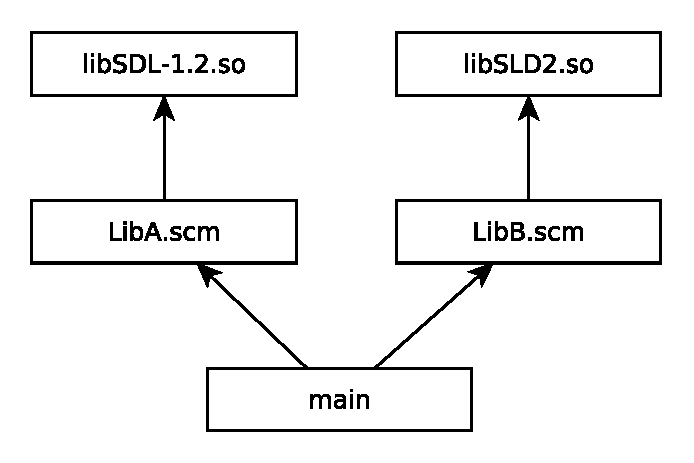
\includegraphics[width=4cm]{figures/SchemeLibrary}
%     \caption{Scheme}
%     \label{fig:1}
%   \end{center}
% \end{figure}
%%
%%Voici une insertion de plusieurs figures:
%%\begin{figure}[ht]
%%  \begin{center}
%%    \subfigure[Un cercle.]{\label{fig:2} 
\includegraphics[angle=-90,
%%      width=2.9cm]{figures/cercle}} \hspace{2cm}
%%    \subfigure[Un carré.]{\label{fig:3} 
\includegraphics[angle=-90,
%%      width=2.9cm]{figures/carre}}
%%    \caption{Des figures}
%%    \label{fig:4}
%%  \end{center}
%%\end{figure}

%%--------------%
%%     index    %
%%--------------%

%% S'il y a lieu, décommenter la ligne pour mettre votre index

%%\printindex

%%------------------------------------------------- %
%%         références --- bibliographie             %
%%------------------------------------------------- %

\nocite{*}
\bibliographystyle{plain-fr}
\bibliography{references.bib}

%\begin{thebibliography}{DDDD}
%
%\bibitem[A]{ams:guide}
%  {\scshape American Mathematical Society},
%  \emph{\AmS\LaTeX{} Version 1.1 User's Guide},
%  Amer. Math. Soc., Providence, R.~I., 1991.
%
%\bibitem[GMS]{latex2e:1}
%{\scshape M. Goossens, F. Mittelbach, and A. Samarin},
%\emph{The \LaTeX{} companion},
%Addison-Wesley, USA, 1994.
%
%\bibitem[H]{hahn:everyone}
%{\scshape J. Hahn},
%\emph{\LaTeX{} for Everyone: A reference guide and tutorial for
%    typesetting documents using a computer},
%     Personal \TeX, Inc., Mill Valley, CA., 1991.
%
%\bibitem[L]{lamport:latex}
%{\scshape Leslie Lamport},
%\emph{\LaTeX{} -- A Document Preparation System},
%     Addison-Wesley, Reading, Mass., 1986.
%
%\bibitem[M]{mckay:sty}
%{\scshape W. McKay},
%\emph{udemmem-l.sty}, fichier \LaTeX,  rédigé pour le compte de
%l'Université de Montréal, 1993.
%
%\bibitem[S]{spivak:joy}
%{\scshape M. D. Spivak},
%\emph{The Joy of \TeX{}}, second edition,
%     Amer. Math. Soc., Providence, R.~I., 1990.
%
%\bibitem[T]{latex2e:2}
%{\scshape \TeX{} User Group},
%\emph{\LaTeX2e for classand package writers},
%1995, disponible sur le web.
%
%\end{thebibliography}

%%------------------------------------------------- %
%%                  Annexe A                        %
%%------------------------------------------------- %

\appendix
\chapter{Information des environnement de test}
\label{ch:annexeA}

\begin{figure}[ht]
  \centering
\begin{mplisting}{1}
Architecture:          x86_64
CPU op-mode(s):        32-bit, 64-bit
CPU(s):                4
Thread(s) per core:    1
Core(s) per socket:    4
Vendor ID:             GenuineIntel
Model name:            Intel(R) Core(TM) i7-7700K CPU @ 4.20GHz
CPU MHz:               4200.000
CPU min MHz:           800.0000
Storage:               216GB (NVME)
RAM:                   16GB
Swap:                  16GB
C Compiler             gcc (Debian 6.3.0-18+deb9u1) 6.3.0 20170516
Ethernet Speed         1Gbps
\end{mplisting}
  \caption{La spécification de la machine arctic qui est utilisé comme nœud de destination dans
  l'ensemble des tests. Cette machine, nommé \MMM[x86/Linux] est refroidit au liquide.}
\end{figure}

\begin{figure}[ht]
  \begin{mplisting}{1}
Architecture:        armv7l
Byte Order:          Little Endian
CPU(s):              4
Thread(s) per core:  1
Core(s) per socket:  4
Vendor ID:           ARM
Model name:          Cortex-A72
CPU max MHz:         1500.0000
CPU min MHz:         600.0000
OS:                  Linux tictoc 4.19.66-v7l+ #1253 SMP
Hostname:            tictoc.iro.umontreal.ca
Storage:             26GB (sdcard)
RAM:                 2GB
Swap:                2GB
C Compiler           gcc (Raspbian 8.3.0-6+rpi1) 8.3.0
Ethernet Speed       1Gbps
\end{mplisting}
  \caption{La spécification du CPU du Raspberry Pi \MMM[ARM/Linux] utilisé dans
    les tests.}
\end{figure}

\begin{figure}[ht]
  \begin{mplisting}{1}
Architecture:        x86_64
CPU(s):              12
Thread(s) per core:  2
Core(s) per socket:  6
Model name:          Intel(R) Core(TM) i7-8700B CPU @ 3.20GHz
OS:                  Darwin Kernel Version 19.2.0
Hostname:            gambit.iro.umontreal.ca
Storage:             1TB (SSD)
RAM:                 32GB
Network Speed:       1Gbps
\end{mplisting}
  \caption{La spécification de la machine \MMM[x86/macOS] qui roule mac OS.}
\end{figure}

%
%\section{Section un de l'Annexe A}
%
%texte
%
%\chapter{Les différentes parties et leur ordre d'apparition}
%
%J'ajoute ici les différentes parties d'un mémoire ou d'une thèse ainsi
%que leur ordre d'apparition tel que décrit dans le guide de
%présentation des mémoires et des thèses de la Faculté des études
%supérieures.  Pour plus d'information, consultez le guide sur le site
%web de la facutlé (www.fesp.umontreal.ca).
%
%\begin{table}[htbp]
%  \begin{center}
%    \begin{tabular}{|lr|}\hline
%      1. les couvertures conformes & obligatoires\\
%      2. les pages de garde & obligatoires\\
%      3. la page de titre & obligatoire\\
%      4. l'identification du jury& obligatoire\\
%      5. le résumé en français et les mots clés français& obligatoires\\
%      6. le résumé en anglais et les mots clés anglais & obligatoires\\
%      8. le résumé de vulgarisation& facultatif\\
%      9. la table des matières, la liste des tableaux,\phantom{un fantome d'espace}&\\ \phantom{9. } la liste des figures & obligatoires\\
%      10. la liste des sigles, la liste des abréviations& obligatoires\\
%      11. la dédicace& facultative\\
%      12. les remerciements & facultatifs\\
%      13. l'avant-propos & facultatif\\
%      14. le corps de l'ouvrage& obligatoire\\
%      15. l'index analytique& facultatif\\
%      16. les sources documentaires & obligatoires\\
%      17. les appendices (annexes) & facultatifs\\
%      18. le curriculum vitæ & facultatif\\
%      19. les documents spéciaux & facultatifs\\\hline
%    \end{tabular}
%    \caption{Liste des parties}
%  \end{center}
%\end{table}

\end{document}
